\documentclass[11pt,a4paper]{article}

\usepackage[utf8]{inputenc}
\usepackage[T1]{fontenc}
\usepackage{lmodern}
\usepackage[brazilian]{babel}
\usepackage[margin=2.5cm]{geometry}
\usepackage{amsmath,amssymb}
\usepackage{graphicx}
\usepackage{caption}
\usepackage{subcaption}
\usepackage{float}
\usepackage{array}
\usepackage{tabularx}
\usepackage{xcolor}
\usepackage{indentfirst}
\usepackage{titlesec}
\usepackage{url}
% Opcional (descomentar no Overleaf ou se o pacote pdfescape estiver instalado no MiKTeX):
% \usepackage[colorlinks=true,linkcolor=blue!55!black,citecolor=blue!55!black,urlcolor=blue!55!black]{hyperref}

\captionsetup{font=small,labelfont=bf}
\graphicspath{{figuras/}}

% Macros auxiliares para tabelas com estilo academico limpo
\newcommand{\toprule}{\noalign{\hrule height 0.9pt}\noalign{\vskip 2pt}}
\newcommand{\midrule}{\noalign{\vskip 2pt}\noalign{\hrule height 0.45pt}\noalign{\vskip 2pt}}
\newcommand{\bottomrule}{\noalign{\vskip 2pt}\noalign{\hrule height 0.9pt}}
\renewcommand{\arraystretch}{1.18}

% Ajuste do titulo da bibliografia para o padrao solicitado em Portugues
\addto\captionsbrazilian{\renewcommand{\refname}{Refer\^{e}ncias Bibliogr\'{a}ficas}}

% Configuracao de espacamento discreto nos titulos de secao
\titleformat{\section}{\large\bfseries}{\thesection.}{0.6em}{}
\titleformat{\subsection}{\normalsize\bfseries}{\thesubsection}{0.6em}{}
\titleformat{\subsubsection}{\normalsize\itshape\bfseries}{\thesubsubsection}{0.6em}{}

\title{\textbf{Modelagem Comportamental 4D, Seguran\c{c}a de Hardware e Prototipagem Visual de Circuitos Polim\'{o}rficos Baseados em Transistores BP SB-FET em Ambiente Aberto}}

% TODO: Preencher autores, afiliacoes e e-mails na versao final
\author{
  Autor 1\thanks{Departamento / Institui\c{c}\~{a}o --- E-mail: \texttt{autor1@instituicao.edu.br}} \and
  Autor 2\thanks{Departamento / Institui\c{c}\~{a}o --- E-mail: \texttt{autor2@instituicao.edu.br}}
}

\date{\today}

\begin{document}

\maketitle

\begin{abstract}
\noindent\textit{[Resumo reservado para reda\c{c}\~{a}o final ap\'{o}s a conclus\~{a}o da Introdu\c{c}\~{a}o e do Referencial Te\'{o}rico. Este trabalho documenta a tradu\c{c}\~{a}o comportamental 4D do transistor ambipolar 2D de f\'{o}sforo negro (BP SB-FET) para \texttt{ngspice-47}, sua valida\c{c}\~{a}o cruzada frente ao HSPICE, a caracteriza\c{c}\~{a}o em ultra-baixa tens\~{a}o, primitivas polim\'{o}rficas, SRAM 6T com bloqueio de reten\c{c}\~{a}o, somador completo criptogr\'{a}fico, fronteiras sob tens\~{o}es n\~{a}o padronizadas, compromisso entre assimetria DPA e custo em sete tuplas polim\'{o}rficas e a plataforma web interativa BP-FET Studio.]}
\end{abstract}

\vspace{0.5em}
\noindent\textbf{Palavras-chave:} Transistores 2D; F\'{o}sforo Negro; L\'{o}gica Polim\'{o}rfica; Seguran\c{c}a de Hardware; An\'{a}lise Diferencial de Pot\^{e}ncia; SRAM 6T; \texttt{ngspice-47}.

\section{Introdu\c{c}\~{a}o}\label{sec:introducao}

\noindent\textit{[Se\c{c}\~{a}o reservada para reda\c{c}\~{a}o posterior.]}

% TODO: Inserir contextualizacao sobre seguranca de hardware em tecnologias CMOS
% convencionais versus dispositivos 2D reconfiguraveis, lacuna quanto ao uso
% de ferramentas proprietarias (HSPICE/Verilog-A e MATLAB), objetivos gerais e
% especificos deste trabalho e organizacao das secoes do artigo.

\section{Referencial Te\'{o}rico}\label{sec:referencial}

\noindent\textit{[Se\c{c}\~{a}o reservada para reda\c{c}\~{a}o posterior.]}

% TODO: Inserir fundamentacao teorica sobre:
% 1. Fisica de transistores bidimensionais de fosforo negro (BP SB-FET),
%    barreiras Schottky, tunelamento WKB e supressao ambipolar via porta de polaridade.
% 2. Arquitetura de cinco terminais (d, g, s, g1, g2) e portas logicas polimorficas.
% 3. Fundamentos de seguranca de hardware: logic locking, camuflagem,
%    ataques por canal lateral (DPA) e bloqueio de memoria SRAM (SNM e Read-Assist).

\section{Metodologia}\label{sec:metodologia}

\subsection{Fluxo Computacional Aberto e Organiza\c{c}\~{a}o da Su\'{i}te Experimental}\label{sec:met_fluxo}

Todo o desenvolvimento experimental e num\'{e}rico deste trabalho foi estruturado em um ambiente computacional integralmente aberto e reproduz\'{i}vel, eliminando a depend\^{e}ncia original de ferramentas comerciais propriet\'{a}rias---nomeadamente Synopsys HSPICE com suporte a Verilog-A (\texttt{\$table\_model}) e MATLAB---empregadas nos arquivos de refer\^{e}ncia de Wu et al.~\cite{wu2020reconfigurable}. O motor de simula\c{c}\~{a}o el\'{e}trica adotado \'{e} o \texttt{ngspice-47} (execut\'{a}vel em modo lote \texttt{ngspice\_con.exe}), acoplado a rotinas em Python (\texttt{numpy}, \texttt{pandas} e \texttt{matplotlib}) respons\'{a}veis pela gera\c{c}\~{a}o parametrizada de netlists SPICE, extra\c{c}\~{a}o automatizada de m\'{e}tricas, an\'{a}lises estat\'{i}sticas e produ\c{c}\~{a}o de figuras.

Para assegurar rastreabilidade e verifica\c{c}\~{a}o cont\'{i}nua, os experimentos foram organizados em oito m\'{o}dulos aut\^{o}nomos (\texttt{00} a \texttt{07}) sob o diret\'{o}rio \texttt{experimentos/}, executados sequencialmente pelo orquestrador \texttt{run\_all.py}, que re-simula todas as netlists e valida a integridade dos 66 artefatos gerados (bibliotecas, netlists, tabelas CSV e figuras). Complementarmente, construiu-se uma plataforma web interativa de prototipagem visual (\textit{BP-FET Studio}, em \texttt{simulador\_web/}) conectada diretamente ao \texttt{ngspice-47}. A Tabela~\ref{tab:resumo_modulos} sintetiza o escopo metodol\'{o}gico de cada componente da su\'{i}te.

\begin{table}[htbp]
\centering
\caption{Estrutura da su\'{i}te experimental em \texttt{ngspice-47} + Python e plataforma visual.}
\label{tab:resumo_modulos}
\footnotesize
\begin{tabularx}{\textwidth}{l l X l}
\toprule
\textbf{M\'{o}dulo} & \textbf{Dom\'{i}nio / An\'{a}lise} & \textbf{Escopo Metodol\'{o}gico} & \textbf{Principais Entregas} \\
\midrule
\texttt{00} & Dispositivo (DC) & Tradu\c{c}\~{a}o 4D das tabelas experimentais para SPICE nativo e valida\c{c}\~{a}o cruzada contra \texttt{.printtr0} do HSPICE. & \texttt{bp\_ari\_ngspice.lib}, 5 netlists, 2 CSVs, 4 figs. \\
\texttt{01} & Inversor 2T (DC/Tran) & Varreduras $V_{DD}$ de $1{,}0\ \text{V}$ a $0{,}2\ \text{V}$ com e sem compensa\c{c}\~{a}o de $V_{fb}$; comuta\c{c}\~{a}o transiente ($0{,}5\ \text{fF}$). & 2 netlists, 1 CSV, 2 figs. \\
\texttt{02} & Portas 4T (Tran) & Transmuta\c{c}\~{a}o din\^{a}mica em $t=20\ \text{ns}$ para \texttt{NAND}$\leftrightarrow$\texttt{NOR} ($0{,}8\ \text{V}$) e \texttt{XOR}$\leftrightarrow$\texttt{XNOR} ($1{,}5\ \text{V}$). & 2 netlists, 1 CSV, 2 figs. \\
\texttt{03} & DPA e Ru\'{i}do (DC/Estat.) & Portabilidade Python dos conjuntos DPA, Monte Carlo 3D ($N=250$) e reten\c{c}\~{a}o; varredura $5\times 5$ no \texttt{ngspice}. & 1 netlist, 3 CSVs, 4 figs. \\
\texttt{04} & SRAM 6T (Tran/DC) & Implementa\c{c}\~{a}o do Mecanismo B ($30\ \text{ns}$), curvas borboleta, SNM e \textit{Wordline Read-Assist} ($0{,}30\ \text{V}$). & 2 netlists, 1 CSV, 2 figs. \\
\texttt{05} & Full Adder 28T (Tran) & Somador polim\'{o}rfico multiest\'{a}gio com chave $(K_1, K_0)$, convers\~{a}o de n\'{i}vel e Dist\^{a}ncia de Hamming. & 1 netlist, 1 CSV, 2 figs. \\
\texttt{06} & Fronteiras (Tran escada) & Varredura de 292 pontos em tens\~{o}es n\~{a}o padronizadas dentro do dom\'{i}nio medido das LUTs. & 3 netlists, 2 CSVs, 3 figs. \\
\texttt{07} & Pareto DPA e FA (Tran) & Avalia\c{c}\~{a}o de 7 tuplas polim\'{o}rficas, Monte Carlo ($N=250$) e \textit{benchmark} de Full Adder em 3 perfis. & 4 netlists, 3 CSVs, 4 figs. \\
\texttt{Web} & Plataforma Interativa & Compilador de grafos alto/baixo n\'{i}vel para SPICE, Raio-X de transistores, oscilosc\'{o}pio DPA e testes. & Servidor HTTP, compilador, su\'{i}te E2E \\
\bottomrule
\end{tabularx}
\end{table}

\subsection{Tradu\c{c}\~{a}o do Modelo Comportamental 4D do BP SB-FET para \texttt{ngspice-47}}\label{sec:met_modelo}

No modelo original em Verilog-A (\texttt{bp\_ari.va}), o transistor ambipolar de f\'{o}sforo negro (\textit{Black Phosphorus Schottky-Barrier FET} --- BP SB-FET) \'{e} representado por um bloco \texttt{ari} de cinco terminais (\texttt{d, g, s, g1, g2}) parametrizado pela largura relativa $W$, o qual consulta duas tabelas experimentais quadridimensionais (\texttt{BP\_ARI\_\allowbreak dataN.txt}, com 1.810 linhas, e \texttt{BP\_ARI\_\allowbreak dataP.txt}, com 759 linhas) por meio da diretiva \texttt{\$table\_model}~\cite{wu2020reconfigurable}. Como o \texttt{ngspice-47} n\~{a}o executa diretamente tabelas 4D via \texttt{\$table\_model}, desenvolveu-se no M\'{o}dulo \texttt{00} (\texttt{gerar\_\allowbreak modelo\_\allowbreak e\_\allowbreak validar.py}) o subcircuito comportamental nativo \texttt{.subckt ARI d g s g1 g2 W=1.0} (\texttt{bp\_ari\_\allowbreak ngspice.lib}), em sua vers\~{a}o refinada \texttt{v2} (Superf\'{i}cie 4D).

Para suportar circuitos bidirecionais nos quais dreno e fonte trocam de papel conforme o vetor de entrada ou a chave de polaridade---como portas \textit{pass-transistor} \texttt{XOR}/\texttt{XNOR}, transistores de acesso da SRAM e seguidores de fonte no estado bloqueado---, o subcircuito define potenciais de refer\^{e}ncia bilaterais efetivos:
\begin{equation}\label{eq:bilateral_ref}
V_{g,n} = V_g - \min(V_d, V_s), \quad V_{g1,n} = V_{g1} - \min(V_d, V_s),
\end{equation}
\begin{equation}\label{eq:bilateral_ref_p}
V_{g,p} = V_g - \max(V_d, V_s), \quad V_{g1,p} = V_{g1} - \max(V_d, V_s).
\end{equation}
Essas express\~{o}es preservam exatamente as polariza\c{c}\~{o}es nominais quando $V_{ds} \ge 0$ no ramo \textit{n-FET} e $V_{ds} \le 0$ no ramo \textit{p-FET}, mantendo continuidade de corrente na invers\~{a}o de $V_{ds}$.

Sobre esse referencial, a superf\'{i}cie de transfer\^{e}ncia bidimensional $(V_{g1}, V_{g2})$ em $|V_{ds}| = 0{,}8\ \text{V}$ \'{e} reconstru\'{i}da por interpola\c{c}\~{a}o bilinear atrav\'{e}s de fun\c{c}\~{o}es-chap\'{e}u lineares por partes (\texttt{pwl}), com travamento plano externo (\textit{clamping}) em $\pm 1000\ \text{V}$ para evitar extrapola\c{c}\~{o}es n\~{a}o f\'{i}sicas e garantir converg\^{e}ncia no solucionador MNA:
\begin{itemize}
    \item \textbf{Ramo \textit{n-FET}:} $7 \times 4 = 28$ fatias experimentais cobrindo $V_{g1} \in [-0{,}1;\ 1{,}1]\ \text{V}$ (em passos de $0{,}2\ \text{V}$) e $V_{g2} \in \{0{,}2;\allowbreak\ 0{,}4;\allowbreak\ 0{,}8;\allowbreak\ 1{,}0\}\ \text{V}$, varridas em $V_{g,n} \in [-0{,}8;\ 1{,}1]\ \text{V}$.
    \item \textbf{Ramo \textit{p-FET}:} $8 \times 4 = 32$ fatias experimentais cobrindo $V_{g1} \in [-1{,}5;\ -0{,}1]\ \text{V}$ (em passos de $0{,}2\ \text{V}$) e $V_{g2} \in \{-1{,}5;\allowbreak\ -1{,}2;\allowbreak\ -1{,}1;\allowbreak\ -0{,}9\}\ \text{V}$, varridas em $V_{g,p} \in [-1{,}5;\ 0{,}0]\ \text{V}$. A inclus\~{a}o expl\'{i}cita do plano medido em $V_{g2} = -1{,}5\ \text{V}$ captura o deslocamento real de tens\~{a}o de banda plana ($\Delta V_{fb} \approx -0{,}25\ \text{V}$) presente nos dados experimentais, o qual n\~{a}o era reproduzido pela aproxima\c{c}\~{a}o escalar preliminar (\texttt{v1}).
\end{itemize}

Para modelar as regi\~{o}es de tr\'{i}odo e satura\c{c}\~{a}o em fun\c{c}\~{a}o simult\^{a}nea da porta principal e da tens\~{a}o dreno-fonte, a vers\~{a}o \texttt{v2} substitui o fator anal\'{i}tico global $\tanh(2{,}5\,V_{ds})/\tanh(2{,}0)$ da vers\~{a}o \texttt{v1} por fatores bidimensionais $f_{ds,n}(V_{g,n}, V_{ds})$ (6 fatias em $V_{g,n} \in [0{,}1;\ 1{,}1]\ \text{V}$) e $f_{ds,p}(V_{g,p}, V_{ds})$ (5 fatias em $V_{g,p} \in [-1{,}5;\ -0{,}7]\ \text{V}$), extra\'{i}dos das varreduras experimentais de sa\'{i}da, normalizados em $|V_{ds}| = 0{,}8\ \text{V}$ e estendidos como fun\c{c}\~{o}es \texttt{pwl} \'{i}mpares estritamente monot\^{o}nicas com condut\^{a}ncia \^{o}hmica finita em $V_{ds} = 0\ \text{V}$. A corrente de dreno-fonte \'{e} ent\~{a}o imposta pela fonte comportamental:
\begin{equation}\label{eq:bp_current}
I_{ds} = W \cdot \begin{cases}
I_n(V_{g1,n},\, V_{g2,s},\, V_{g,n}) \cdot f_{ds,n}(V_{g,n},\, V_{ds}), & \text{se } V(g2,s) > 0\ \text{V}, \\
I_p(V_{g1,p},\, V_{g2,s},\, V_{g,p}) \cdot f_{ds,p}(V_{g,p},\, V_{ds}), & \text{se } V(g2,s) \le 0\ \text{V},
\end{cases}
\end{equation}
acoplada em paralelo a um resistor $R_{\mathrm{gmin}} = 10^{12}\ \Omega$ para estabilidade num\'{e}rica. Importa registrar que, assim como o arquivo \texttt{bp\_ari.va} original, a biblioteca \texttt{bp\_ari\_ngspice.lib} \'{e} puramente quase-est\'{a}tica e n\~{a}o inclui capacit\^{a}ncias intr\'{i}nsecas de porta ou sobreposi\c{c}\~{a}o ($C_{gs}, C_{gd}, C_{g2s}$); por esse motivo, todas as simula\c{c}\~{o}es transientes descritas a seguir inserem capacit\^{a}ncias nodais e de carga expl\'{i}citas ($0{,}05\ \text{fF}$ a $1{,}0\ \text{fF}$).

A valida\c{c}\~{a}o do modelo foi realizada por meio de cinco netlists DC (\texttt{sim\_N\_transfer.sp}, \texttt{sim\_P\_transfer.sp}, \texttt{sim\_N\_output.sp}, \texttt{sim\_P\_output.sp} e \texttt{sim\_polarity\_gate.sp}), comparando as vers\~{o}es \texttt{v1} e \texttt{v2} diretamente com os registros oficiais \texttt{.printtr0} gerados pelo Synopsys HSPICE por meio da raiz do erro quadr\'{a}tico m\'{e}dio (RMSE), erro absoluto m\'{e}dio (MAE), erro m\'{a}ximo e coeficiente de determina\c{c}\~{a}o ($R^2$). Extra\'{i}ram-se tamb\'{e}m $I_{\mathrm{on}}$, $I_{\mathrm{off}}$, raz\~{a}o $I_{\mathrm{on}}/I_{\mathrm{off}}$ e inclina\c{c}\~{a}o m\'{i}nima de sublimiar ($SS_{\min}$) em $|V_{ds}| = 0{,}8\ \text{V}$.

\subsection{Caracteriza\c{c}\~{a}o do Inversor em Ultra-Baixa Tens\~{a}o e Portas Polim\'{o}rficas}\label{sec:met_inv_poly}

No M\'{o}dulo \texttt{01}, o inversor l\'{o}gico complementar ($W_{\mathrm{PU}} = W_{\mathrm{PD}} = 1{,}0$) foi configurado com polariza\c{c}\~{a}o nominal de banda de condu\c{c}\~{a}o (\textit{pull-down} \textit{n-FET} com $V_{g1,n} = 1{,}1\ \text{V},\ V_{g2,n} = 0{,}8\ \text{V}$ e \textit{pull-up} \textit{p-FET} com $V_{g1,p} = V_{DD} - 1{,}5\ \text{V},\ V_{g2,p} = V_{DD} - 1{,}2\ \text{V}$). Executaram-se varreduras DC em \texttt{inv\_vtc.sp} ($0 \to V_{DD}$ em passos de $2\ \text{mV}$) para $V_{DD} \in \{1{,}0;\ 0{,}8;\ 0{,}6;\ 0{,}4;\ 0{,}2\}\ \text{V}$ sob duas configura\c{c}\~{o}es:
\begin{enumerate}
    \item \textbf{Acoplamento direto:} entrada $V_{\mathrm{in}}$ aplicada sem deslocamento aos terminais de porta (\texttt{off}$_n = \text{off}_p = 0$).
    \item \textbf{Compensa\c{c}\~{a}o eletrost\'{a}tica de $V_{fb}$:} inser\c{c}\~{a}o de deslocamentos controlados $\text{off}_n = -0{,}02 - 0{,}5\,V_{DD}$ e $\text{off}_p = 0{,}5\,V_{DD} - 0{,}58$, de modo que em $V_{\mathrm{in}} = V_{DD}/2$ ambos os ramos operem alinhados no ponto de maior ganho de sublimiar ($V_{gs,n,\mathrm{eff}} = -0{,}02\ \text{V}$ e $V_{gs,p,\mathrm{eff}} = -0{,}58\ \text{V}$).
\end{enumerate}
A partir das curvas VTC extra\'{i}ram-se a excurs\~{a}o percentual $(V_{\mathrm{out}}(0)-V_{\mathrm{out}}(V_{DD}))/V_{DD}$, a tens\~{a}o de invers\~{a}o $V_M$, o ganho diferencial m\'{a}ximo $|A_v|_{\max} = \max|dV_{\mathrm{out}}/dV_{\mathrm{in}}|$ e as margens de ru\'{i}do est\'{a}ticas $NM_L$ e $NM_H$ pelos pontos de tang\^{e}ncia unit\'{a}ria ($dV_{\mathrm{out}}/dV_{\mathrm{in}} = -1$). Adicionalmente, \texttt{inv\_tran.sp} avaliou a resposta transiente ($14\ \text{ns}$) sob carga capacitiva $C_{\mathrm{load}} = 0{,}5\ \text{fF}$ para $V_{DD} = 1{,}0\ \text{V}$ e $0{,}6\ \text{V}$.

No M\'{o}dulo \texttt{02}, simularam-se em regime transiente ($40\ \text{ns}$, passo de $20\ \text{ps}$, carga $C_{\mathrm{out}} = 0{,}3\ \text{fF}$) as duas primitivas polim\'{o}rficas de 4 transistores propostas em~\cite{wu2020reconfigurable}, percorrendo exaustivamente os vetores $(A,B) \in \{00, 01, 10, 11\}$ em janelas de $5\ \text{ns}$ com comuta\c{c}\~{a}o da chave $\text{Key}$ em $t = 20\ \text{ns}$:
\begin{itemize}
    \item \textbf{\texttt{NAND} $\leftrightarrow$ \texttt{NOR} (\texttt{poly\_nand\_nor.sp}, $V_{DD} = 0{,}8\ \text{V}$):} rede superior paralela ($W=1{,}0$) conectada a \texttt{rtop}/\texttt{gtop} e rede inferior em s\'{e}rie ($W=2{,}0$, capacit\^{a}ncia no n\'{o} intermedi\'{a}rio $C_{n1}=0{,}1\ \text{fF}$) conectada a \texttt{rbot}/\texttt{gbot}. Em $\text{Key}=0$ (\texttt{NAND}), aplica-se $(r_{\mathrm{top}}, g_{\mathrm{top}}, r_{\mathrm{bot}}, g_{\mathrm{bot}}) = (0{,}8;\ -0{,}4;\ 0{,}0;\ 0{,}8)\ \text{V}$; em $\text{Key}=1$ (\texttt{NOR}), permutam-se trilhos e polaridades para $(0{,}0;\ 0{,}8;\ 0{,}8;\ -0{,}7)\ \text{V}$.
    \item \textbf{\texttt{XOR} $\leftrightarrow$ \texttt{XNOR} (\texttt{poly\_xor\_xnor.sp}, $V_{DD} = 1{,}5\ \text{V}$, $V_{\mathrm{in}} = 1{,}1\ \text{V}$):} quatro transistores id\^{e}nticos ($W=1{,}0$) em ponte sim\'{e}trica acionados por entradas diferenciais $(A,\overline{A})$ nos terminais \texttt{g} e $(B,\overline{B})$ nos terminais auxiliares \texttt{g1}, alternando $(r_{\mathrm{top}}, g_{\mathrm{top}}, r_{\mathrm{bot}}, g_{\mathrm{bot}})$ entre $(1{,}5;\ 0{,}0;\ 0{,}0;\ 0{,}8)\ \text{V}$ ($\text{Key}=0$, \texttt{XOR}) e $(0{,}0;\ 0{,}8;\ 1{,}5;\ 0{,}0)\ \text{V}$ ($\text{Key}=1$, \texttt{XNOR}).
\end{itemize}

\subsection{Seguran\c{c}a contra DPA, Robustez Estat\'{i}stica e Fronteiras de Tens\~{a}o}\label{sec:met_dpa_fronteira}

No M\'{o}dulo \texttt{03}, substitu\'{i}ram-se integralmente os \textit{scripts} MATLAB de~\cite{wu2020reconfigurable} por rotinas Python em \texttt{analisar\_dpa\_e\_robustez.py} para processar as formas de onda transientes de corrente $|I(V_{DD})|$ das fam\'{i}lias \texttt{NAND}/\texttt{NOR} e \texttt{XOR}/\texttt{XNOR} (janela de $0$ a $30\ \mu\text{s}$), os conjuntos Monte Carlo de 250 amostras de flutua\c{c}\~{a}o simult\^{a}nea nos trilhos $V_{DD}$ e $V_{SS}$ por porta (classificando os n\'{i}veis l\'{o}gicos em torno do limiar $0{,}40\ \text{V}$) e as s\'{e}ries temporais de reten\c{c}\~{a}o do n\'{o} flutuante \texttt{bblc1} at\'{e} $111\ \mu\text{s}$ ap\'{o}s pulsos de $100\ \text{ns}$, $250\ \text{ns}$ e $500\ \text{ns}$. Como valida\c{c}\~{a}o param\'{e}trica independente sobre o modelo traduzido, executou-se no \texttt{ngspice-47} a netlist \texttt{sim\_supply\_noise.sp} com uma grade $5 \times 5$ variando $V_{DD} \in [0{,}65;\ 0{,}95]\ \text{V}$ e $V_{SS} \in [-0{,}10;\ +0{,}10]\ \text{V}$ na porta \texttt{NAND} 4T, mensurando a margem diferencial est\'{a}tica $V_{\mathrm{out}}(00) - V_{\mathrm{out}}(11)$.

No M\'{o}dulo \texttt{06}, investigou-se o comportamento das portas polim\'{o}rficas sob tens\~{o}es n\~{a}o padronizadas por meio de varreduras PWL em escada com quatro c\'{e}lulas paralelas correspondentes aos vetores \texttt{00}, \texttt{01}, \texttt{10} e \texttt{11}. Com rigor metodol\'{o}gico, todas as polariza\c{c}\~{o}es foram mantidas estritamente no interior do dom\'{i}nio experimentalmente medido nas tabelas LUT: $V(g2,s)_n \in [+0{,}20;\ +1{,}00]\ \text{V}$ e $V(g2,s)_p \in [-1{,}50;\ -0{,}90]\ \text{V}$, evitando a faixa n\~{a}o medida $(-0{,}90;\ +0{,}20)\ \text{V}$. Ao todo, simularam-se 292 condi\c{c}\~{o}es operacionais distribu\'{i}das em tr\^{e}s experimentos:
\begin{enumerate}
    \item \textbf{\texttt{NAND}/\texttt{NOR} ($V_{DD} \times$ Polaridade, 70 pontos):} 7 n\'{i}veis de $V_{DD} \in \{0{,}25;\allowbreak\ 0{,}35;\allowbreak\ 0{,}50;\allowbreak\ 0{,}65;\allowbreak\ 0{,}80;\allowbreak\ 0{,}95;\allowbreak\ 1{,}10\}\ \text{V}$ combinados com 5 pares de polaridade na LUT ($\text{Sub-pol Min}\ +0{,}2/-0{,}9\ \text{V}$, $\text{Sub-pol Mod}\ +0{,}4/-1{,}1\ \text{V}$, $\text{Nom.\ NAND}\ +0{,}8/-1{,}2\ \text{V}$, $\text{Nom.\ NOR}\ +0{,}8/-1{,}5\ \text{V}$ e $\text{Sobre-pol}\ +1{,}0/-1{,}5\ \text{V}$) para $\text{Key} \in \{0, 1\}$.
    \item \textbf{\texttt{NAND}/\texttt{NOR} (Assimetria $V(g2,s)_n \times V(g2,s)_p$, 72 pontos):} grade $6 \times 6$ em $V_{DD} = 0{,}80\ \text{V}$ variando $V(g2,s)_n \in \{0{,}20;\allowbreak\ 0{,}30;\allowbreak\ 0{,}40;\allowbreak\ 0{,}60;\allowbreak\ 0{,}80;\allowbreak\ 1{,}00\}\ \text{V}$ e $V(g2,s)_p \in \{-0{,}90;\allowbreak\ -1{,}00;\allowbreak\ -1{,}10;\allowbreak\ -1{,}20;\allowbreak\ -1{,}35;\allowbreak\ -1{,}50\}\ \text{V}$ para $\text{Key} \in \{0, 1\}$.
    \item \textbf{\texttt{XOR}/\texttt{XNOR} ($V_{DD} \times V_{\mathrm{in}}$ e porta fixa, 150 pontos):} 5 n\'{i}veis de $V_{DD} \in \{0{,}60;\allowbreak\ 0{,}80;\allowbreak\ 1{,}00;\allowbreak\ 1{,}20;\allowbreak\ 1{,}50\}\ \text{V}$ $\times$ 5 amplitudes de entrada $V_{\mathrm{in}} \in \{0{,}40;\allowbreak\ 0{,}60;\allowbreak\ 0{,}80;\allowbreak\ 1{,}10;\allowbreak\ 1{,}30\}\ \text{V}$ sob polaridade nominal ($+0{,}8/-1{,}5\ \text{V}$) e sub-polarizada ($+0{,}2/-0{,}9\ \text{V}$) para ambas as chaves (100 pontos), mais 50 pontos avaliando $V_{g,\mathrm{top}} = 0\ \text{V}$ fixo em $V_{DD} \in [0{,}90;\ 1{,}50]\ \text{V}$.
\end{enumerate}
Cada vetor de sa\'{i}da normalizado $V_{\mathrm{out}}/V_{DD}$ foi discretizado em \texttt{'1'} ($\ge 0{,}75$), \texttt{'0'} ($\le 0{,}25$) ou \texttt{'X'} ($0{,}25 < V_{\mathrm{out}}/V_{DD} < 0{,}75$), classificando o ponto em \texttt{CORRETA}, \texttt{OUTRA\_FUNCAO} (n\'{i}veis digitais v\'{a}lidos realizando outra tabela booleana) ou \texttt{INDEFINIDO\_ANALOGICO} (presen\c{c}a de ao menos um estado \texttt{'X'}).

\subsection{C\'{e}lula SRAM 6T com Bloqueio de Reten\c{c}\~{a}o por Polaridade (Mecanismo B)}\label{sec:met_sram}

No M\'{o}dulo \texttt{04}, implementou-se em \texttt{ngspice-47} (\texttt{ARI\_sram\_mecB\_ngspice.sp}) uma c\'{e}lula de mem\'{o}ria SRAM 6T dotada de bloqueio de reten\c{c}\~{a}o por invers\~{a}o de polaridade (\textit{Mecanismo B}). Ao contr\'{a}rio das portas l\'{o}gicas polim\'{o}rficas que permutam os trilhos de energia, o Mecanismo B mant\'{e}m os barramentos de alimenta\c{c}\~{a}o estritamente fixos em $V_{DD} = 1{,}0\ \text{V}$ e $V_{SS} = 0{,}0\ \text{V}$, utilizando a chave criptogr\'{a}fica para inverter dinamicamente o tipo de condu\c{c}\~{a}o dos transistores dos dois inversores acoplados de forma cruzada.

Os seis transistores \texttt{ARI} seguem raz\~{o}es de largura dimensionadas para conciliar estabilidade de leitura e capacidade de escrita: \textit{pull-up} \texttt{XPU1}, \texttt{XPU2} com $W = 1{,}0$; \textit{pull-down} \texttt{XPD1}, \texttt{XPD2} com $W = 2{,}0$; e portas de acesso (\textit{pass-gates}) \texttt{XPG1}, \texttt{XPG2} com $W = 1{,}5$, com capacit\^{a}ncias nodais $C_q = C_{qb} = 1{,}0\ \text{fF}$. A Tabela~\ref{tab:sram_polarizacoes} especifica o esquema exato de polariza\c{c}\~{a}o adotado nos dois estados da chave. Em $\text{Key} = 0$ (modo autorizado), o ajuste de $V_{g2,\mathrm{PU}}$ foi sintonizado para $-0{,}2\ \text{V}$ ($V_{g2,s} = -1{,}2\ \text{V}$), evitando o deslocamento de banda plana de $V_{g2,s} = -1{,}5\ \text{V}$ identificado pelo modelo \texttt{v2}. Em $\text{Key} = 1$ (modo bloqueado), \texttt{XPU1}/\texttt{XPU2} assumem polaridade \textit{n-FET} e \texttt{XPD1}/\texttt{XPD2} assumem polaridade \textit{p-FET}, convertendo os inversores regenerativos em seguidores de fonte degradados e destruindo a biestabilidade.

\begin{table}[htbp]
\centering
\caption{Esquema de polariza\c{c}\~{a}o do Mecanismo B na c\'{e}lula SRAM 6T ($V_{DD}=1{,}0\ \text{V}$, $V_{SS}=0{,}0\ \text{V}$).}
\label{tab:sram_polarizacoes}
\footnotesize
\begin{tabularx}{\textwidth}{>{\raggedright\arraybackslash}p{2.3cm} >{\raggedright\arraybackslash}p{3.1cm} >{\raggedright\arraybackslash}p{2.9cm} >{\raggedright\arraybackslash}p{2.9cm} >{\raggedright\arraybackslash}X}
\toprule
\textbf{Estado da Chave} & \textbf{Pull-Up ($W=1{,}0$)} & \textbf{Pull-Down ($W=2{,}0$)} & \textbf{Pass-Gates ($W=1{,}5$)} & \textbf{Regime F\'{i}sico Resultante} \\
\midrule
$\text{Key}=0$ (Autorizado) & \textit{p-FET}: $V_{g1}=-0{,}5\ \text{V}$, $V_{g2}=-0{,}2\ \text{V}$ ($V_{g2,s}=-1{,}2\ \text{V}$) & \textit{n-FET}: $V_{g1}=+0{,}8\ \text{V}$, $V_{g2}=+1{,}1\ \text{V}$ & \textit{n-FET}: $V_{g1}=+1{,}8\ \text{V}$, $V_{g2}=+2{,}1\ \text{V}$ & Inversores CMOS complementares biest\'{a}veis \\
$\text{Key}=1$ (Bloqueado) & \textit{n-FET}: $V_{g1}=+1{,}8\ \text{V}$, $V_{g2}=+2{,}1\ \text{V}$ ($V_{g2,s}=+1{,}1\ \text{V}$) & \textit{p-FET}: $V_{g1}=-1{,}5\ \text{V}$, $V_{g2}=-1{,}5\ \text{V}$ & \textit{n-FET}: $V_{g1}=+1{,}8\ \text{V}$, $V_{g2}=+2{,}1\ \text{V}$ & Seguidores de fonte cruzados (colapso monost\'{a}vel) \\
\bottomrule
\end{tabularx}
\end{table}

O protocolo transiente de $30\ \text{ns}$ compreende quatro fases: (1)~escrita do bit \texttt{'1'} em $0\text{--}6\ \text{ns}$ sob $\text{Key}=0$ ($\mathrm{WL}=1{,}0\ \text{V}$ entre $2$ e $6\ \text{ns}$, $\mathrm{BL}=1{,}0\ \text{V}$, $\mathrm{BLB}=0{,}0\ \text{V}$); (2)~reten\c{c}\~{a}o ativa em $6\text{--}15\ \text{ns}$ ($\mathrm{WL}=0\ \text{V}$, crit\'{e}rio $\Delta V_{\mathrm{Key0}} = |V(q)-V(qb)| > 0{,}80\ \text{V}$ em $t=12\ \text{ns}$); (3)~ativa\c{c}\~{a}o do bloqueio em $t=15\ \text{ns}$ ($\text{Key}=1$, colapso verificado em $t=18\ \text{ns}$ com crit\'{e}rio $\Delta V_{\mathrm{Collapse1}} < 0{,}15\ \text{V}$); e (4)~tentativa de reescrita do bit oposto entre $20$ e $24\ \text{ns}$ sob $\text{Key}=1$, seguida de novo fechamento de $\mathrm{WL}$ e verifica\c{c}\~{a}o de falha de reten\c{c}\~{a}o em $t=28\ \text{ns}$ ($\Delta V_{\mathrm{Key1}} < 0{,}15\ \text{V}$).

Adicionalmente, \texttt{sram\_butterfly\_snm.sp} executa varreduras DC de meia-c\'{e}lula ($V_{\mathrm{in}} \in [0;\ 1{,}0]\ \text{V}$, passo de $5\ \text{mV}$) com \texttt{alterparam} para seis regimes combinando $\text{Key} \in \{0, 1\}$ e $\mathrm{WL} \in \{0{,}0\ \text{V}\ (\text{Hold}),\ 0{,}30\ \text{V}\ (\text{Wordline Underdrive Read-Assist}),\ 1{,}0\ \text{V}\ (\text{Read s/ Assist})\}$, com $\mathrm{BL}=1{,}0\ \text{V}$. A Margem de Ru\'{i}do Est\'{a}tica (SNM) \'{e} calculada geometricamente pelo maior quadrado inscrito no lobo da curva borboleta no referencial rotacionado de $45^\circ$:
\begin{equation}\label{eq:snm_45}
u = \frac{V_{qb} - V_q}{\sqrt{2}}, \quad v = \frac{V_{qb} + V_q}{\sqrt{2}}, \quad \mathrm{SNM} = \max_{u < 0} \frac{v_1(u) - v_2(u)}{\sqrt{2}},
\end{equation}
sobre uma grade uniforme de 2.000 pontos.

\subsection{Circuitos Combinacionais Criptogr\'{a}ficos e Mapeamento de Tuplas Polim\'{o}rficas}\label{sec:met_comb_tuplas}

No M\'{o}dulo \texttt{05}, demonstrou-se a escalabilidade multiest\'{a}gio em um Somador Completo de 1 bit (\textit{Full Adder} --- FA) de 28 transistores (\texttt{full\_adder\_polimorfico.sp}) controlado por chave de 2 bits $(K_1, K_0)$: (i)~est\'{a}gio \texttt{XXOR1} (4T em $1{,}5\ \text{V}$) controlado por $K_0$, produzindo $P = A \oplus B$ ($K_0=0$) ou $P = A \odot B$ ($K_0=1$); (ii)~bloco de condicionamento e convers\~{a}o de n\'{i}vel com quatro inversores (\texttt{2}$\times$ \texttt{BP\_INV08} a $0{,}8\ \text{V}$ e \texttt{2}$\times$ \texttt{BP\_INV11} a $1{,}1\ \text{V}$, totalizando 8T com deslocamento interno de $-0{,}27\ \text{V}$ na porta) para regenerar $(P, \overline{P})$ em ambos os dom\'{i}nios de tens\~{a}o; (iii)~est\'{a}gio \texttt{XXOR2} (4T em $1{,}5\ \text{V}$) gerando $\mathrm{Sum} = P \oplus C_{\mathrm{in}}$; e (iv)~\'{a}rvore de transporte \texttt{Cout} composta por tr\^{e}s portas polim\'{o}rficas \texttt{XG1}--\texttt{XG3} (12T em $0{,}8\ \text{V}$) controladas por $K_1$ (\texttt{NAND} em $K_1=0$ e \texttt{NOR} em $K_1=1$). Todas as quatro chaves $K_1 K_0 \in \{00, 01, 10, 11\}$ foram simuladas em $40\ \text{ns}$ sobre os 8 mintermos ($000 \to 111$, $5\ \text{ns}$ por vetor), com amostragem estabilizada em $[5i+3{,}5;\ 5i+4{,}8]\ \text{ns}$ e binariza\c{c}\~{a}o nos limiares de $0{,}75\ \text{V}$ (\texttt{Sum}) e $0{,}40\ \text{V}$ (\texttt{Cout}) para extra\c{c}\~{a}o da Dist\^{a}ncia de Hamming (HD).

No M\'{o}dulo \texttt{07}, conduziu-se um mapeamento sistem\'{a}tico do compromisso entre assimetria de corrente DPA, custo em \'{a}rea, desempenho din\^{a}mico, consumo energ\'{e}tico e robustez estat\'{i}stica em sete tuplas polim\'{o}rficas sob carga padronizada $C_{\mathrm{load}} = 0{,}3\ \text{fF}$:
\begin{itemize}
    \item \textbf{Cinco tuplas de 2 entradas (\texttt{tuplas\_\allowbreak 2entradas.sp}, ciclo de $25\ \text{ns}$ na sequ\^{e}ncia \texttt{00} $\to$ \texttt{01} $\to$ \texttt{10} $\to$ \texttt{11} $\to$ \texttt{00}):} \texttt{(NAND, NOR)} (4T, $V_{DD}=0{,}8\ \text{V}$), \texttt{(XOR, XNOR)} (4T n\'{u}cleo / 8T total com inversores de entrada, $1{,}5\ \text{V}$/$1{,}1\ \text{V}$), \texttt{(AND, OR)} (6T = est\'{a}gio \texttt{NAND/NOR} 4T seguido por inversor isolador \texttt{BP\_INV08} 2T, $0{,}8\ \text{V}$), \texttt{(NAND, XNOR)} e \texttt{(NOR, XOR)} (tuplas mistas de 6T n\'{u}cleo / 10T total em $1{,}5\ \text{V}$/$1{,}1\ \text{V}$ combinando rede \textit{pass-transistor} e ramos habilitados por chave).
    \item \textbf{Duas tuplas de 3 entradas (\texttt{tuplas\_\allowbreak 3entradas.sp}, ciclo de $45\ \text{ns}$ de \texttt{000} a \texttt{111} $\to$ \texttt{000}):} \texttt{(AOI21, OAI21)} (6T em topologia composta s\'{e}rie-paralela complementar, $0{,}8\ \text{V}$) e \texttt{(MAJ3, XOR3)} (n\'{u}cleo polim\'{o}rfico quad-sim\'{e}trico de 10T com multiplexa\c{c}\~{a}o local da fun\c{c}\~{a}o de maioria vs.\ paridade em $1{,}5\ \text{V}$, totalizando 18T ao incluir o est\'{a}gio gerador e condicionador $P = A \oplus B$).
\end{itemize}

A assimetria DPA relativa entre os dois modos de cada tupla foi padronizada conforme:
\begin{equation}\label{eq:dpa_asym}
\mathrm{DPA}_{\mathrm{asym}} = \frac{|I_{\mathrm{Modo\ 0}} - I_{\mathrm{Modo\ 1}}|}{\min(I_{\mathrm{Modo\ 0}},\, I_{\mathrm{Modo\ 1}})} \times 100\%,
\end{equation}
aplicada tanto aos picos de corrente de alimenta\c{c}\~{a}o quanto \`{a}s correntes m\'{e}dias e janelas espec\'{i}ficas de transi\c{c}\~{a}o ($0\to 1$ e $1\to 0$). Extra\'{i}ram-se igualmente a soma das larguras $\sum W$, os atrasos de propaga\c{c}\~{a}o m\'{e}dios $t_p = (t_{pLH} + t_{pHL})/2$ a $50\%$ da excurs\~{a}o, a pot\^{e}ncia m\'{e}dia $P_{\mathrm{m\acute{e}d}}$ e est\'{a}tica $P_{\mathrm{est}}$, a energia por chaveamento $E_{\mathrm{sw}}$ e o produto pot\^{e}ncia-atraso ($\mathrm{PDP} = P_{\mathrm{m\acute{e}d}} \cdot t_p$). Para avalia\c{c}\~{a}o estat\'{i}stica, \texttt{sim\_robustez\_tuplas.sp} simulou uma grade $3 \times 3$ no \texttt{ngspice-47} ($\Delta V_{DD} \in \{-10\%, 0\%, +10\%\}$ e $\Delta V_{SS} \in \{-50, 0, +50\}\ \text{mV}$), a partir da qual foram avaliadas $N = 250$ amostras Monte Carlo gaussianas ($\sigma_{V_{DD}} = 3{,}5\%$, $\sigma_{V_{SS}} = 18\ \text{mV}$).

Por fim, avaliou-se o impacto arquitetural dessas tuplas em um \textit{benchmark} de Full Adder 1-bit (\texttt{full\_adder\_perfis\_dpa.sp}, $40\ \text{ns}$, $C_{\mathrm{load}} = 0{,}3\ \text{fF}$) comparando tr\^{e}s perfis: \textbf{Perfil 1 (Baseline Comum)}, com 20T de n\'{u}cleo (\texttt{2}$\times$ \texttt{XOR} 4T + \texttt{4}$\times$ \texttt{INV} 2T + \texttt{MAJ3} 4T fixo, sem travamento l\'{o}gico); \textbf{Perfil 2 (Custo/Desempenho)}, com 28T substituindo o \textit{carry} por 3 portas \texttt{(NAND, NOR)} de 4T; e \textbf{Perfil 3 (Baixa Assimetria DPA)}, com 26T substituindo a \'{a}rvore \texttt{NAND}/\texttt{NOR} por uma \'{u}nica c\'{e}lula polim\'{o}rfica \texttt{(MAJ3, XOR3)} de 10T.

\subsection{Plataforma Interativa de Prototipagem e Simula\c{c}\~{a}o Visual (\textit{BP-FET Studio})}\label{sec:met_web}

Para democratizar a explora\c{c}\~{a}o dos circuitos reconfigur\'{a}veis sem exigir escrita manual de netlists, desenvolveu-se o ambiente web \textit{BP-FET Studio} (\texttt{simulador\_web/}), composto por um servidor HTTP/REST local em Python (\texttt{server.py} baseado em \texttt{ThreadingHTTPServer}, expondo as rotas \texttt{/api/health}, \texttt{/api/tuples}, \texttt{/api/templates} e \texttt{/api/simulate}), um compilador de grafos para SPICE (\texttt{spice\_compiler.py}), um cat\'{a}logo de oito circuitos-modelo (\texttt{templates\_catalog.py}) e uma interface gr\'{a}fica SVG/Canvas em HTML5/JavaScript.

O compilador opera em dois n\'{i}veis de abstra\c{c}\~{a}o sobre a biblioteca \texttt{bp\_ari\_ngspice.lib}:
\begin{itemize}
    \item \textbf{Alto N\'{i}vel (Portas Polim\'{o}rficas):} o usu\'{a}rio conecta blocos configur\'{a}veis entre as sete tuplas mapeadas e o inversor \texttt{INV}. O compilador insere automaticamente os est\'{a}gios de gera\c{c}\~{a}o diferencial $(A, \overline{A})$ e os inversores de convers\~{a}o de n\'{i}vel (\texttt{BP\_INV08} e \texttt{BP\_INV11}) sempre que blocos de $0{,}8\ \text{V}$ e $1{,}5\ \text{V}$ s\~{a}o encadeados em cascata mista.
    \item \textbf{Baixo N\'{i}vel (Transistores \texttt{ARI}):} permite a montagem direta de esquem\'{a}ticos el\'{e}tricos com inst\^{a}ncias de cinco terminais \texttt{(d, g, s, g1, g2)}, fontes DC e PWL dependentes ou n\~{a}o da chave $\text{Key}$, capacitores e pontas de prova.
\end{itemize}
Ao executar a simula\c{c}\~{a}o comparativa ($\text{Key}=0$ e $\text{Key}=1$), o sistema devolve \`{a} interface as s\'{e}ries reamostradas de tens\~{a}o nodal (animadas passo a passo sobre o esquem\'{a}tico), a assinatura de corrente $|I_{V_{DD}}(t)|$ para an\'{a}lise DPA, a tabela-verdade binarizada e o estado interno de cada transistor no modal \textit{Raio-X} (classificando a polaridade ativa em \textit{n-FET} ou \textit{p-FET} pelo crit\'{e}rio $V(g2, s) > 0\ \text{V}$ e o grau normalizado de condu\c{c}\~{a}o). Toda a cadeia \'{e} verificada pela su\'{i}te automatizada \texttt{test\_simulator.py}.

\section{Resultados}\label{sec:resultados}

\subsection{Valida\c{c}\~{a}o do Modelo BP SB-FET e Caracteriza\c{c}\~{a}o do Dispositivo}\label{sec:res_modelo}

A biblioteca comportamental nativa \texttt{bp\_ari\_ngspice.lib} (\texttt{v2}) reproduziu as superf\'{i}cies experimentais de transfer\^{e}ncia e sa\'{i}da em todo o plano operacional medido. A Tabela~\ref{tab:metricas_dispositivo} consolida os par\^{a}metros el\'{e}tricos extra\'{i}dos em $|V_{ds}| = 0{,}8\ \text{V}$, evidenciando erro m\'{e}dio relativo frente \`{a}s tabelas LUT de apenas $0{,}0621\%$ no modo \textit{n-FET} e $0{,}0032\%$ no modo \textit{p-FET}. Ressalta-se que os valores de inclina\c{c}\~{a}o de sublimiar ($106{,}59\text{--}148{,}08\ \text{mV/dec}$) e raz\~{a}o $I_{\mathrm{on}}/I_{\mathrm{off}}$ obtidos refletem estritamente a condi\c{c}\~{a}o de $|V_{ds}| = 0{,}8\ \text{V}$ na qual as tabelas compactas \texttt{BP\_ARI\_dataN/P.txt} foram registradas, diferenciando-se das condi\c{c}\~{o}es de baixa polariza\c{c}\~{a}o de dreno ($|V_{ds}| = 0{,}1\ \text{V}$, $SS = 72\text{--}75\ \text{mV/dec}$) e maior \textit{overdrive} reportadas em~\cite{wu2020reconfigurable}.

\begin{table}[htbp]
\centering
\caption{M\'{e}tricas el\'{e}tricas do dispositivo BP SB-FET extra\'{i}das no \texttt{ngspice-47} ($|V_{ds}|=0{,}8\ \text{V}$).}
\label{tab:metricas_dispositivo}
\resizebox{\textwidth}{!}{%
\begin{tabular}{l c c c c c}
\toprule
\textbf{Modo e Polariza\c{c}\~{a}o} & $I_{\mathrm{on}}$ ($\mu\text{A}/\mu\text{m}$) & $I_{\mathrm{off}}$ ($\text{nA}/\mu\text{m}$) & \textbf{Raz\~{a}o} $I_{\mathrm{on}}/I_{\mathrm{off}}$ & $SS_{\min}$ ($\text{mV/dec}$) & \textbf{Erro M\'{e}dio vs.\ LUT (\%)} \\
\midrule
\textit{n-FET} ($V_{g1}=1{,}1\ \text{V},\ V_{g2}=0{,}8\ \text{V}$) & $1{,}650$ & $0{,}596$ & $2{,}77 \times 10^3$ & $106{,}59$ & $0{,}0621\%$ \\
\textit{n-FET} ($V_{g1}=0{,}9\ \text{V},\ V_{g2}=0{,}8\ \text{V}$) & $1{,}110$ & $0{,}588$ & $1{,}89 \times 10^3$ & $108{,}48$ & $0{,}0621\%$ \\
\textit{p-FET} ($V_{g1}=-1{,}5\ \text{V},\ V_{g2}=-1{,}2\ \text{V}$) & $1{,}790$ & $2{,}811$ & $6{,}37 \times 10^2$ & $148{,}08$ & $0{,}0032\%$ \\
\bottomrule
\end{tabular}}
\end{table}

Na valida\c{c}\~{a}o cruzada direta contra os arquivos de refer\^{e}ncia \texttt{.printtr0} do Synopsys HSPICE (Tabela~\ref{tab:validacao_hspice}), o refinamento 4D (\texttt{v2}) demonstrou ganhos expressivos em rela\c{c}\~{a}o \`{a} aproxima\c{c}\~{a}o preliminar \texttt{v1} (1D + $\tanh$). Nos regimes de transfer\^{e}ncia, ambos os modelos alcan\c{c}aram $R^2 \ge 0{,}99994$ ($\text{RMSE} < 0{,}002\ \mu\text{A}/\mu\text{m}$). O ganho mais expressivo ocorreu no regime \texttt{P\_output} ($V_{g2} = -1{,}5\ \text{V}$): na \texttt{v1}, a escala emp\'{i}rica sobre $V_{g2}=-1{,}2\ \text{V}$ superestimava a corrente em at\'{e} $8{,}9\times$ ($R^2 = -7{,}6723$); ao incorporar a superf\'{i}cie experimental completa de $V_{g2}=-1{,}5\ \text{V}$, a \texttt{v2} reduziu o RMSE em $99{,}5\%$ (de $0{,}590087$ para $0{,}003013\ \mu\text{A}/\mu\text{m}$, melhoria de \textbf{196$\times$}) e elevou $R^2$ para $0{,}999774$. No regime \texttt{N\_output}, o RMSE caiu $33{,}6\%$ ($0{,}196416 \to 0{,}130430\ \mu\text{A}/\mu\text{m}$, $R^2 = 0{,}927855$), sendo o desvio residual atribu\'{i}do a uma descontinuidade de lote nos pr\'{o}prios dados de \texttt{BP\_ARI\_dataN.txt} entre a varredura de transfer\^{e}ncia em $V_{ds}=0{,}80\ \text{V}$ ($I_d = 1{,}650\ \mu\text{A}$) e a varredura de sa\'{i}da adjacente em $V_{ds}=0{,}79/0{,}81\ \text{V}$ ($1{,}465\text{--}1{,}470\ \mu\text{A}$). Adicionalmente, o travamento plano de \texttt{v2} suprimiu invers\~{o}es n\~{a}o f\'{i}sicas de sinal geradas pela extrapola\c{c}\~{a}o linear \texttt{"1LL"} do HSPICE fora dos limites da tabela.

\begin{table}[htbp]
\centering
\caption{Valida\c{c}\~{a}o cruzada quantitativa entre \texttt{ngspice-47} (\texttt{v1} e \texttt{v2}) e arquivos \texttt{.printtr0} do HSPICE.}
\label{tab:validacao_hspice}
\resizebox{\textwidth}{!}{%
\begin{tabular}{l c c c c c c c}
\toprule
\textbf{Regime (HSPICE)} & $\text{RMSE}_{\mathrm{v1}}$ ($\mu\text{A}$) & $\text{RMSE}_{\mathrm{v2}}$ ($\mu\text{A}$) & \textbf{Redu\c{c}\~{a}o RMSE} & $\text{MaxErr}_{\mathrm{v1}}$ ($\mu\text{A}$) & $\text{MaxErr}_{\mathrm{v2}}$ ($\mu\text{A}$) & $R^2_{\mathrm{v1}}$ & $R^2_{\mathrm{v2}}$ \\
\midrule
\texttt{N\_transfer} (7 curvas $V_{g1}$) & $0{,}001910$ & $0{,}001899$ & $-0{,}6\%$ & $0{,}01256$ & $0{,}01256$ & $0{,}999971$ & $0{,}999972$ \\
\texttt{P\_transfer} (4 curvas $V_{g1}$) & $0{,}000947$ & $0{,}000947$ & $0{,}0\%$ & $0{,}00661$ & $0{,}00661$ & $0{,}999944$ & $0{,}999944$ \\
\texttt{N\_output} (6 curvas $V_g$) & $0{,}196416$ & $0{,}130430$ & $-33{,}6\%$ & $0{,}48360$ & $0{,}20747$ & $0{,}836392$ & $0{,}927855$ \\
\texttt{P\_output} (3 curvas $V_{g2}=-1{,}5\ \text{V}$) & $0{,}590087$ & $0{,}003013$ & $-99{,}5\%$ ($196\times$) & $0{,}90445$ & $0{,}01403$ & $-7{,}6723$ & $0{,}999774$ \\
\bottomrule
\end{tabular}}
\end{table}

As Figuras~\ref{fig:m00_transfer}, \ref{fig:m00_output}, \ref{fig:m00_pg} e \ref{fig:m00_hspice} ilustram, respectivamente, as curvas de transfer\^{e}ncia lineares e logar\'{i}tmicas (incluindo o ramo ambipolar), as fam\'{i}lias de sa\'{i}da nos dois quadrantes, a modula\c{c}\~{a}o eletrost\'{a}tica da porta de polaridade $V_{g2}$ (evidenciando a queda de banda plana em $V_{g2}=-1{,}5\ \text{V}$) e o confronto visual direto entre \texttt{v1}, \texttt{v2} e HSPICE.

\begin{figure}[htbp]
\centering
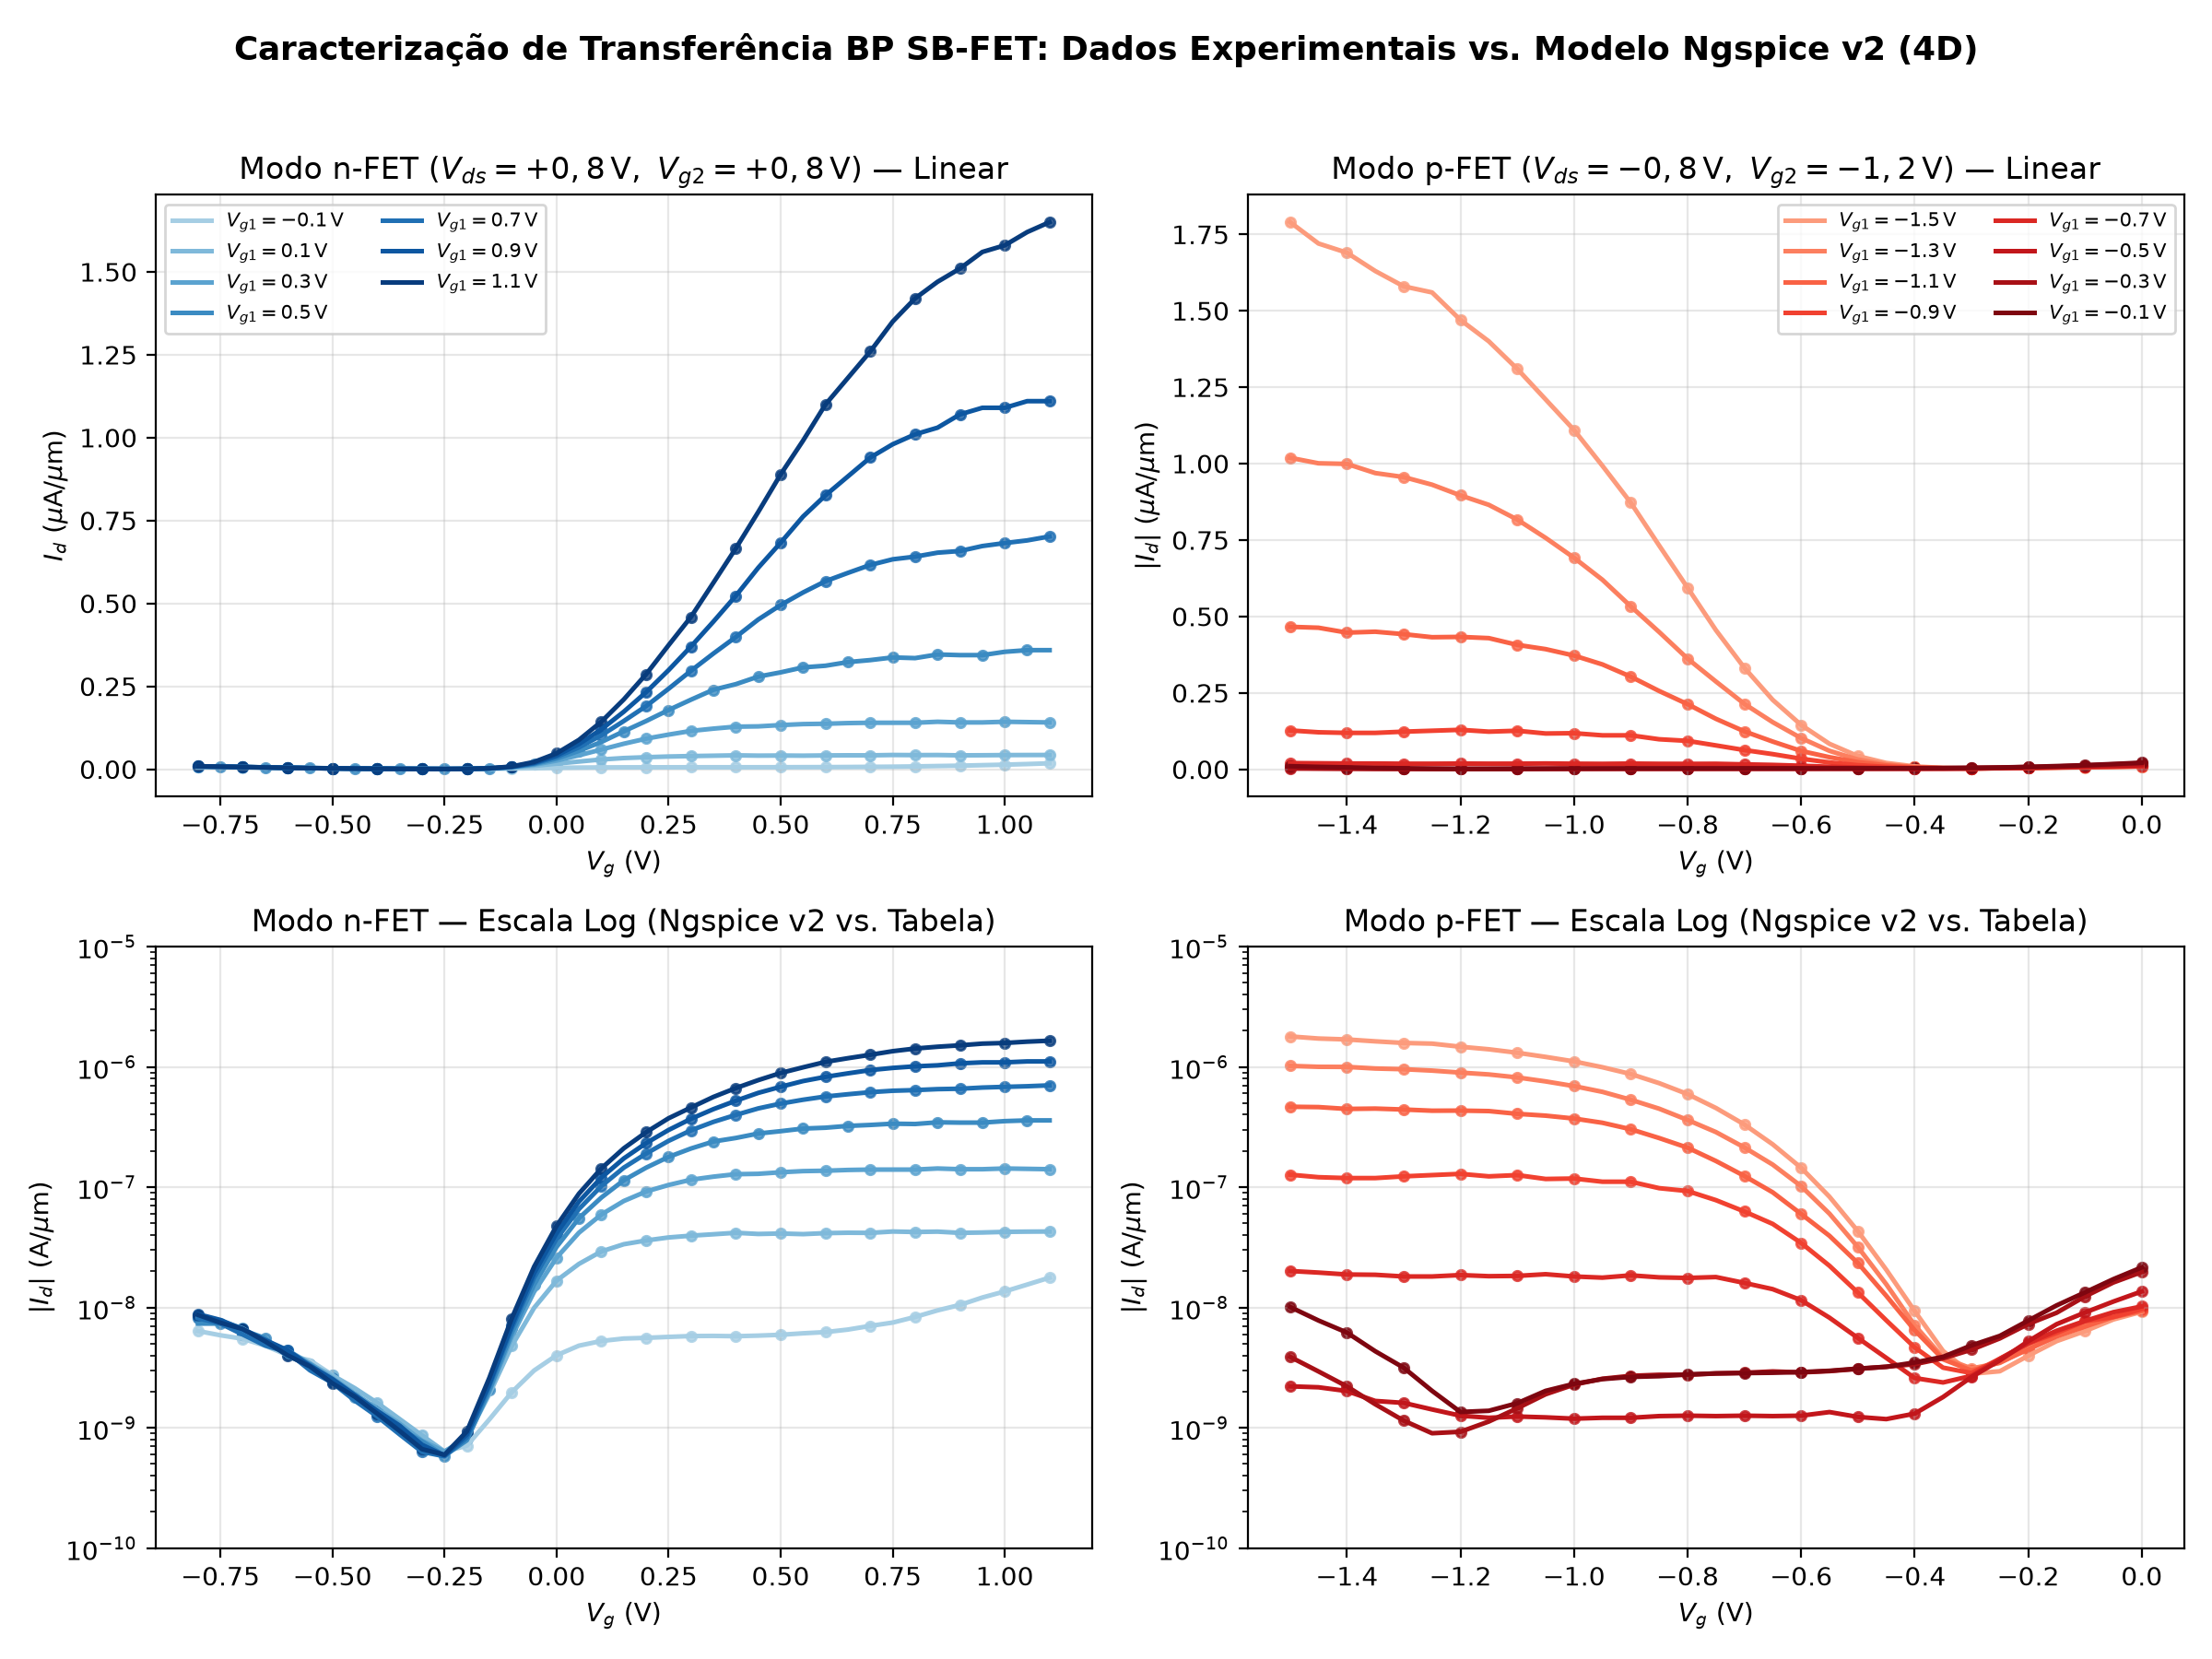
\includegraphics[width=0.92\textwidth]{m00_transfer_NP_log_lin.png}
\caption{Curvas de transfer\^{e}ncia ($I_d \times V_g$) em escalas linear e logar\'{i}tmica no \texttt{ngspice-47} comparadas aos pontos experimentais para os modos \textit{n-FET} e \textit{p-FET}.}
\label{fig:m00_transfer}
\end{figure}

\begin{figure}[htbp]
\centering
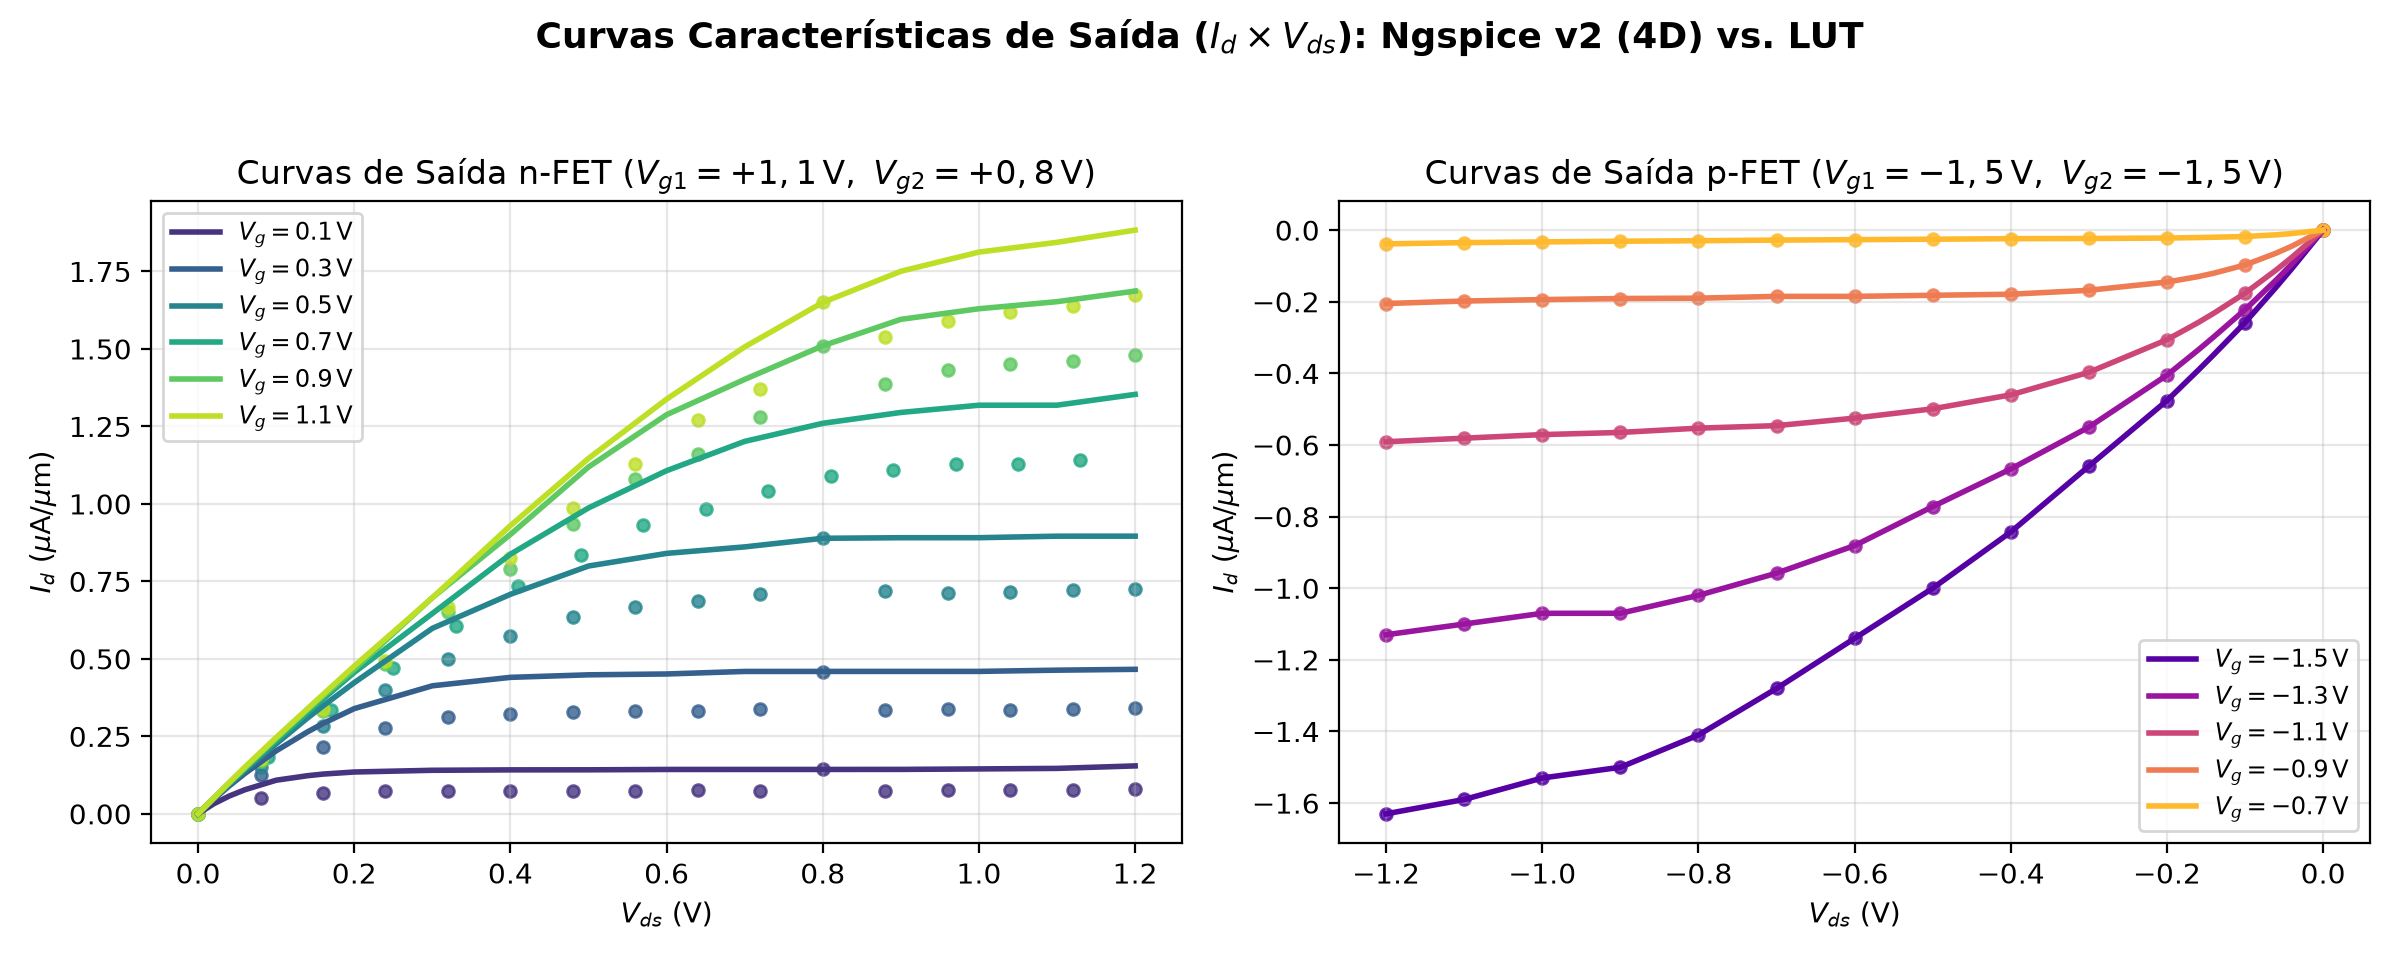
\includegraphics[width=0.92\textwidth]{m00_output_NP.png}
\caption{Fam\'{i}lias de curvas de sa\'{i}da ($I_d \times V_{ds}$) nos regimes \textit{n-FET} ($V_{ds}>0$) e \textit{p-FET} ($V_{ds}<0$, $V_{g2}=-1{,}5\ \text{V}$) reproduzindo a transi\c{c}\~{a}o tr\'{i}odo-satura\c{c}\~{a}o por porta.}
\label{fig:m00_output}
\end{figure}

\begin{figure}[htbp]
\centering
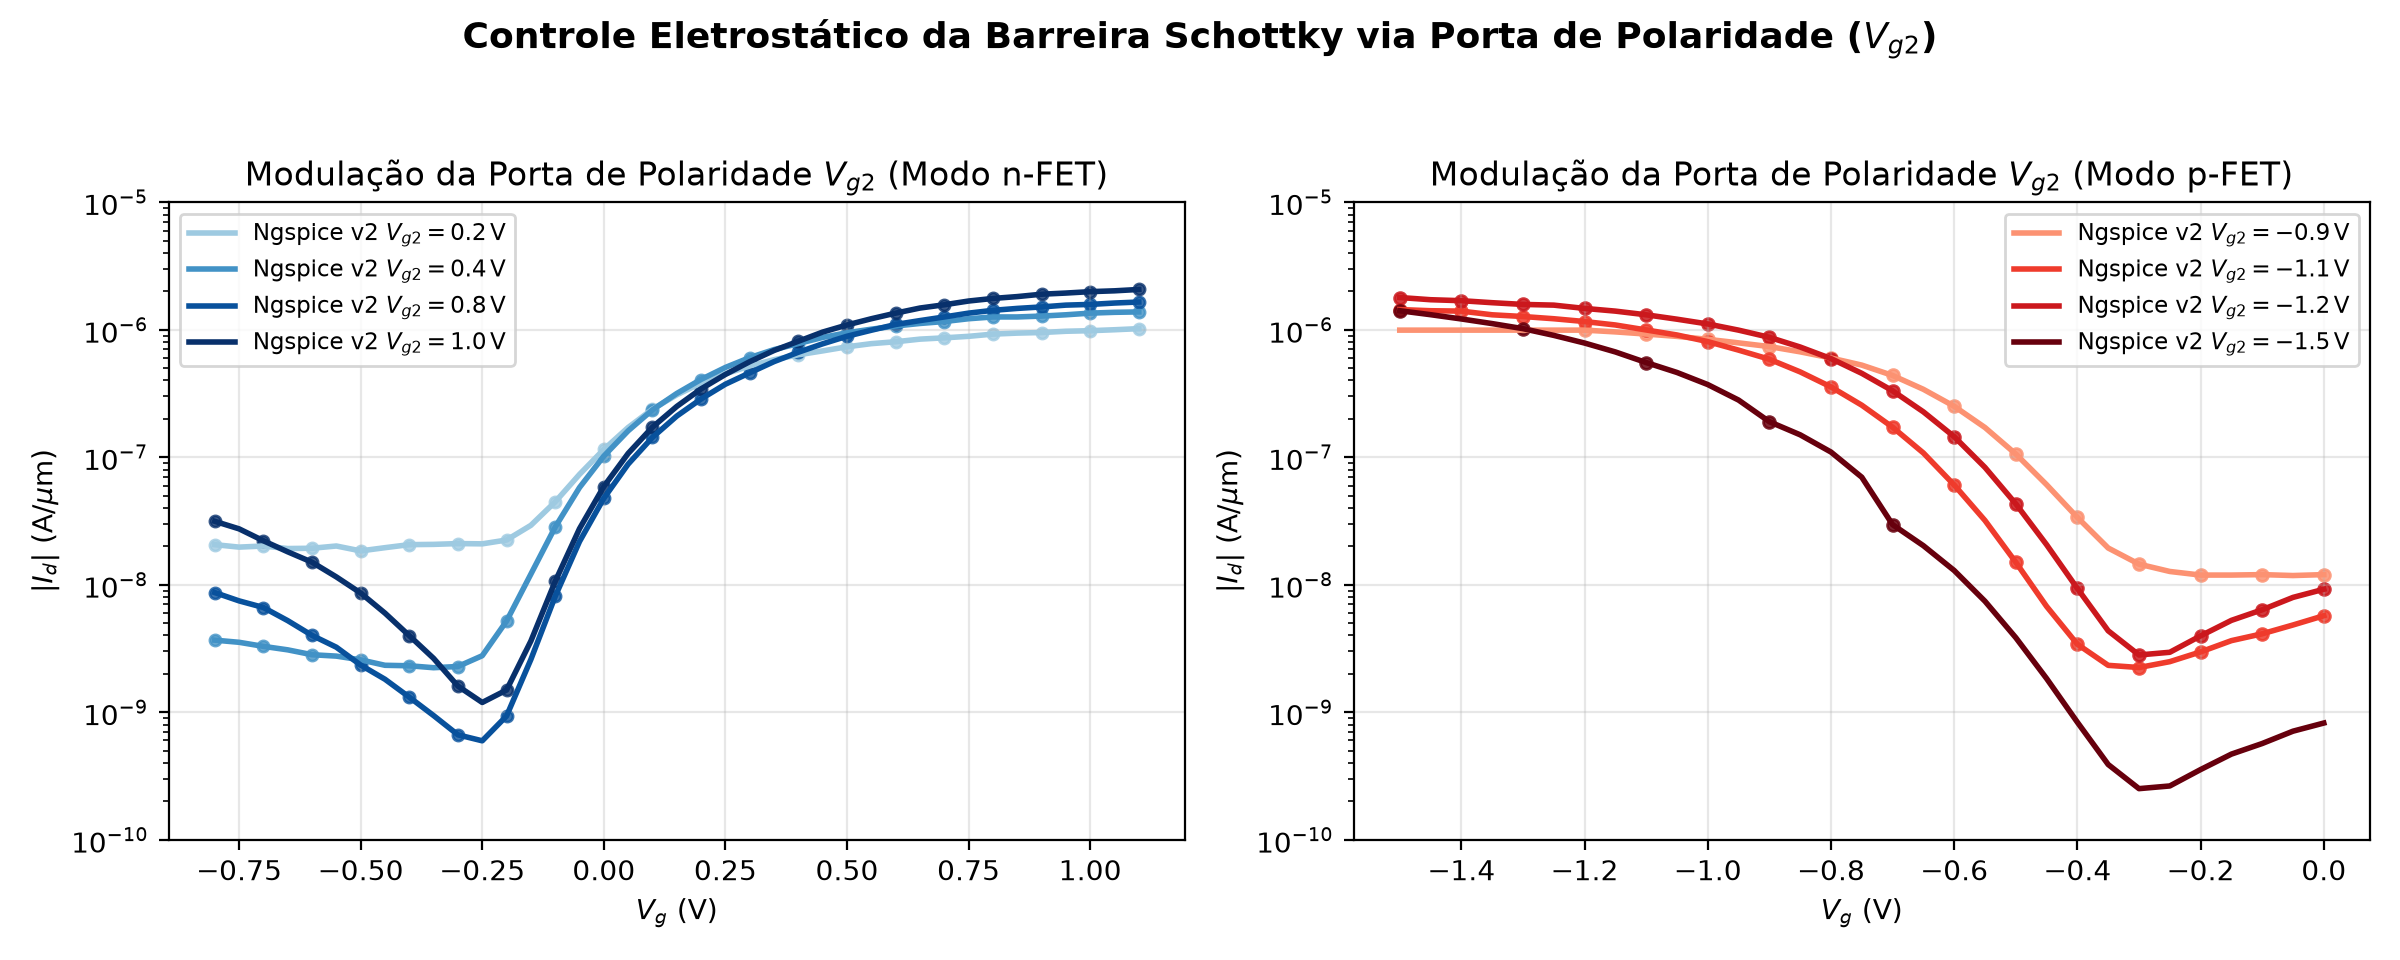
\includegraphics[width=0.92\textwidth]{m00_efeito_porta_polaridade.png}
\caption{Modula\c{c}\~{a}o eletrost\'{a}tica da porta de polaridade $V_{g2}$ sobre a corrente de canal no \textit{n-FET} e \textit{p-FET}, destacando o deslocamento de banda plana em $V_{g2}=-1{,}5\ \text{V}$.}
\label{fig:m00_pg}
\end{figure}

\begin{figure}[htbp]
\centering
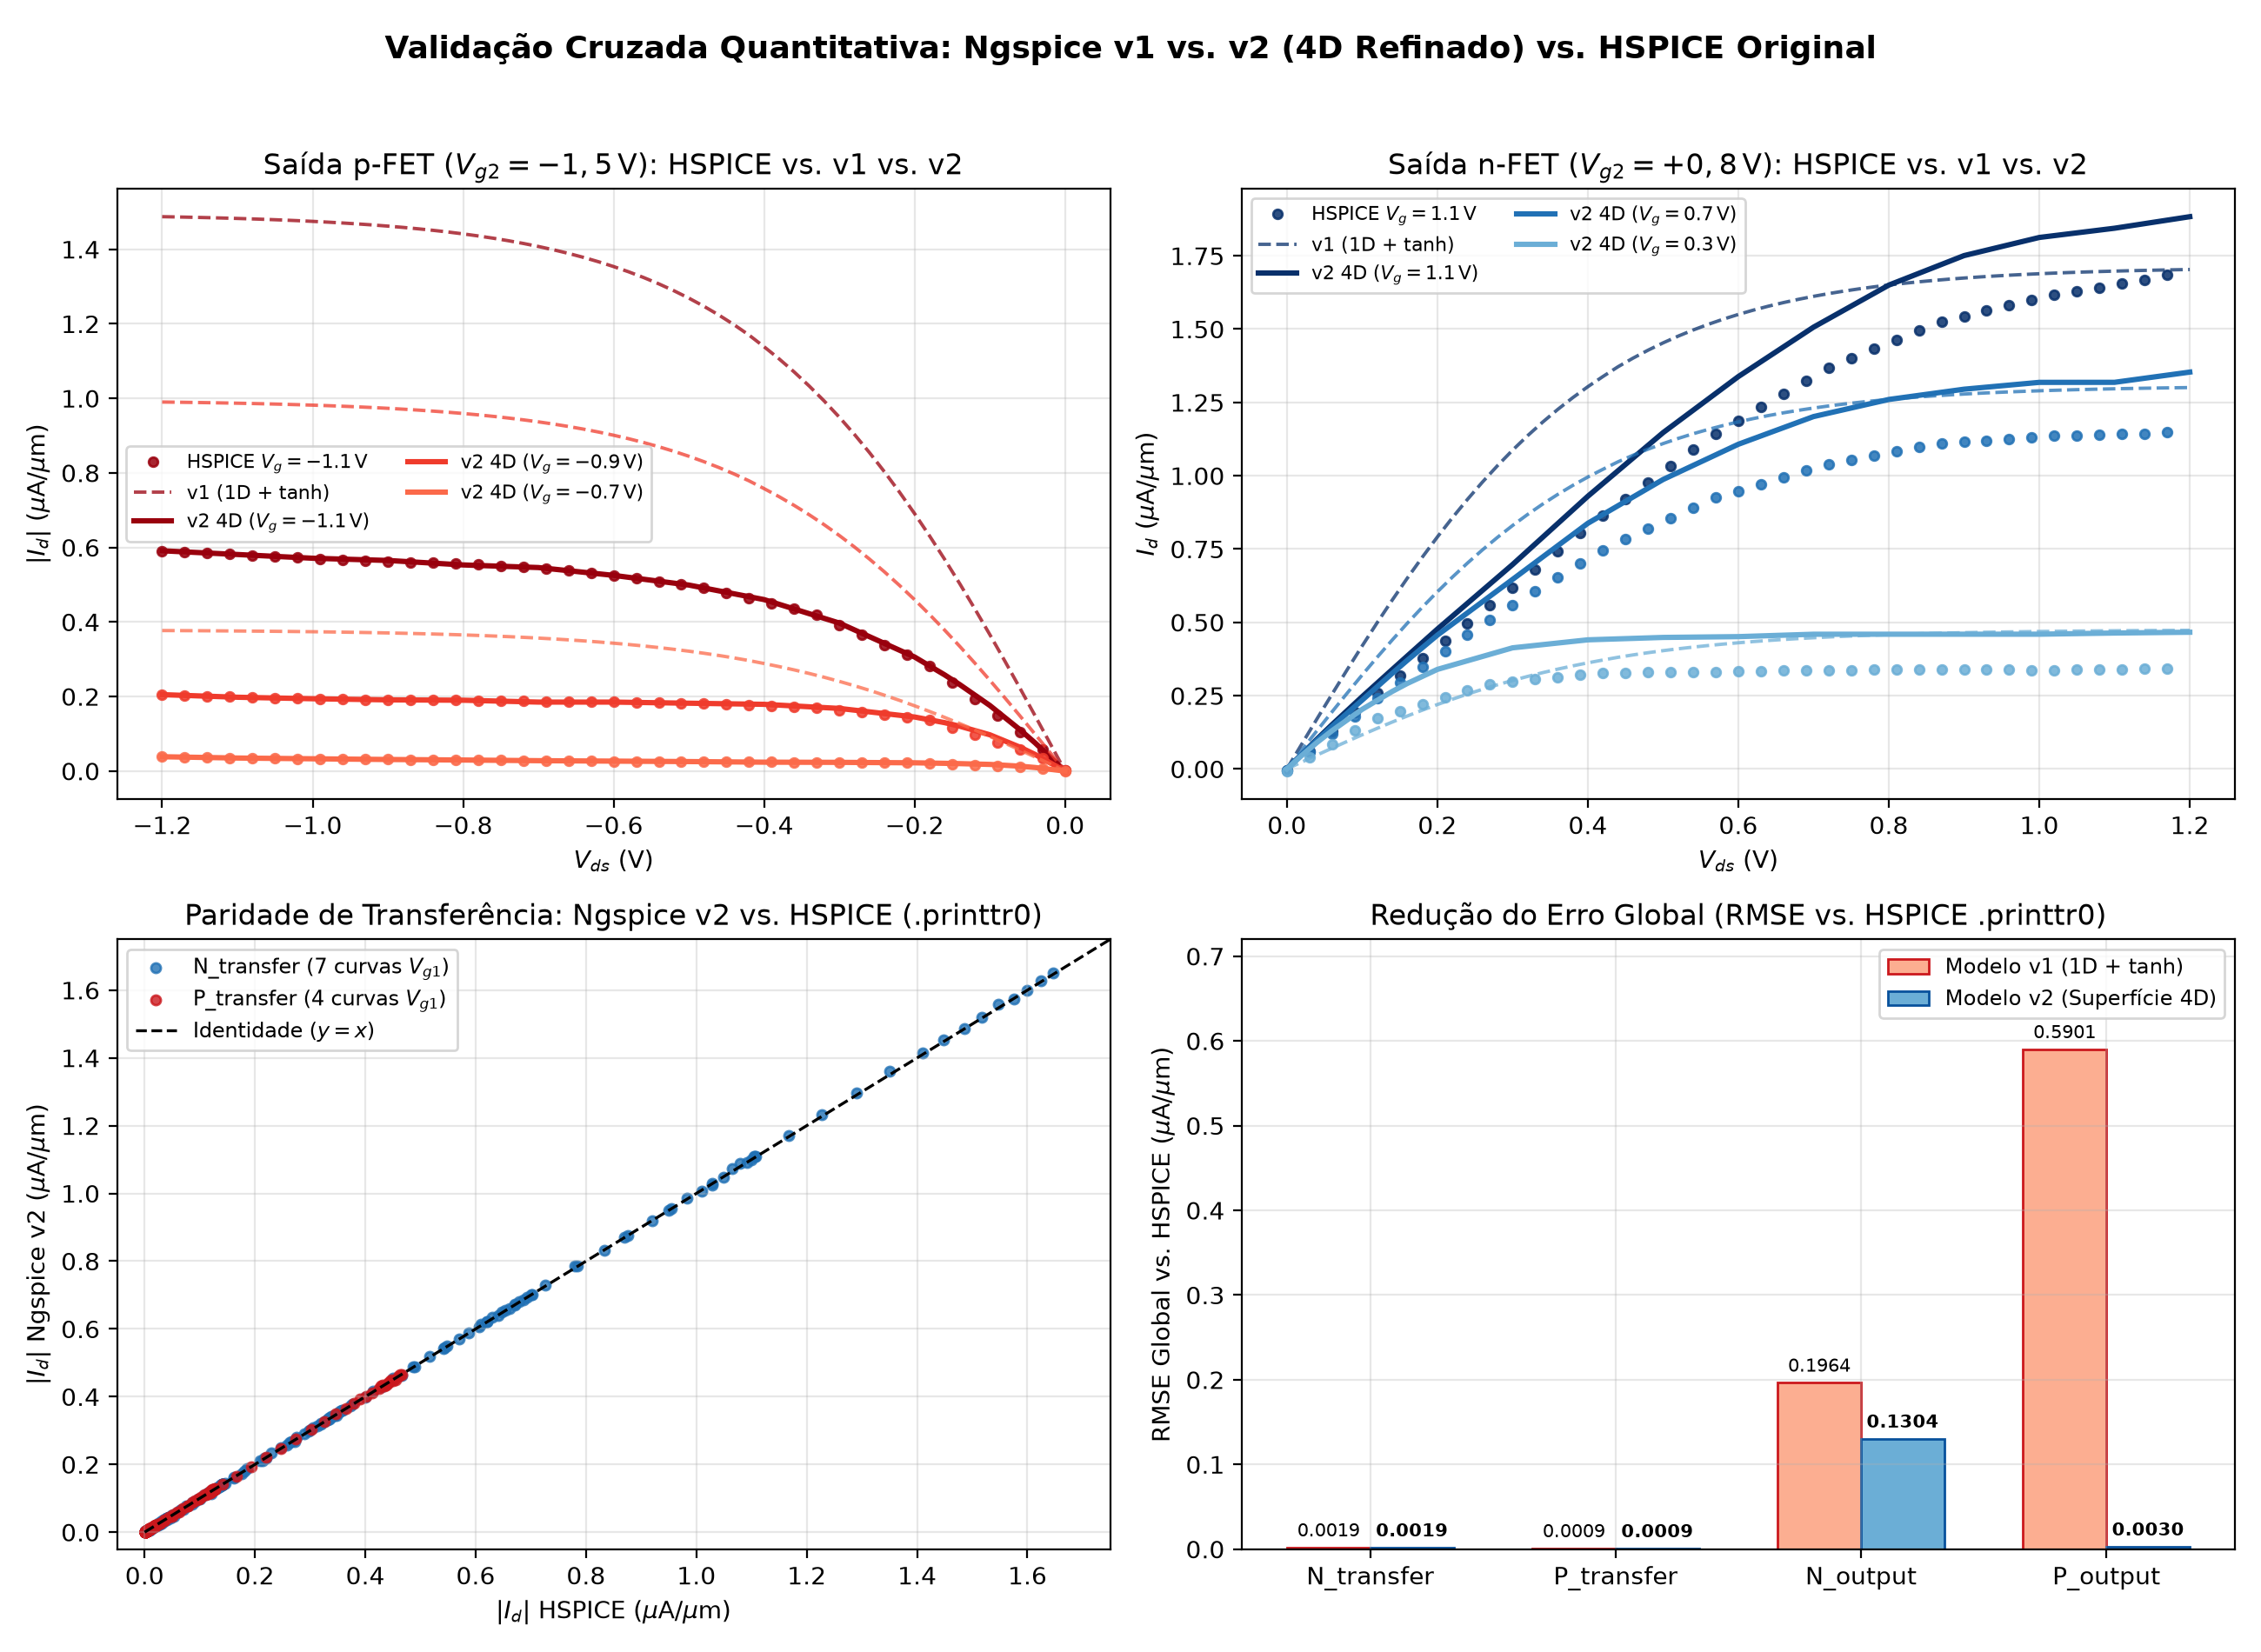
\includegraphics[width=0.92\textwidth]{m00_validacao_cruzada_hspice.png}
\caption{Valida\c{c}\~{a}o cruzada quantitativa entre o modelo preliminar (\texttt{v1}), o modelo 4D refinado (\texttt{v2}) no \texttt{ngspice-47} e as sa\'{i}das de refer\^{e}ncia \texttt{.printtr0} do Synopsys HSPICE.}
\label{fig:m00_hspice}
\end{figure}

\subsection{Inversor Complementar em Ultra-Baixa Tens\~{a}o}\label{sec:res_inversor}

Os resultados est\'{a}ticos do inversor complementar BP SB-FET entre $V_{DD} = 1{,}0\ \text{V}$ e $0{,}2\ \text{V}$ est\~{a}o compilados na Tabela~\ref{tab:inversor_vtc}. Sem compensa\c{c}\~{a}o de $V_{fb}$ (acoplamento direto), o desalinhamento entre os limiares dos ramos \textit{p-FET} e \textit{n-FET} desloca a tens\~{a}o de invers\~{a}o $V_M$ para pr\'{o}ximo de $0\ \text{V}$, colapsando completamente a fun\c{c}\~{a}o inversora em $V_{DD} \le 0{,}4\ \text{V}$ (excurs\~{a}o de $2{,}77\%$ e $|A_v|_{\max} = 0{,}37$ em $0{,}4\ \text{V}$; excurs\~{a}o de $1{,}27\%$ e ganho $0{,}06$ em $0{,}2\ \text{V}$).

\begin{table}[htbp]
\centering
\caption{M\'{e}tricas est\'{a}ticas do inversor complementar BP SB-FET sob escalonamento de $V_{DD}$ ($1{,}0\ \text{V}$ a $0{,}2\ \text{V}$).}
\label{tab:inversor_vtc}
\resizebox{\textwidth}{!}{%
\begin{tabular}{l c c c c c c c c}
\toprule
\textbf{Configura\c{c}\~{a}o} & $V_{DD}$ (V) & $V_{\mathrm{out}}(0)$ (V) & $V_{\mathrm{out}}(V_{DD})$ (V) & \textbf{Excurs\~{a}o (\%)} & $V_M$ (V) & $|A_v|_{\max}$ & $NM_L$ (V) & $NM_H$ (V) \\
\midrule
Direto (Sem comp.\ $V_{fb}$) & $1{,}0$ & $0{,}991$ & $0{,}004$ & $98{,}67\%$ & $0{,}278$ & $22{,}03$ & $0{,}096$ & $0{,}564$ \\
Direto (Sem comp.\ $V_{fb}$) & $0{,}8$ & $0{,}788$ & $0{,}004$ & $98{,}12\%$ & $0{,}162$ & $39{,}32$ & $0{,}034$ & $0{,}537$ \\
Direto (Sem comp.\ $V_{fb}$) & $0{,}6$ & $0{,}559$ & $0{,}003$ & $92{,}68\%$ & $0{,}066$ & $37{,}24$ & $0{,}000$ & $0{,}475$ \\
Direto (Sem comp.\ $V_{fb}$) & $0{,}4$ & $0{,}014$ & $0{,}003$ & $2{,}77\%$  & $0{,}010$ & $0{,}37$  & $0{,}000$ & $0{,}000$ \\
Direto (Sem comp.\ $V_{fb}$) & $0{,}2$ & $0{,}005$ & $0{,}003$ & $1{,}27\%$  & $0{,}006$ & $0{,}06$  & $0{,}000$ & $0{,}000$ \\
\midrule
Compensado ($V_{fb}$ alinhado) & $1{,}0$ & $0{,}999$ & $0{,}003$ & $99{,}63\%$ & $0{,}540$ & $54{,}69$ & $0{,}461$ & $0{,}373$ \\
Compensado ($V_{fb}$ alinhado) & $0{,}8$ & $0{,}800$ & $0{,}002$ & $99{,}75\%$ & $0{,}438$ & $50{,}84$ & $0{,}362$ & $0{,}278$ \\
Compensado ($V_{fb}$ alinhado) & $0{,}6$ & $0{,}600$ & $0{,}001$ & $99{,}80\%$ & $0{,}336$ & $38{,}18$ & $0{,}266$ & $0{,}178$ \\
Compensado ($V_{fb}$ alinhado) & $0{,}4$ & $0{,}400$ & $0{,}003$ & $99{,}29\%$ & $0{,}234$ & $12{,}71$ & $0{,}172$ & $0{,}076$ \\
Compensado ($V_{fb}$ alinhado) & $0{,}2$ & $0{,}198$ & $0{,}018$ & $89{,}75\%$ & $0{,}126$ & $2{,}71$  & $0{,}080$ & $0{,}000$ \\
\bottomrule
\end{tabular}}
\end{table}

Com o alinhamento eletrost\'{a}tico de $V_{fb}$, a tens\~{a}o de invers\~{a}o centraliza-se pr\'{o}ximo a $V_{DD}/2$ (Figura~\ref{fig:m01_vtc}), sustentando excurs\~{a}o superior a $99{,}2\%$ de $1{,}0\ \text{V}$ at\'{e} $0{,}4\ \text{V}$ e atingindo pico de ganho $|A_v|_{\max} = 54{,}69$ ($1{,}0\ \text{V}$) e $38{,}18$ ($0{,}6\ \text{V}$). Mesmo no regime extremo de ultra-baixa tens\~{a}o ($V_{DD} = 0{,}2\ \text{V}$), o inversor preserva excurs\~{a}o de $89{,}75\%$ e ganho diferencial de $2{,}71 > 1$, condição necess\'{a}ria para regenera\c{c}\~{a}o l\'{o}gica. Em regime transiente sob $C_{\mathrm{load}} = 0{,}5\ \text{fF}$ (Figura~\ref{fig:m01_tran}), as transi\c{c}\~{o}es ocorrem na escala de nanossegundos com corrente est\'{a}tica na ordem de nanoamperes e picos din\^{a}micos de $1{,}28\ \mu\text{A}$ em $1{,}0\ \text{V}$ e $0{,}73\ \mu\text{A}$ em $0{,}6\ \text{V}$.

\begin{figure}[htbp]
\centering
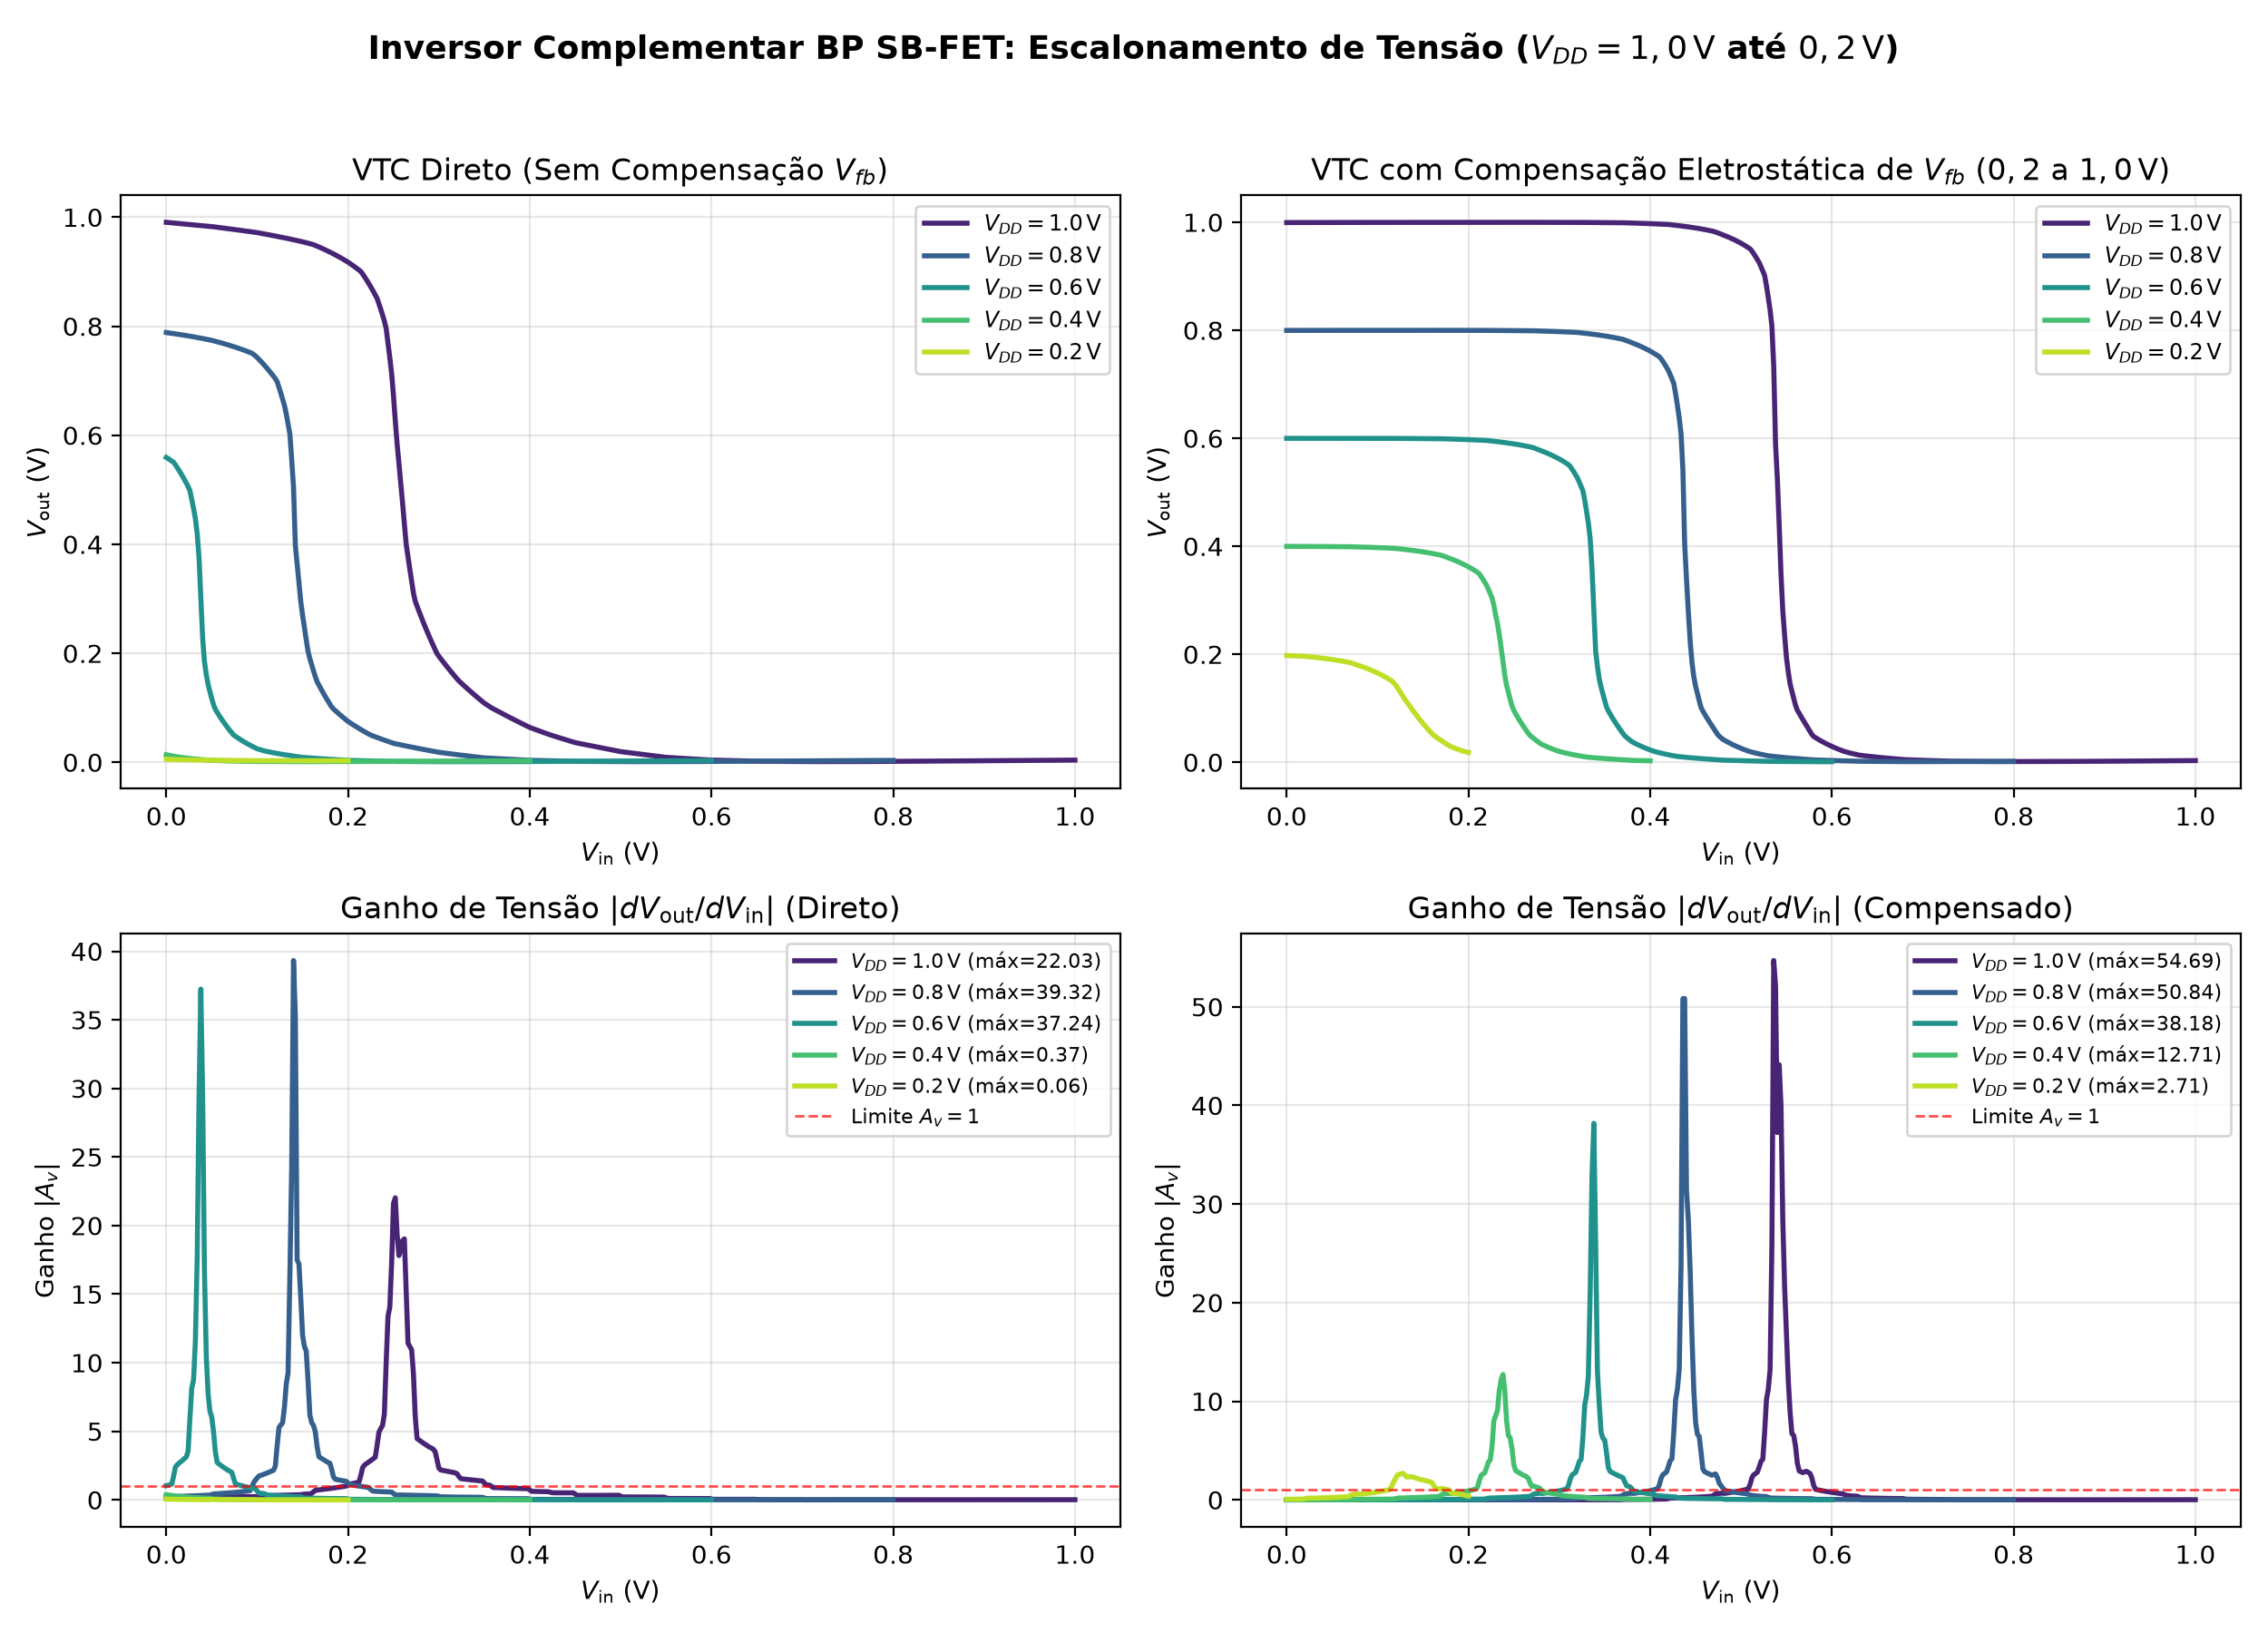
\includegraphics[width=0.92\textwidth]{m01_inversor_vtc_ganho.png}
\caption{Curvas de transfer\^{e}ncia de tens\~{a}o (VTC) e ganho diferencial $|dV_{\mathrm{out}}/dV_{\mathrm{in}}|$ do inversor BP SB-FET sem compensa\c{c}\~{a}o (esquerda) e com alinhamento de $V_{fb}$ (direita) de $1{,}0\ \text{V}$ a $0{,}2\ \text{V}$.}
\label{fig:m01_vtc}
\end{figure}

\begin{figure}[htbp]
\centering
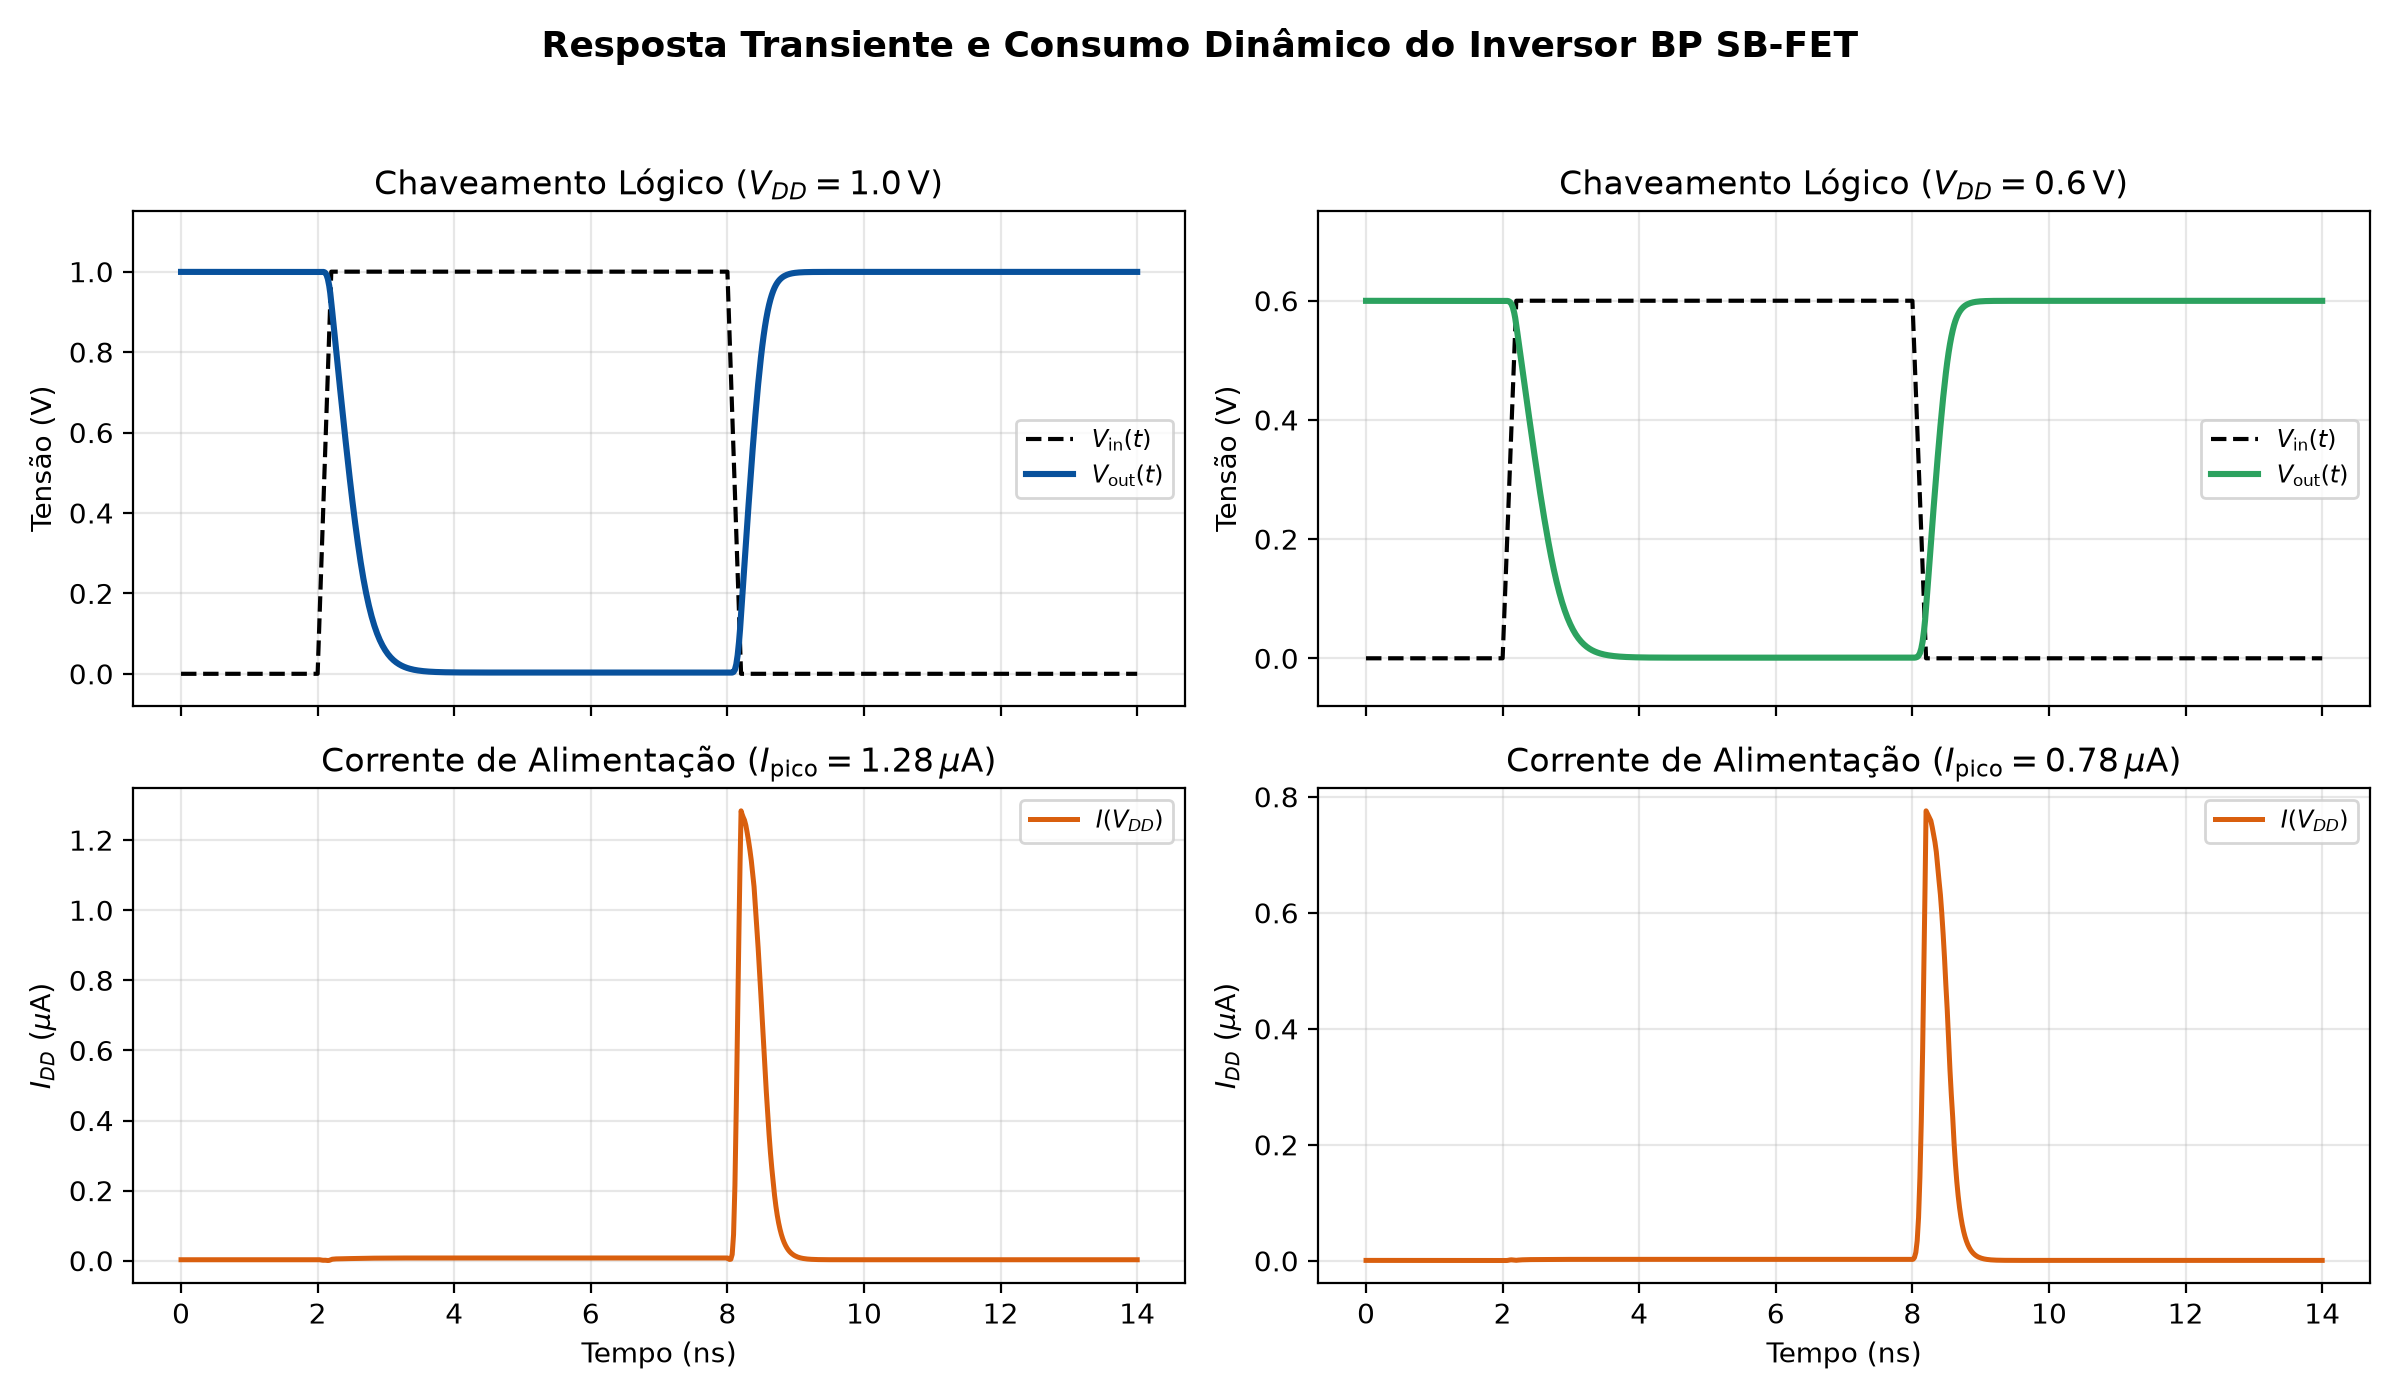
\includegraphics[width=0.90\textwidth]{m01_inversor_transiente.png}
\caption{Resposta transiente de chaveamento ($C_{\mathrm{load}} = 0{,}5\ \text{fF}$) e picos de corrente din\^{a}mica $I(V_{DD})$ do inversor compensado em $V_{DD} = 1{,}0\ \text{V}$ e $0{,}6\ \text{V}$.}
\label{fig:m01_tran}
\end{figure}

\subsection{Portas L\'{o}gicas Polim\'{o}rficas Din\^{a}micas (\texttt{NAND}/\texttt{NOR} e \texttt{XOR}/\texttt{XNOR})}\label{sec:res_poli}

As simula\c{c}\~{o}es transientes de $40\ \text{ns}$ comprovaram exatid\~{a}o booleana de $100\%$ ($16/16$ combina\c{c}\~{o}es de entrada e chave) em ambas as primitivas polim\'{o}rficas de 4 transistores sem sobrecarga de \'{a}rea, conforme detalhado na Tabela~\ref{tab:portas_polimorficas}. Na c\'{e}lula \texttt{NAND}/\texttt{NOR} ($V_{DD}=0{,}8\ \text{V}$), os n\'{i}veis l\'{o}gicos \texttt{'1'} situam-se entre $0{,}701\ \text{V}$ e $0{,}790\ \text{V}$, enquanto os n\'{i}veis \texttt{'0'} permanecem abaixo de $0{,}013\ \text{V}$. Na ponte \texttt{XOR}/\texttt{XNOR} ($V_{DD}=1{,}5\ \text{V}$, $V_{\mathrm{in}}=1{,}1\ \text{V}$), todos os estados \texttt{'1'} atingem exatamente $1{,}465\ \text{V}$ e todos os estados \texttt{'0'} estabilizam em $0{,}002\ \text{V}$.

\begin{table}[htbp]
\centering
\caption{Tabela-verdade el\'{e}trica e correntes de pico medidas no \texttt{ngspice-47} para as portas polim\'{o}rficas de 4T.}
\label{tab:portas_polimorficas}
\footnotesize
\begin{tabular}{l c c c c c c c}
\toprule
\textbf{Porta ($V_{DD}$)} & \textbf{Chave} & \textbf{Fun\c{c}\~{a}o} & $(A,B)$ & $V_{\mathrm{out}}$ (V) & \textbf{Bit Med.} & \textbf{Bit Esp.} & $I_{\mathrm{pico}}$ ($\mu\text{A}$) \\
\midrule
\texttt{NAND}/\texttt{NOR} ($0{,}8\ \text{V}$) & $\text{Key}=0$ & \texttt{NAND} & \texttt{00} & $0{,}790$ & \texttt{1} & \texttt{1} & $0{,}041$ \\
\texttt{NAND}/\texttt{NOR} ($0{,}8\ \text{V}$) & $\text{Key}=0$ & \texttt{NAND} & \texttt{01} & $0{,}762$ & \texttt{1} & \texttt{1} & $0{,}182$ \\
\texttt{NAND}/\texttt{NOR} ($0{,}8\ \text{V}$) & $\text{Key}=0$ & \texttt{NAND} & \texttt{10} & $0{,}769$ & \texttt{1} & \texttt{1} & $0{,}390$ \\
\texttt{NAND}/\texttt{NOR} ($0{,}8\ \text{V}$) & $\text{Key}=0$ & \texttt{NAND} & \texttt{11} & $0{,}013$ & \texttt{0} & \texttt{0} & $0{,}589$ \\
\texttt{NAND}/\texttt{NOR} ($0{,}8\ \text{V}$) & $\text{Key}=1$ & \texttt{NOR}  & \texttt{00} & $0{,}701$ & \texttt{1} & \texttt{1} & $0{,}213$ \\
\texttt{NAND}/\texttt{NOR} ($0{,}8\ \text{V}$) & $\text{Key}=1$ & \texttt{NOR}  & \texttt{01} & $0{,}001$ & \texttt{0} & \texttt{0} & $0{,}716$ \\
\texttt{NAND}/\texttt{NOR} ($0{,}8\ \text{V}$) & $\text{Key}=1$ & \texttt{NOR}  & \texttt{10} & $0{,}004$ & \texttt{0} & \texttt{0} & $0{,}092$ \\
\texttt{NAND}/\texttt{NOR} ($0{,}8\ \text{V}$) & $\text{Key}=1$ & \texttt{NOR}  & \texttt{11} & $0{,}001$ & \texttt{0} & \texttt{0} & $0{,}006$ \\
\midrule
\texttt{XOR}/\texttt{XNOR} ($1{,}5\ \text{V}$) & $\text{Key}=0$ & \texttt{XOR}  & \texttt{00} & $0{,}002$ & \texttt{0} & \texttt{0} & $0{,}004$ \\
\texttt{XOR}/\texttt{XNOR} ($1{,}5\ \text{V}$) & $\text{Key}=0$ & \texttt{XOR}  & \texttt{01} & $1{,}465$ & \texttt{1} & \texttt{1} & $1{,}691$ \\
\texttt{XOR}/\texttt{XNOR} ($1{,}5\ \text{V}$) & $\text{Key}=0$ & \texttt{XOR}  & \texttt{10} & $1{,}465$ & \texttt{1} & \texttt{1} & $0{,}366$ \\
\texttt{XOR}/\texttt{XNOR} ($1{,}5\ \text{V}$) & $\text{Key}=0$ & \texttt{XOR}  & \texttt{11} & $0{,}002$ & \texttt{0} & \texttt{0} & $1{,}903$ \\
\texttt{XOR}/\texttt{XNOR} ($1{,}5\ \text{V}$) & $\text{Key}=1$ & \texttt{XNOR} & \texttt{00} & $1{,}465$ & \texttt{1} & \texttt{1} & $1{,}699$ \\
\texttt{XOR}/\texttt{XNOR} ($1{,}5\ \text{V}$) & $\text{Key}=1$ & \texttt{XNOR} & \texttt{01} & $0{,}002$ & \texttt{0} & \texttt{0} & $1{,}908$ \\
\texttt{XOR}/\texttt{XNOR} ($1{,}5\ \text{V}$) & $\text{Key}=1$ & \texttt{XNOR} & \texttt{10} & $0{,}002$ & \texttt{0} & \texttt{0} & $0{,}032$ \\
\texttt{XOR}/\texttt{XNOR} ($1{,}5\ \text{V}$) & $\text{Key}=1$ & \texttt{XNOR} & \texttt{11} & $1{,}465$ & \texttt{1} & \texttt{1} & $1{,}691$ \\
\bottomrule
\end{tabular}
\end{table}

As Figuras~\ref{fig:m02_nand_nor} e \ref{fig:m02_xor_xnor} evidenciam a transmuta\c{c}\~{a}o instant\^{a}nea em $t = 20\ \text{ns}$ e exp\~{o}em uma diferen\c{c}a estrutural fundamental: enquanto \texttt{NAND}/\texttt{NOR} apresenta picos de corrente fortemente dependentes da rede s\'{e}rie ou paralela que realiza a transi\c{c}\~{a}o, a ponte \texttt{XOR}/\texttt{XNOR} exibe picos de carga ($\approx 1{,}69\ \mu\text{A}$) e descarga ($\approx 1{,}90\text{--}1{,}91\ \mu\text{A}$) praticamente espelhados entre os dois modos de chave.

\begin{figure}[htbp]
\centering
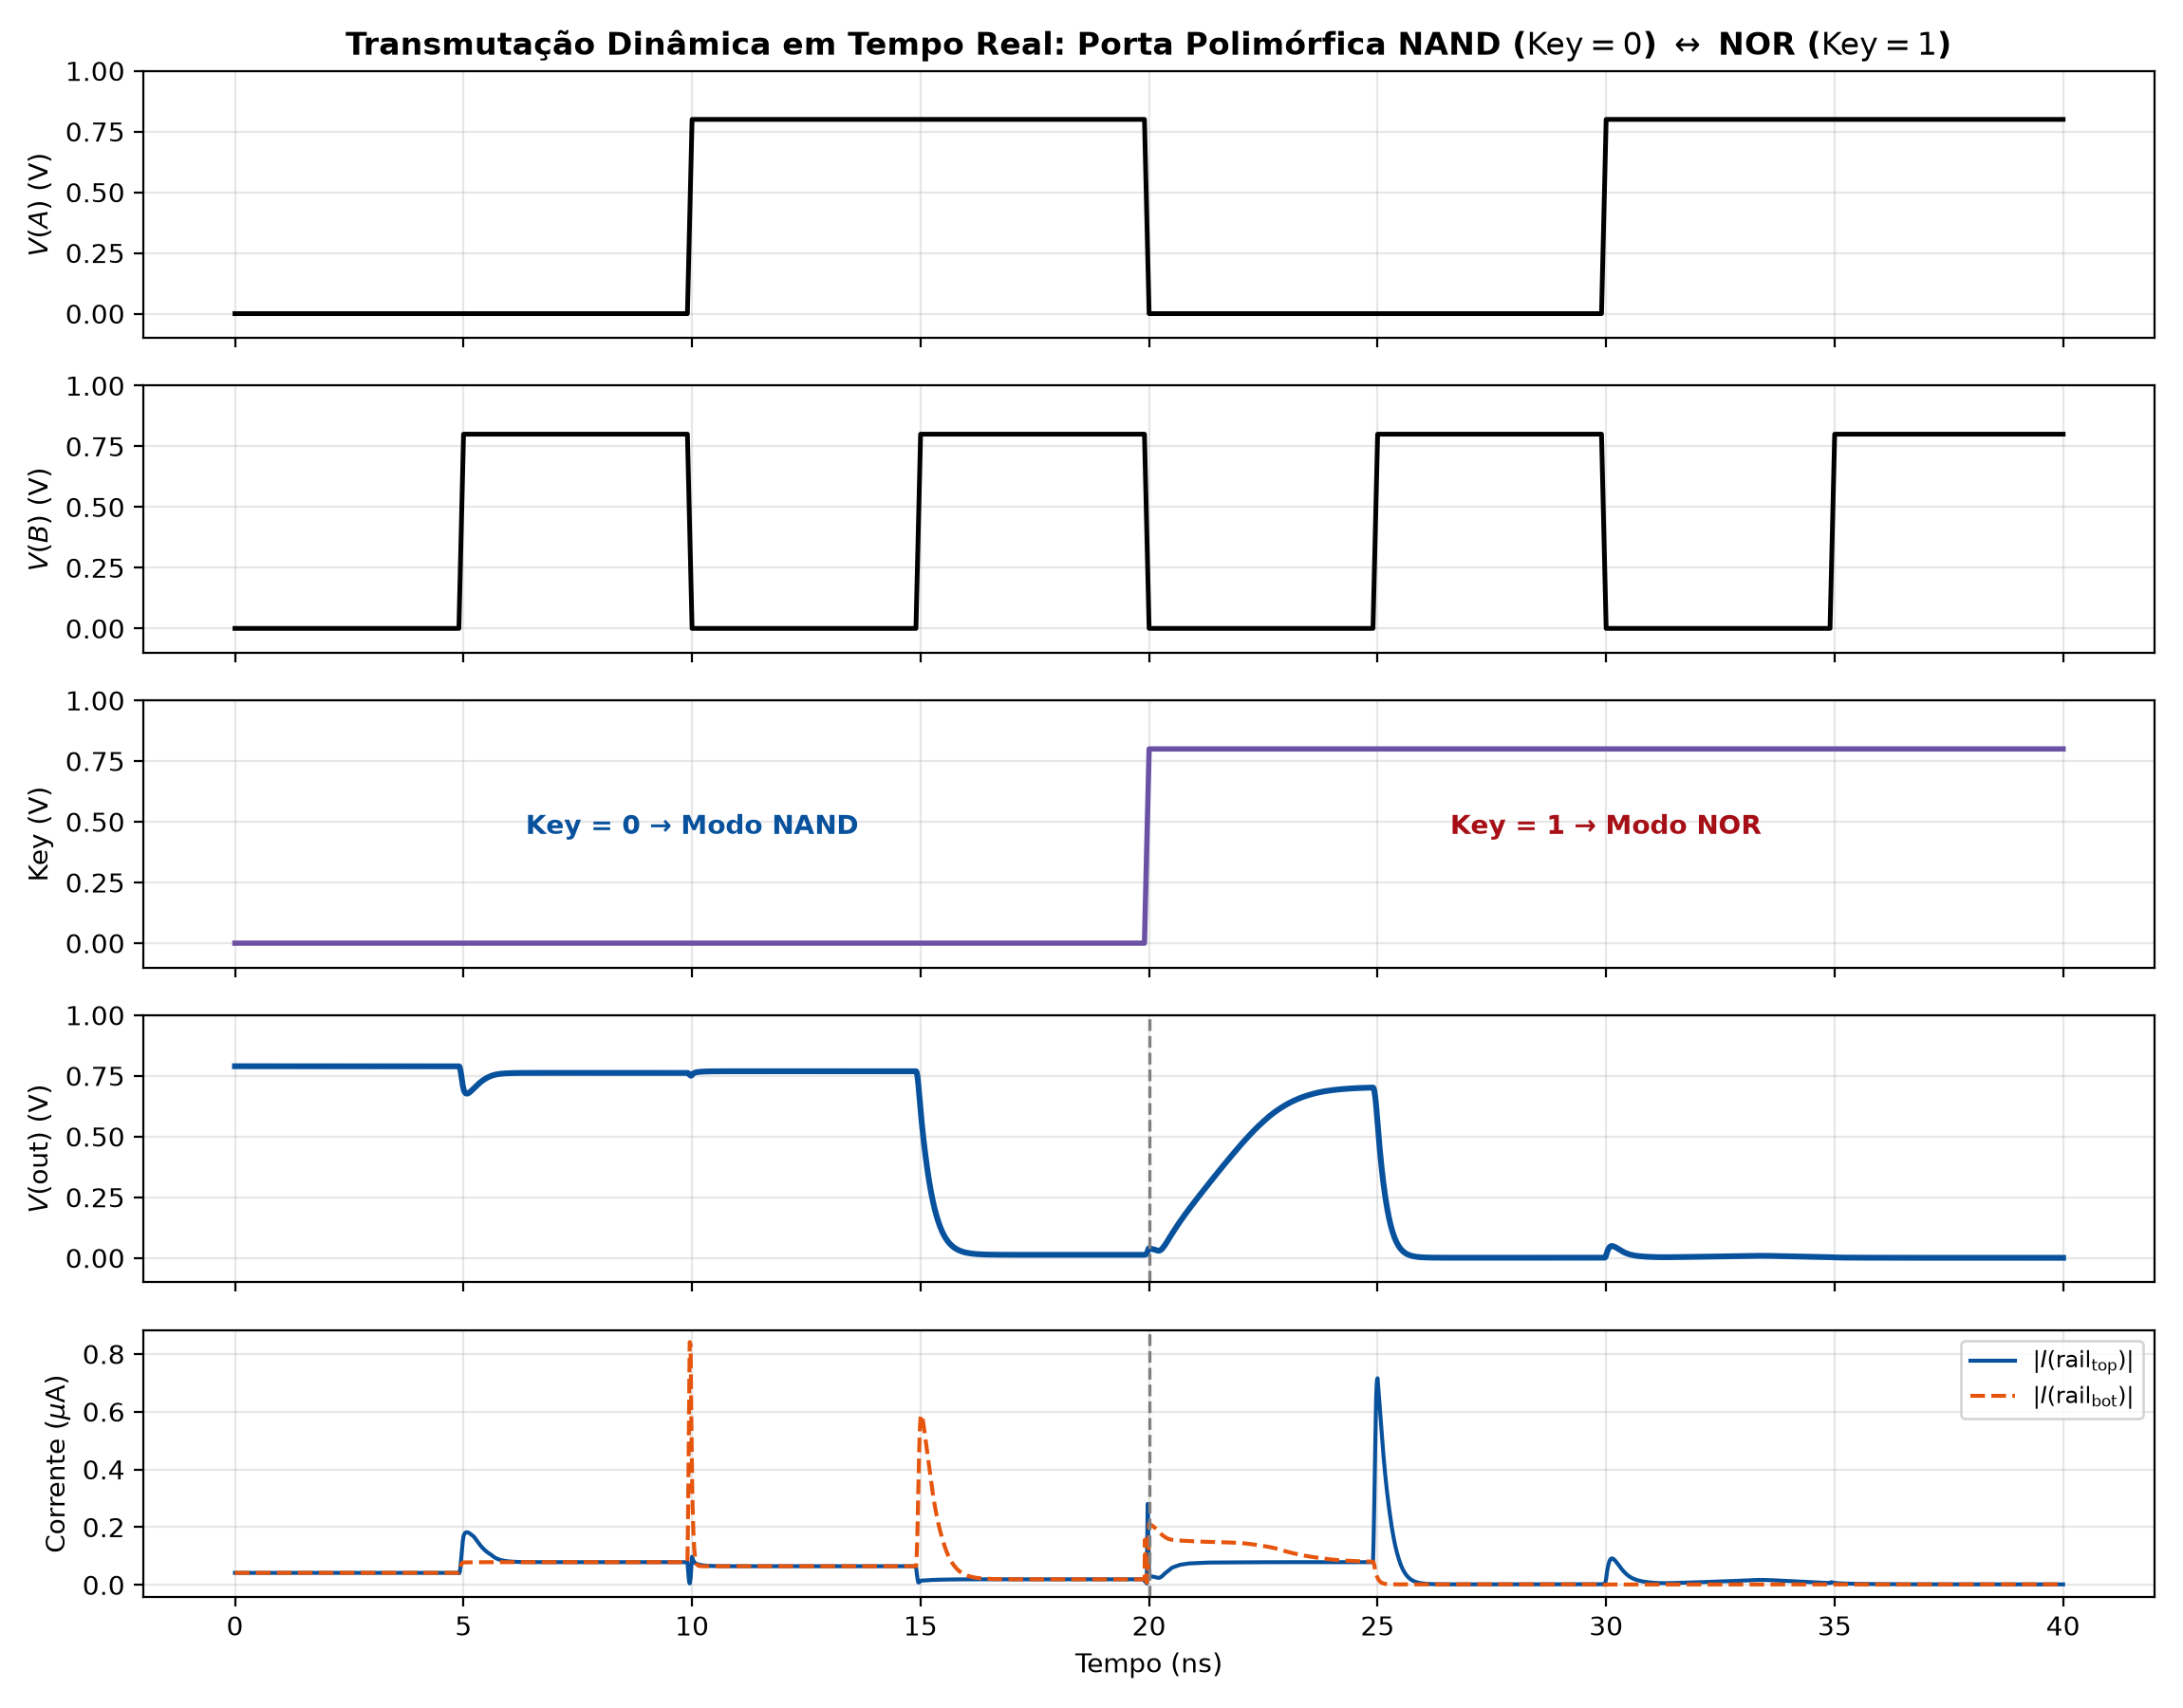
\includegraphics[width=0.90\textwidth]{m02_nand_nor_dinamico.png}
\caption{Comuta\c{c}\~{a}o din\^{a}mica \texttt{NAND} ($\text{Key}=0$) $\leftrightarrow$ \texttt{NOR} ($\text{Key}=1$) em $V_{DD} = 0{,}8\ \text{V}$ e perfil assim\'{e}trico da corrente de alimenta\c{c}\~{a}o.}
\label{fig:m02_nand_nor}
\end{figure}

\begin{figure}[htbp]
\centering
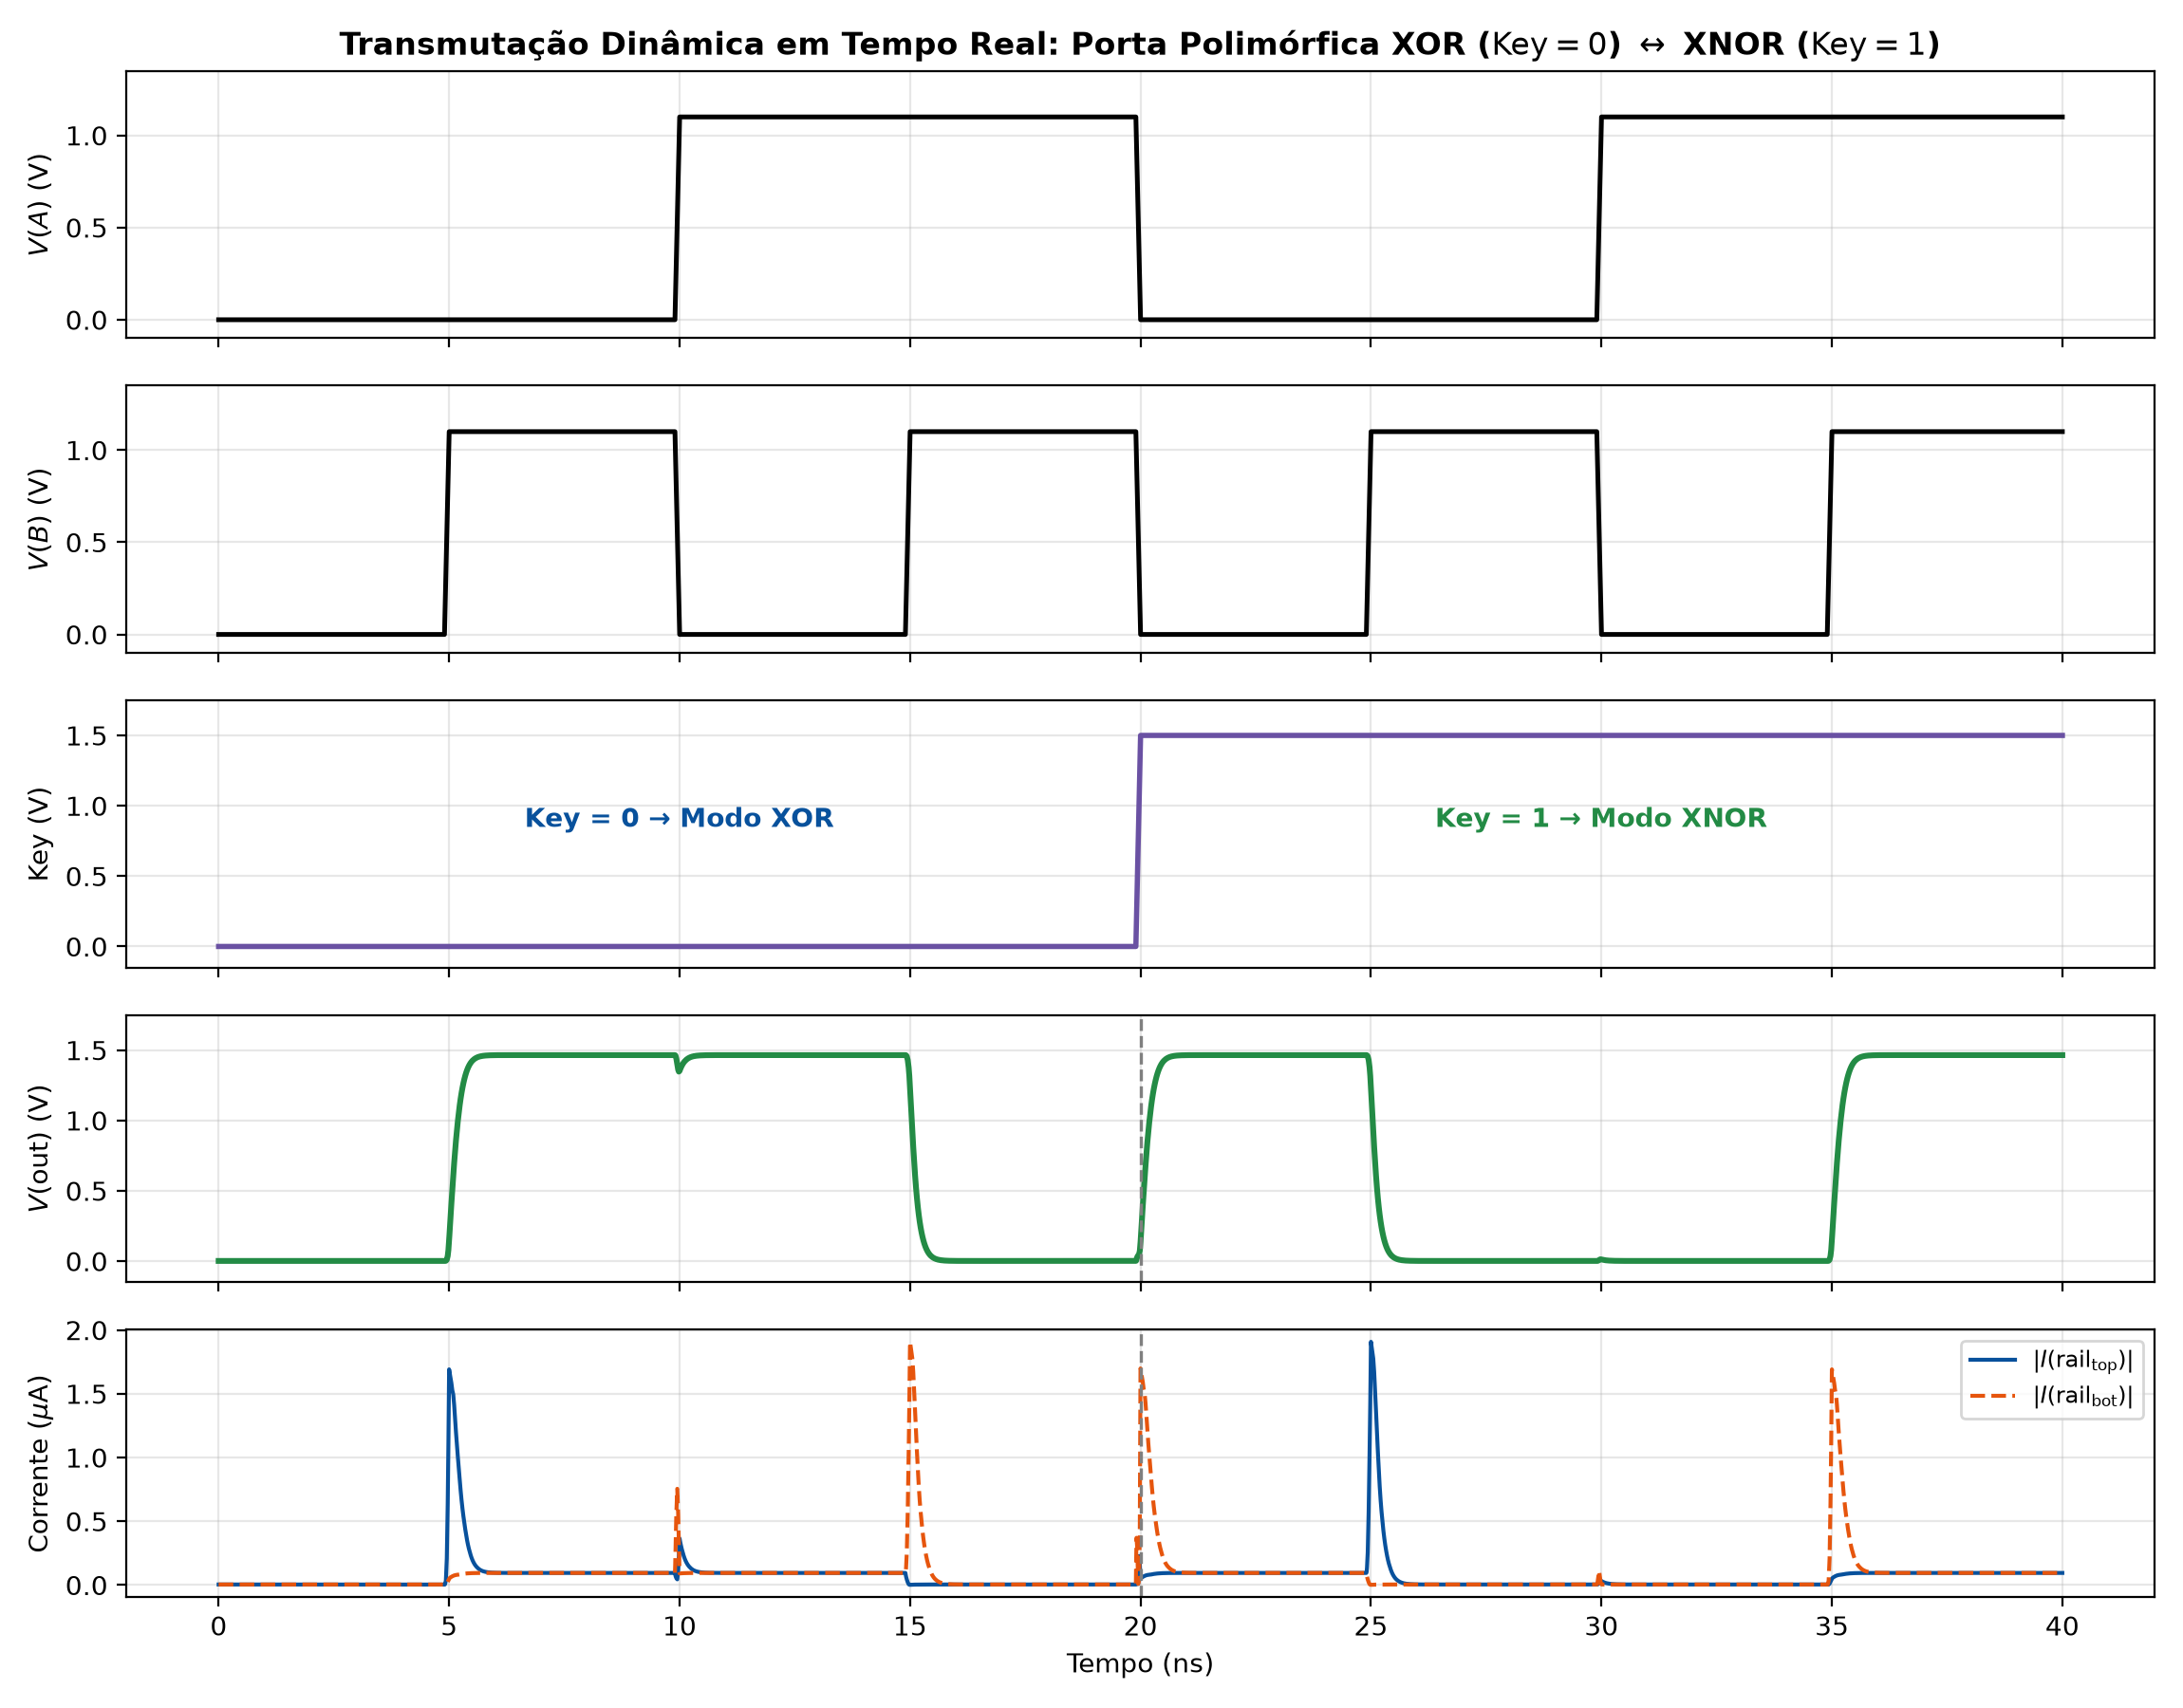
\includegraphics[width=0.90\textwidth]{m02_xor_xnor_dinamico.png}
\caption{Comuta\c{c}\~{a}o din\^{a}mica \texttt{XOR} ($\text{Key}=0$) $\leftrightarrow$ \texttt{XNOR} ($\text{Key}=1$) em $V_{DD} = 1{,}5\ \text{V}$ com simetria nos picos de chaveamento complementares.}
\label{fig:m02_xor_xnor}
\end{figure}

\subsection{Seguran\c{c}a contra Canal Lateral (DPA), Robustez 3D e Reten\c{c}\~{a}o Flutuante}\label{sec:res_dpa_mc}

A an\'{a}lise reproduzida em Python sobre as formas de onda experimentais de~\cite{wu2020reconfigurable} (Tabela~\ref{tab:dpa_mc_m03} e Figura~\ref{fig:m03_dpa}) confirma que a fam\'{i}lia \texttt{NAND}/\texttt{NOR} exibe uma discrep\^{a}ncia de $50{,}3\%$ nos picos de corrente ($2{,}15\ \mu\text{A}$ vs.\ $1{,}43\ \mu\text{A}$) e correla\c{c}\~{a}o temporal limitada ($r = 0{,}515$), enquanto a fam\'{i}lia \texttt{XOR}/\texttt{XNOR} reduz a diferen\c{c}a entre picos para apenas $0{,}56\%$ ($1{,}80\ \mu\text{A}$ vs.\ $1{,}79\ \mu\text{A}$), mascarando a identidade da chave sob monitoramento de canal lateral.

\begin{table}[htbp]
\centering
\caption{M\'{e}tricas de assinatura DPA e robustez estat\'{i}stica Monte Carlo ($N=250$ amostras/porta) do M\'{o}dulo \texttt{03}.}
\label{tab:dpa_mc_m03}
\begin{subtable}{\textwidth}
\centering
\caption{Compara\c{c}\~{a}o de assinaturas de corrente $|I(V_{DD})|$ entre modos (\texttt{metricas\_dpa.csv}).}
\footnotesize
\begin{tabular}{l c c c c c c}
\toprule
\textbf{Fam\'{i}lia} & $I_{\mathrm{pico},0}$ ($\mu\text{A}$) & $I_{\mathrm{pico},1}$ ($\mu\text{A}$) & \textbf{Dif.\ Pico (\%)} & $I_{\mathrm{m\acute{e}d},0}$ ($\mu\text{A}$) & $I_{\mathrm{m\acute{e}d},1}$ ($\mu\text{A}$) & \textbf{Correla\c{c}\~{a}o} $r$ \\
\midrule
\texttt{NAND}/\texttt{NOR} & $2{,}15$ & $1{,}43$ & $50{,}35\%$ & $0{,}212$ & $0{,}163$ & $+0{,}515$ \\
\texttt{XOR}/\texttt{XNOR} & $1{,}80$ & $1{,}79$ & $0{,}56\%$  & $0{,}267$ & $0{,}230$ & $-0{,}114$ \\
\bottomrule
\end{tabular}
\end{subtable}

\vspace{0.8em}

\begin{subtable}{\textwidth}
\centering
\caption{Estat\'{i}sticas de separa\c{c}\~{a}o l\'{o}gica sob ru\'{i}do simult\^{a}neo em $V_{DD}$ e $V_{SS}$ (\texttt{metricas\_seguranca\_robustez.csv}).}
\footnotesize
\begin{tabular}{l c c c c c c}
\toprule
\textbf{Porta} & \textbf{Amostras} & $\mu(V_{\text{`1'}})$ (V) & $\sigma(V_{\text{`1'}})$ (mV) & $\mu(V_{\text{`0'}})$ (V) & $\sigma(V_{\text{`0'}})$ (mV) & \textbf{Acerto L\'{o}gico} \\
\midrule
\texttt{NAND} & $250$ & $0{,}793$ & $126{,}55$ & $0{,}038$ & $106{,}50$ & $100{,}0\%$ \\
\texttt{NOR}  & $250$ & $0{,}770$ & $118{,}01$ & $0{,}015$ & $101{,}47$ & $100{,}0\%$ \\
\texttt{XOR}  & $250$ & $0{,}782$ & $122{,}80$ & $0{,}006$ & $89{,}23$  & $100{,}0\%$ \\
\texttt{XNOR} & $250$ & $0{,}782$ & $122{,}69$ & $0{,}006$ & $89{,}05$  & $100{,}0\%$ \\
\bottomrule
\end{tabular}
\end{subtable}
\end{table}

\begin{figure}[htbp]
\centering
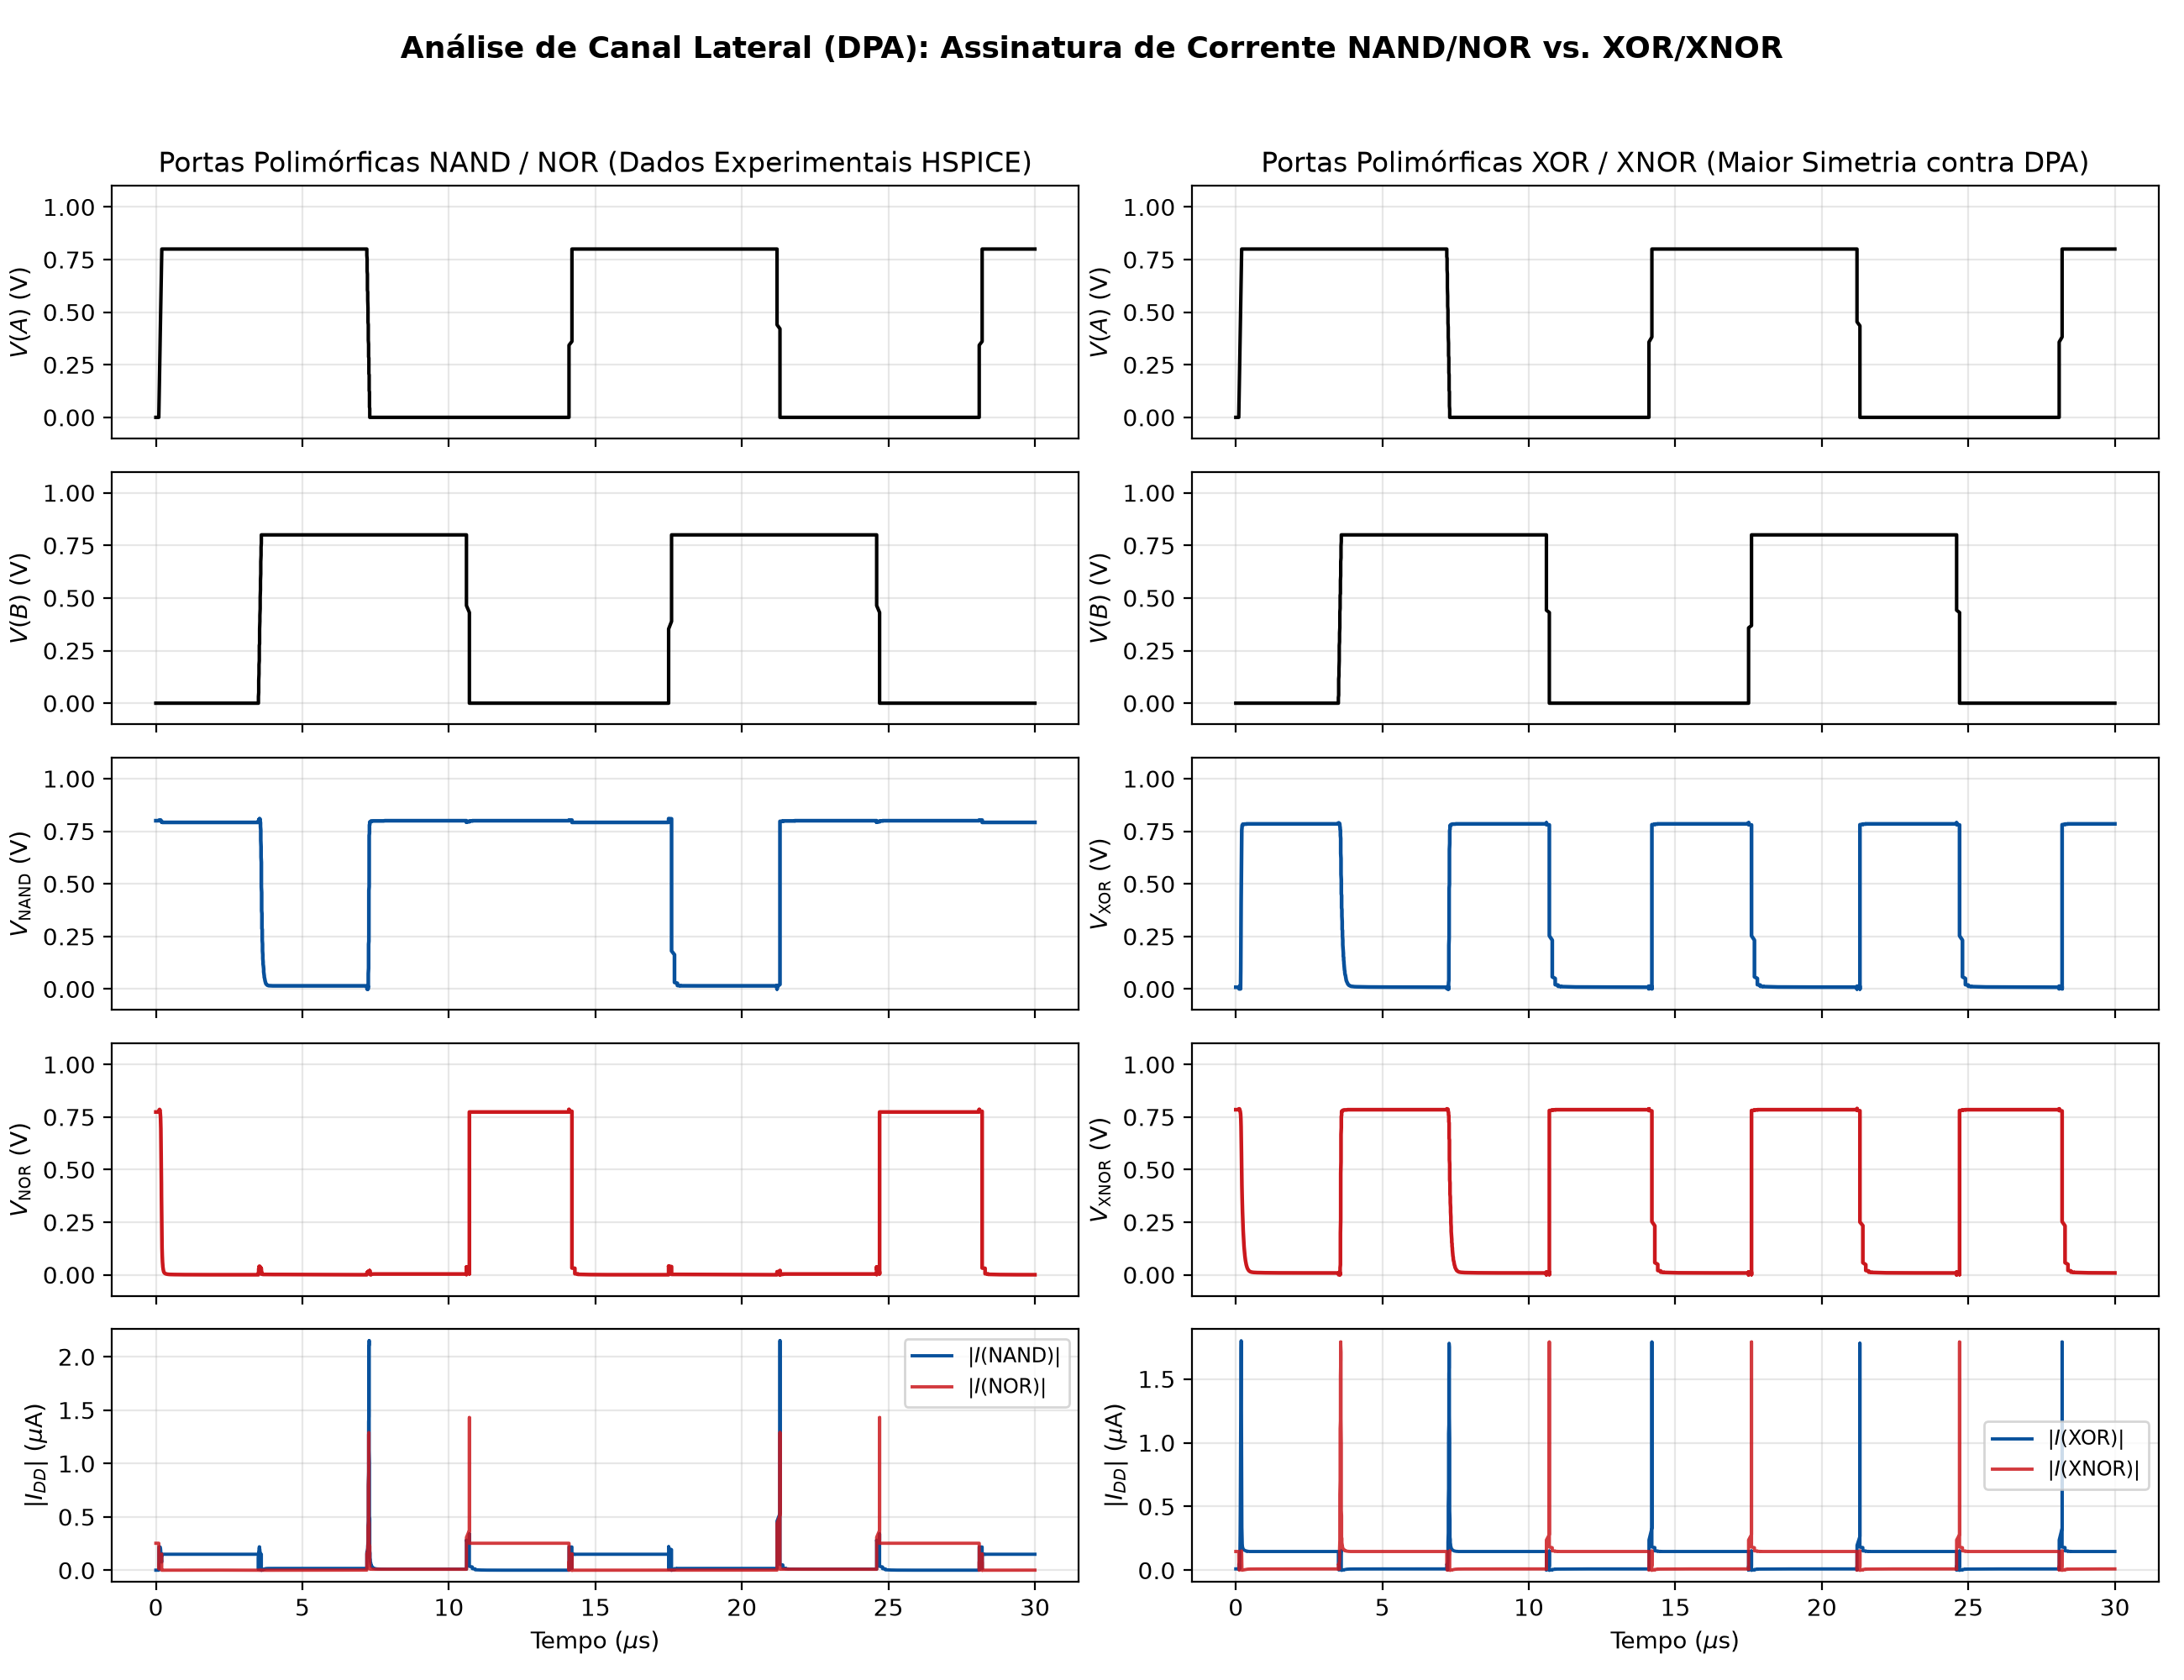
\includegraphics[width=0.92\textwidth]{m03_dpa_assinatura_corrente.png}
\caption{Comparativo de assinaturas de corrente $|I_{DD}|$ para ataque DPA entre \texttt{NAND}/\texttt{NOR} (esquerda) e \texttt{XOR}/\texttt{XNOR} (direita).}
\label{fig:m03_dpa}
\end{figure}

Nas 250 amostras de Monte Carlo (Figura~\ref{fig:m03_mc3d}), mesmo sob varia\c{c}\~{o}es severas nos trilhos ($V_{DD} \in [0{,}47;\ 1{,}15]\ \text{V}$), todas as quatro c\'{e}lulas atingiram $100{,}0\%$ de acerto l\'{o}gico sem sobreposi\c{c}\~{a}o entre os n\'{i}veis \texttt{'0'} e \texttt{'1'} em torno de $0{,}40\ \text{V}$. A valida\c{c}\~{a}o cruzada na grade $5 \times 5$ do \texttt{ngspice-47} (\texttt{ngspice\_supply\_sweep.csv}, Figura~\ref{fig:m03_hist_ret}) mostrou margem est\'{a}tica $(V_{00} - V_{11})$ entre $0{,}531\ \text{V}$ e $1{,}012\ \text{V}$ para $V_{DD} \ge 0{,}725\ \text{V}$ ou $V_{SS} \ge -0{,}05\ \text{V}$, degradando-se apenas no canto extremo ($V_{DD}=0{,}65\ \text{V},\ V_{SS}=-0{,}10\ \text{V}$), onde a margem cai para $0{,}153\ \text{V}$ ($V_{00} = 0{,}060\ \text{V}$ e $V_{11} = -0{,}093\ \text{V}$). Quanto \`{a} estabilidade temporal em n\'{o} flutuante (\texttt{bblc1}), ap\'{o}s os pulsos de excita\c{c}\~{a}o em $40$ e $80\ \mu\text{s}$, o potencial estabilizou em patamares distintos de $0{,}65\ \text{V}$ ($100\ \text{ns}$), $0{,}30\ \text{V}$ ($250\ \text{ns}$) e $0{,}20\ \text{V}$ ($500\ \text{ns}$) at\'{e} $111\ \mu\text{s}$.

\begin{figure}[htbp]
\centering
\begin{subfigure}{\textwidth}
  \centering
  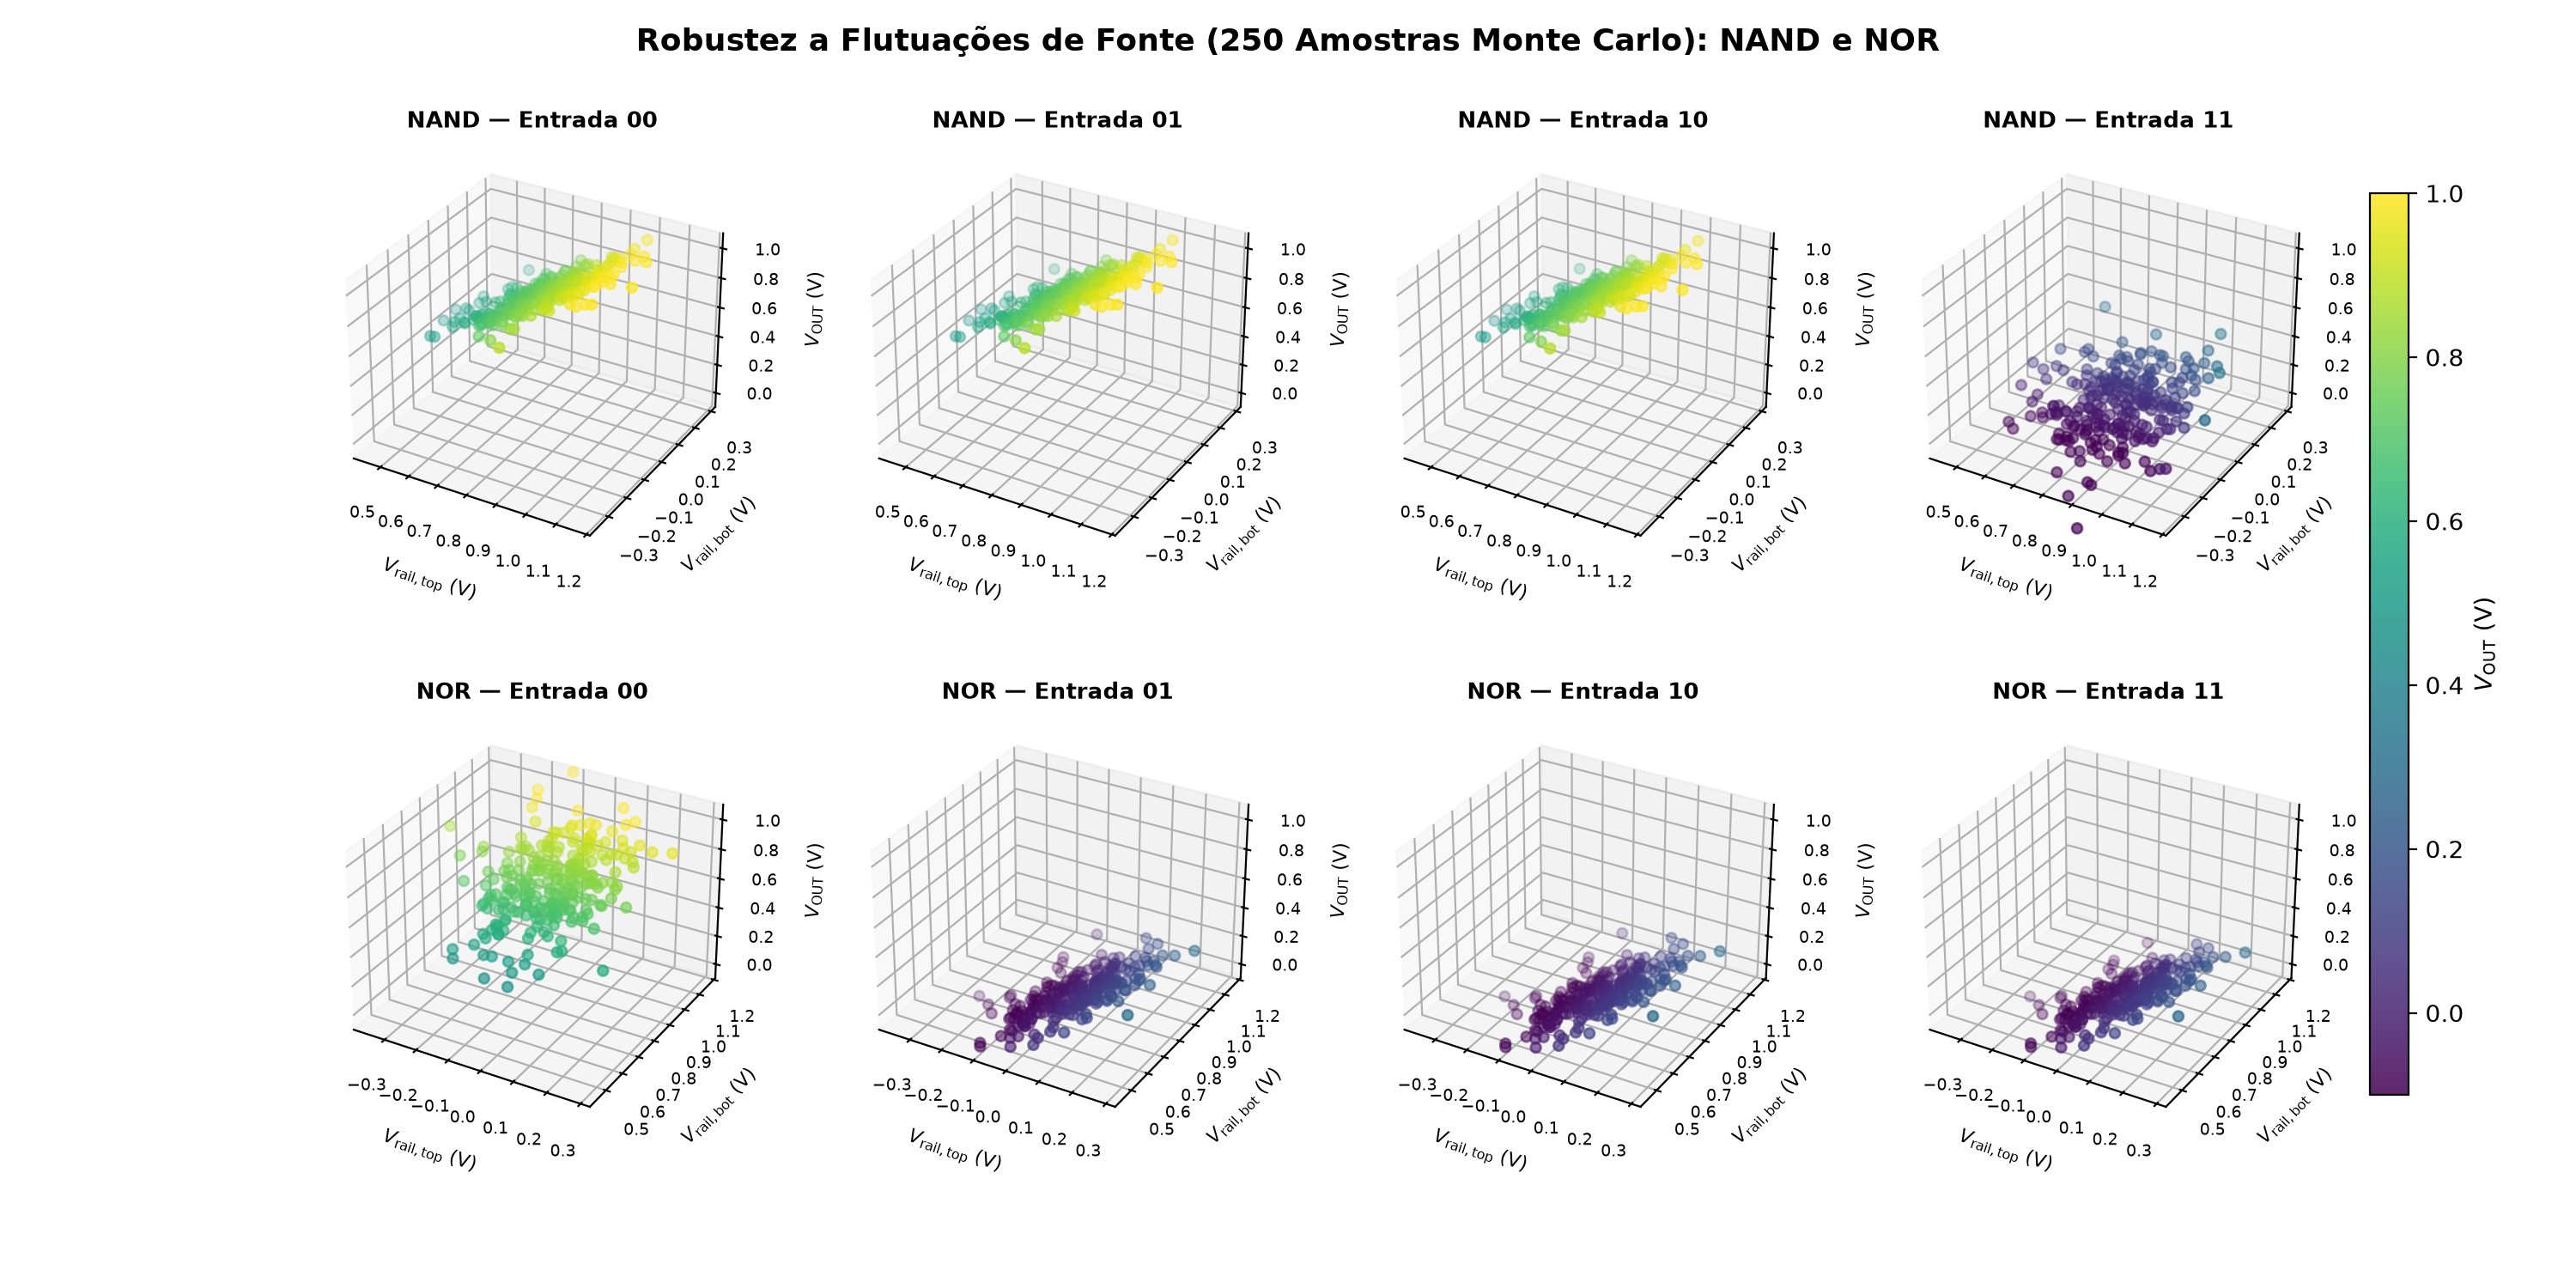
\includegraphics[width=0.95\textwidth]{m03_robustez_3d_nand_nor.png}
  \caption{Portas \texttt{NAND} e \texttt{NOR}.}
  \label{fig:m03_3d_nn}
\end{subfigure}
\par\medskip
\begin{subfigure}{\textwidth}
  \centering
  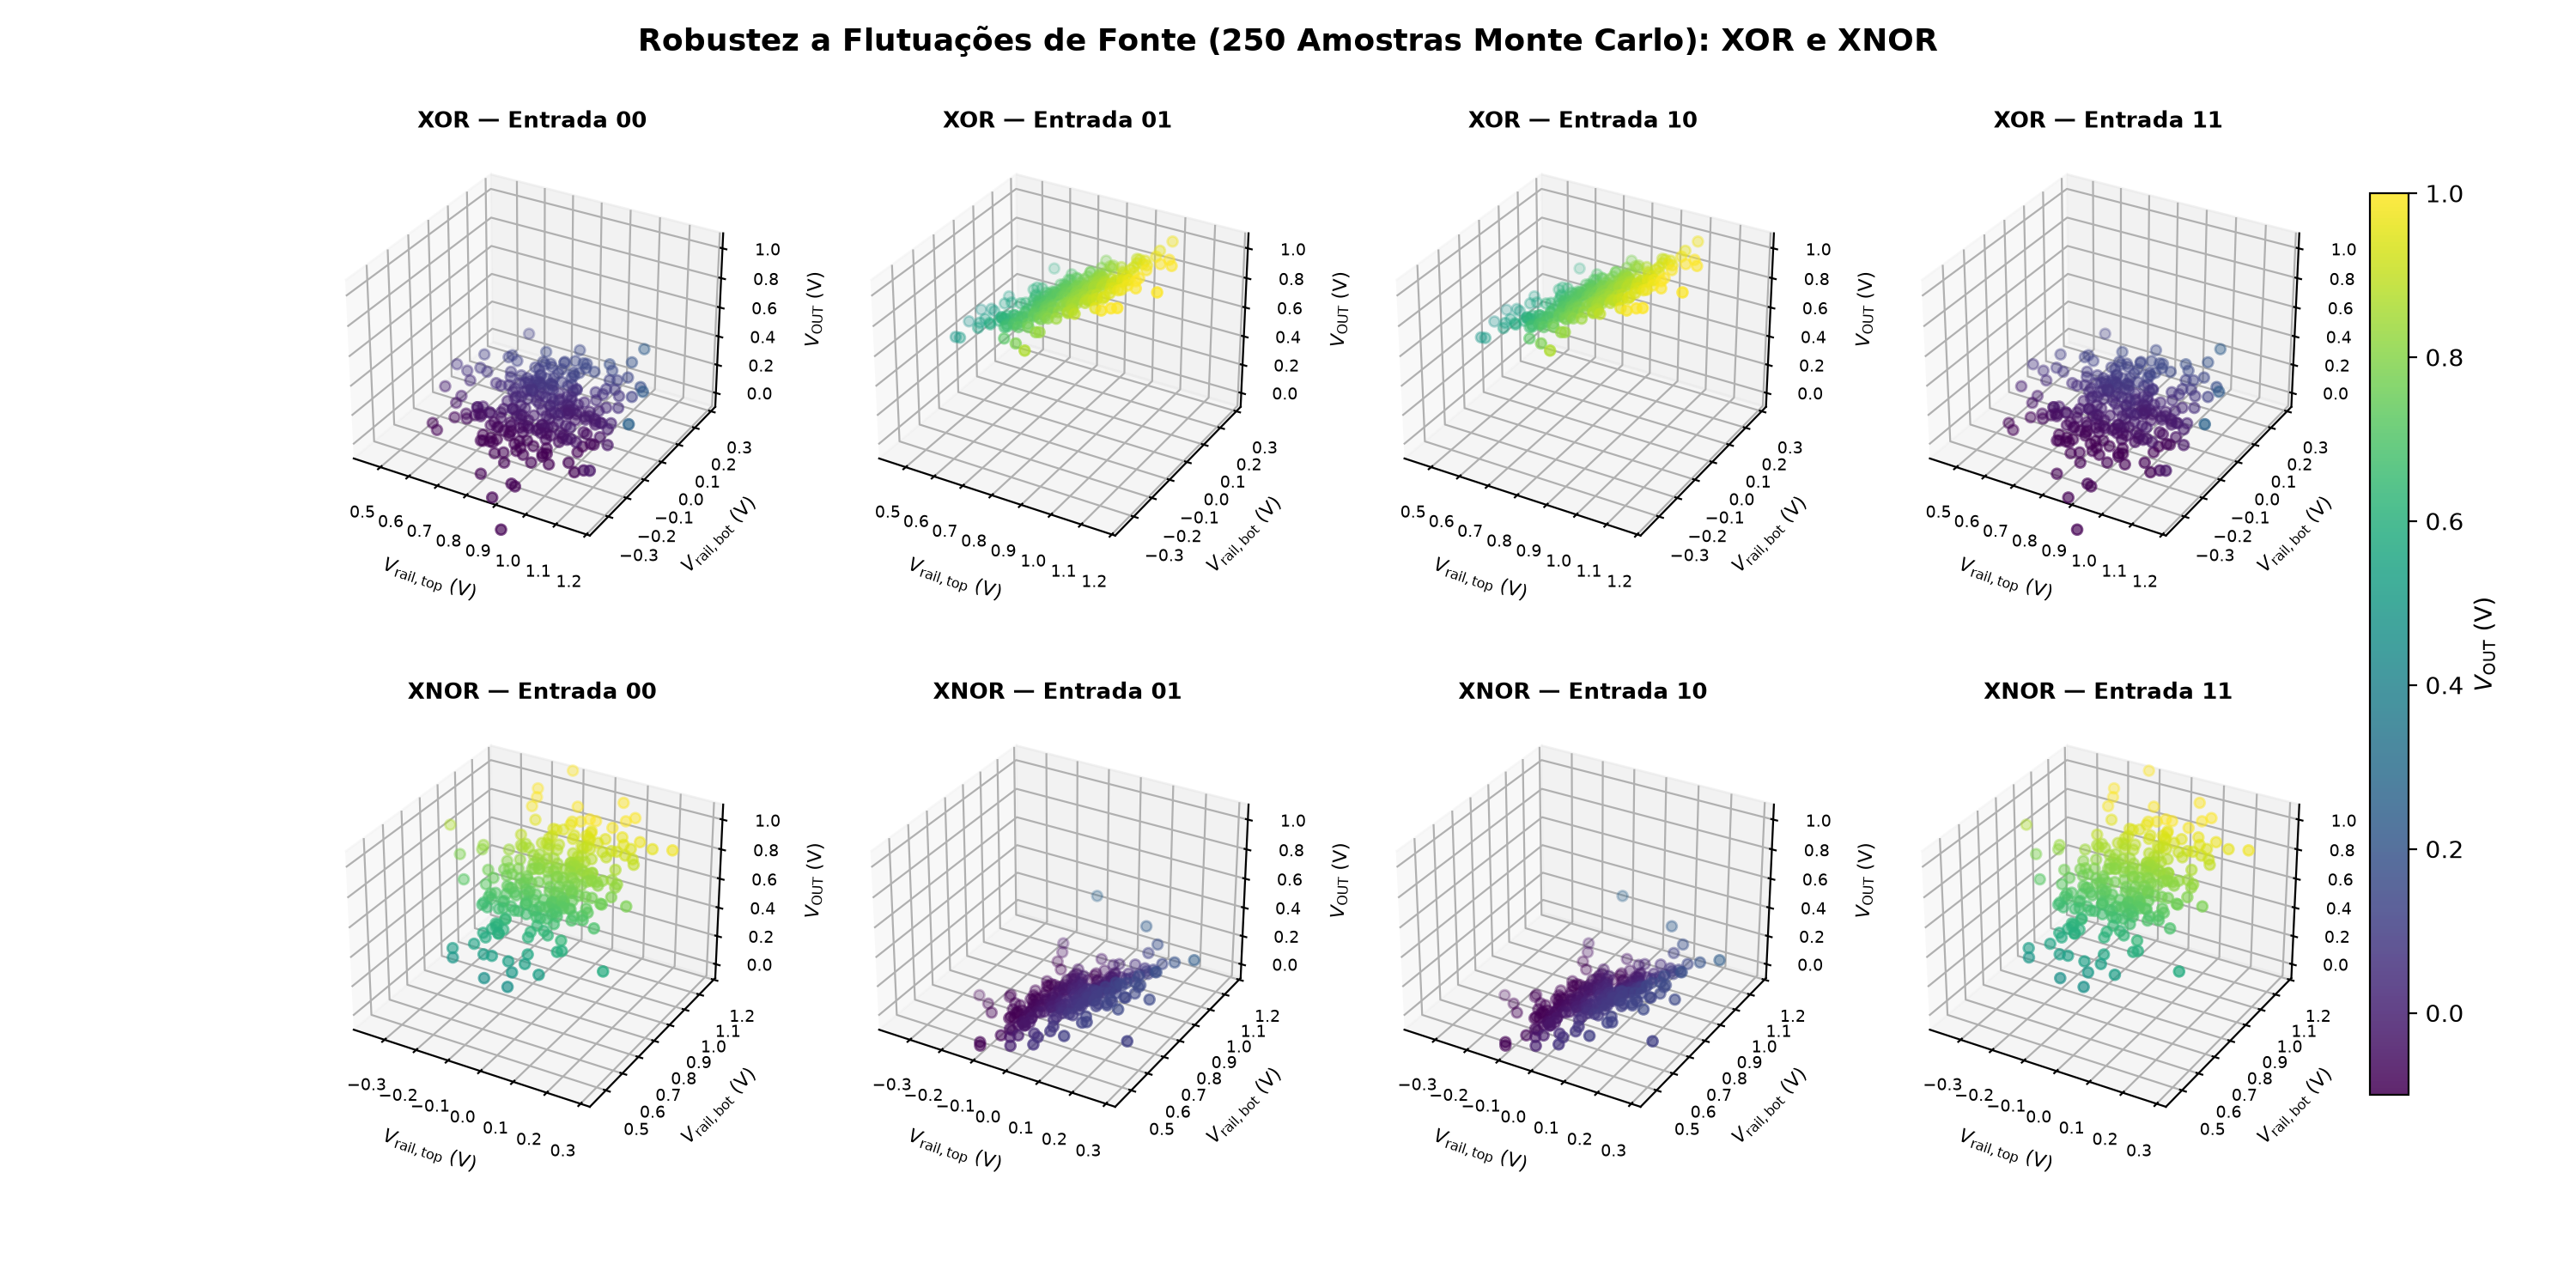
\includegraphics[width=0.95\textwidth]{m03_robustez_3d_xor_xnor.png}
  \caption{Portas \texttt{XOR} e \texttt{XNOR}.}
  \label{fig:m03_3d_xx}
\end{subfigure}
\caption{Superf\'{i}cies 3D de robustez ($V_{\mathrm{rail,top}} \times V_{\mathrm{rail,bot}} \times V_{\mathrm{OUT}}$) em 250 amostras Monte Carlo por vetor de entrada.}
\label{fig:m03_mc3d}
\end{figure}

\begin{figure}[htbp]
\centering
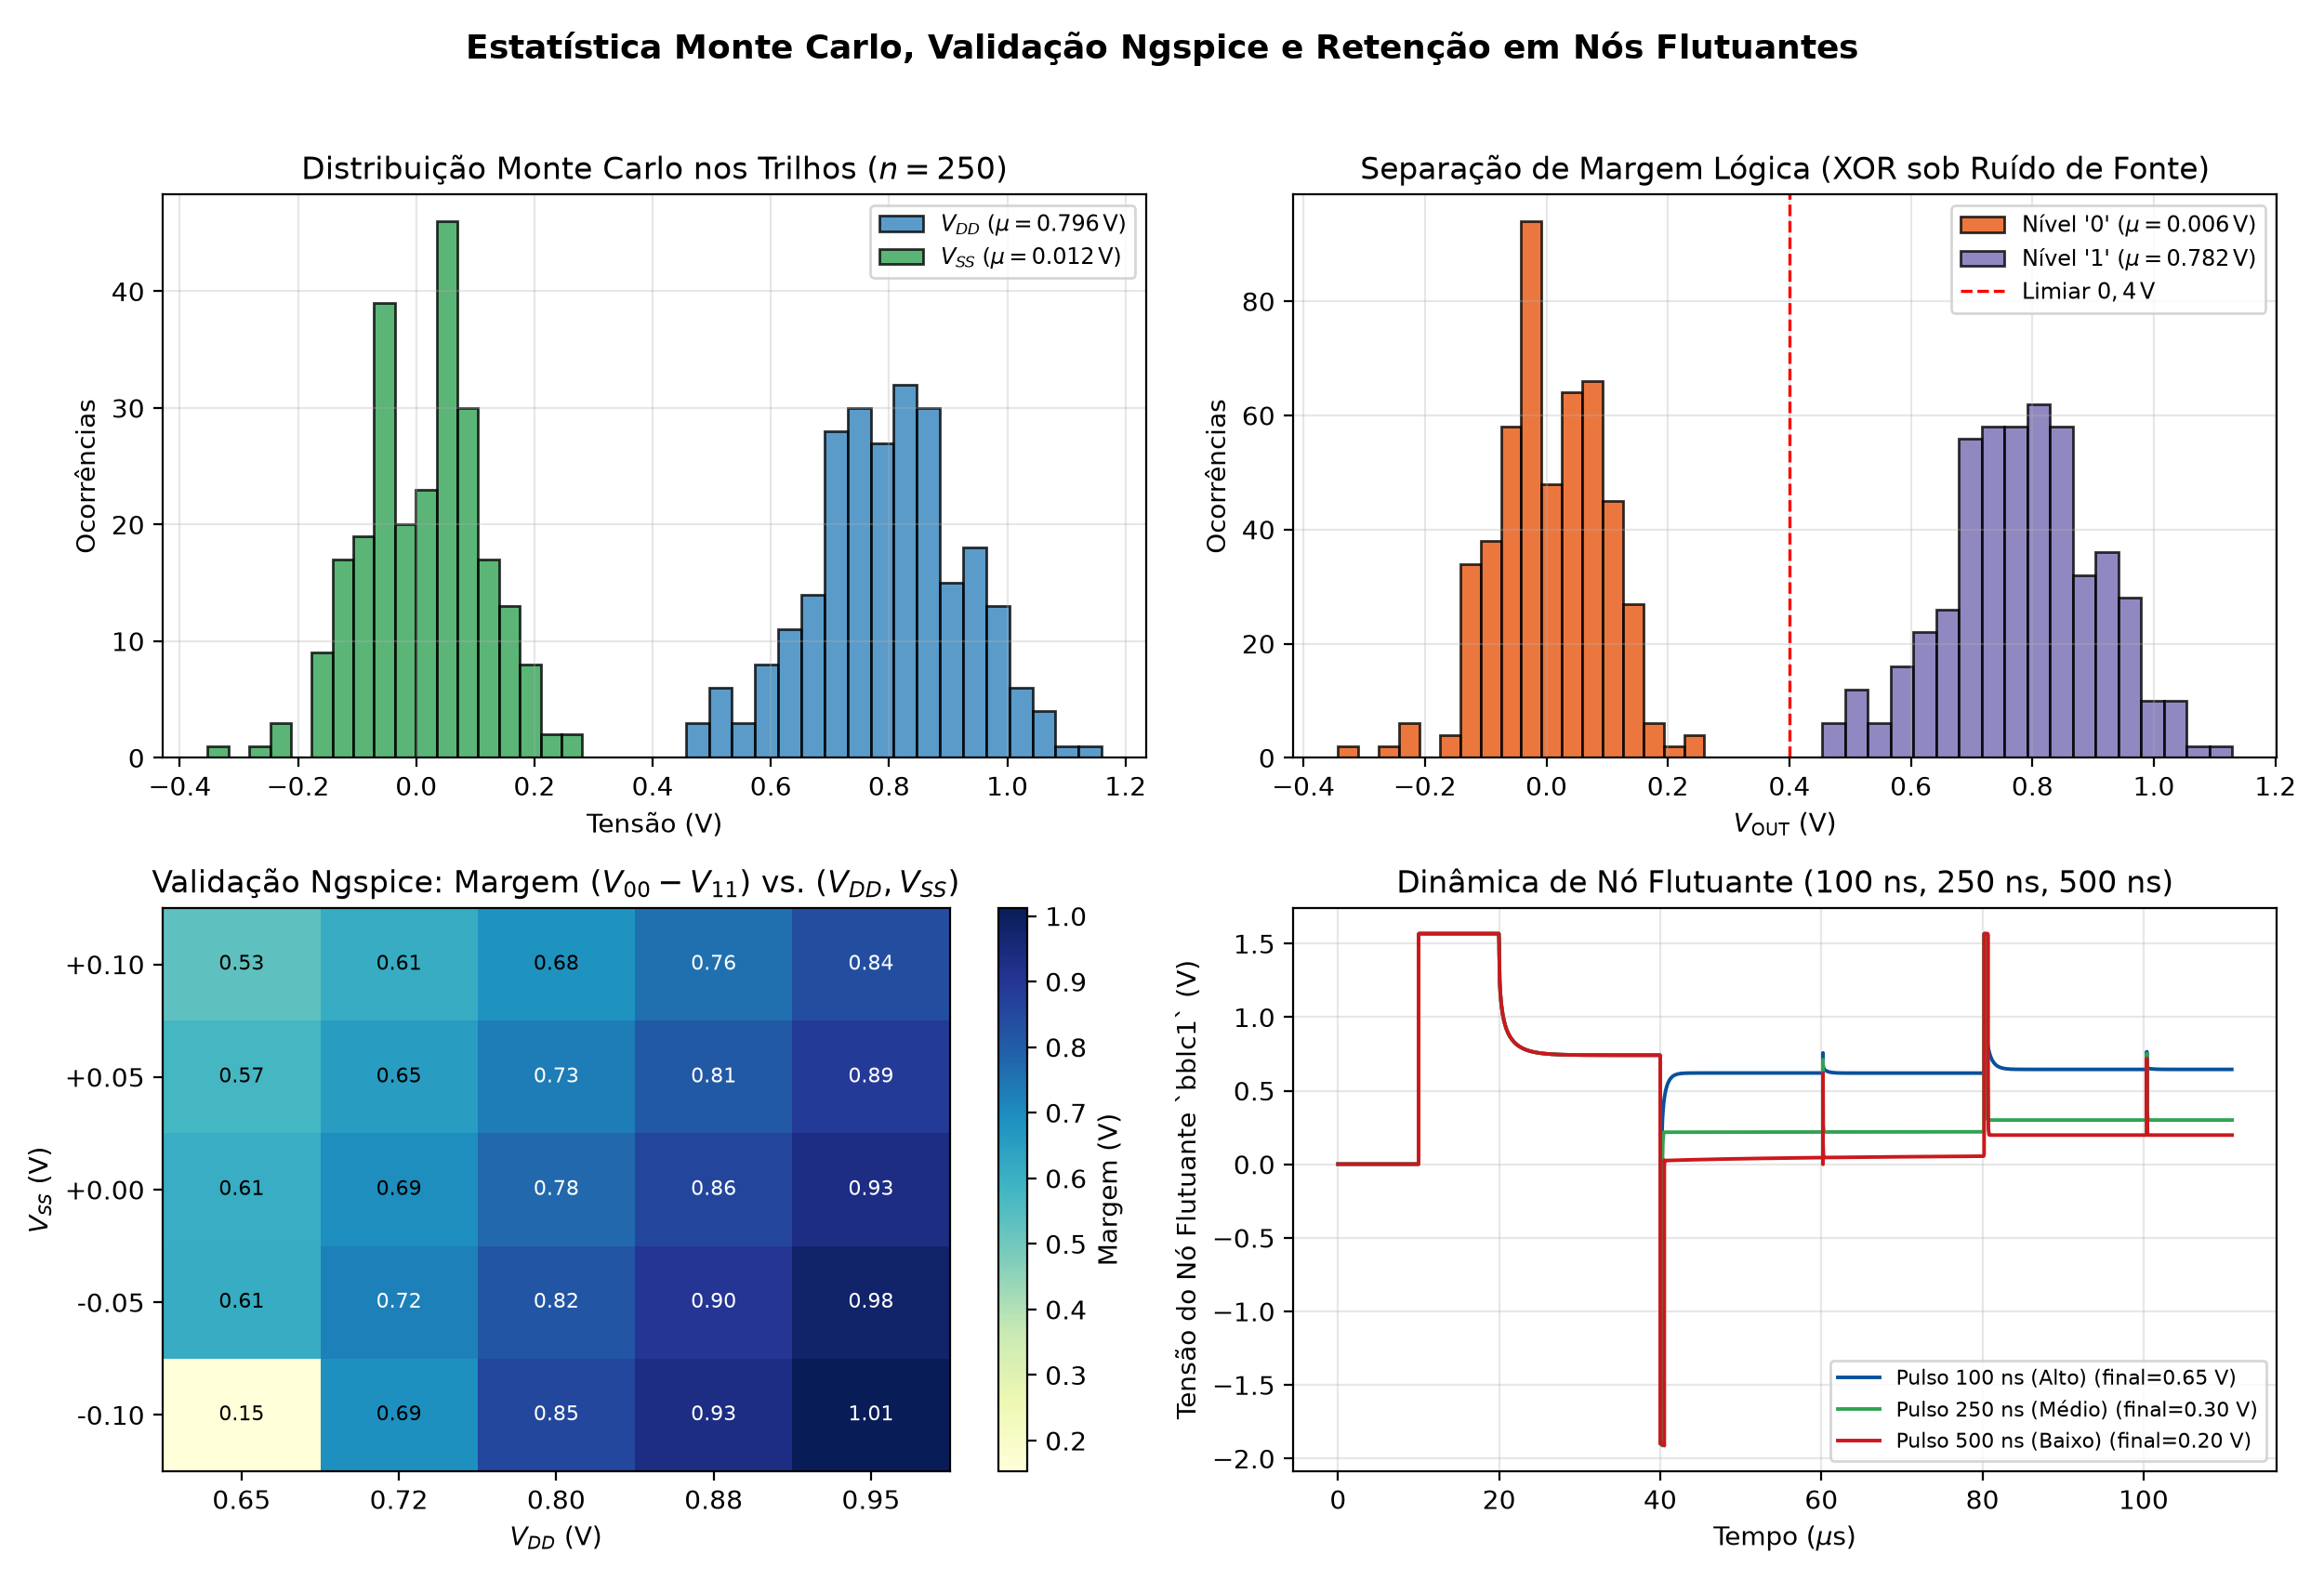
\includegraphics[width=0.92\textwidth]{m03_histogramas_e_retencao.png}
\caption{Distribui\c{c}\~{a}o Monte Carlo nos trilhos (superior esq.), separa\c{c}\~{a}o l\'{o}gica da \texttt{XOR} (superior dir.), mapa de margem $V_{DD}\times V_{SS}$ no \texttt{ngspice-47} (inferior esq.) e reten\c{c}\~{a}o em n\'{o} flutuante \texttt{bblc1} at\'{e} $111\ \mu\text{s}$ (inferior dir.).}
\label{fig:m03_hist_ret}
\end{figure}

\subsection{C\'{e}lula SRAM 6T com Bloqueio de Reten\c{c}\~{a}o (Mecanismo B)}\label{sec:res_sram}

A c\'{e}lula SRAM 6T satisfez todos os onze crit\'{e}rios de valida\c{c}\~{a}o transientes e est\'{a}ticos previstos para o Mecanismo B, conforme apresentado na Tabela~\ref{tab:sram_resultados}. Durante a simula\c{c}\~{a}o transiente de $30\ \text{ns}$ (Figura~\ref{fig:m04_tran}), sob $\text{Key} = 0$, a escrita do bit \texttt{'1'} ($0\text{--}6\ \text{ns}$) \'{e} retida ap\'{o}s o fechamento da \textit{Wordline} com $V(q) = 0{,}9768\ \text{V}$ e $V(qb) = 0{,}0020\ \text{V}$ em $t=12\ \text{ns}$ ($\Delta V_{\mathrm{Key0}} = 0{,}9747\ \text{V} > 0{,}80\ \text{V}$). No instante em que $\text{Key}$ comuta para $1$ ($t = 15\ \text{ns}$), mantendo $V_{DD} = 1{,}0\ \text{V}$ e $V_{SS} = 0{,}0\ \text{V}$ inalterados, a invers\~{a}o simult\^{a}nea das redes \textit{pull-up} (\textit{p-FET} $\to$ \textit{n-FET}) e \textit{pull-down} (\textit{n-FET} $\to$ \textit{p-FET}) provoca o colapso imediato do dado armazenado ($\Delta V_{\mathrm{Collapse1}} = 0{,}0841\ \text{V} < 0{,}15\ \text{V}$ em $18\ \text{ns}$). Na Fase 4 ($20\text{--}30\ \text{ns}$), mesmo for\c{c}ando o bit oposto durante o pulso de $\mathrm{WL}$, a c\'{e}lula volta a colapsar assim que $\mathrm{WL}$ fecha ($\Delta V_{\mathrm{Key1}} = 0{,}0762\ \text{V}$ em $28\ \text{ns}$).

\begin{table}[htbp]
\centering
\caption{M\'{e}tricas transientes ($30\ \text{ns}$) e margens est\'{a}ticas de ru\'{i}do (SNM) da c\'{e}lula SRAM 6T (\texttt{metricas\_sram\_6t.csv}).}
\label{tab:sram_resultados}
\footnotesize
\begin{tabular}{l c c c}
\toprule
\textbf{M\'{e}trica Extra\'{i}da} & \textbf{Valor Simulado} & \textbf{Crit\'{e}rio de Aceita\c{c}\~{a}o} & \textbf{Estado} \\
\midrule
$V(q)_{\mathrm{Hold}}$ ($\text{Key}=0,\ t=12\ \text{ns}$)   & $0{,}9768\ \text{V}$ & $> 0{,}80\ \text{V}$ & Aprovado \\
$V(qb)_{\mathrm{Hold}}$ ($\text{Key}=0,\ t=12\ \text{ns}$)  & $0{,}0020\ \text{V}$ & $< 0{,}20\ \text{V}$ & Aprovado \\
$\Delta V_{\mathrm{Key0}}$ ($t=12\ \text{ns}$)              & $0{,}9747\ \text{V}$ & $> 0{,}80\ \text{V}$ & Aprovado \\
$\Delta V_{\mathrm{Collapse1}}$ ($t=18\ \text{ns}$)         & $0{,}0841\ \text{V}$ & $< 0{,}15\ \text{V}$ & Aprovado \\
$\Delta V_{\mathrm{Key1}}$ ($t=28\ \text{ns}$)              & $0{,}0762\ \text{V}$ & $< 0{,}15\ \text{V}$ & Aprovado \\
$\mathrm{SNM}_{\mathrm{Hold}}$ ($\text{Key}=0,\ \mathrm{WL}=0\ \text{V}$)           & $167{,}12\ \text{mV}$ & $> 150\ \text{mV}$ & Aprovado \\
$\mathrm{SNM}_{\mathrm{Read,Unassisted}}$ ($\text{Key}=0,\ \mathrm{WL}=1{,}0\ \text{V}$) & $0{,}00\ \text{mV}$ & $0\ \text{mV}$ (\textit{Read Disturb}) & Diagnosticado \\
$\mathrm{SNM}_{\mathrm{Read,Assist}}$ ($\text{Key}=0,\ \mathrm{WL}=0{,}30\ \text{V}$) & $66{,}23\ \text{mV}$ & $> 50\ \text{mV}$ & Aprovado \\
$\mathrm{SNM}_{\mathrm{Hold}}$ ($\text{Key}=1,\ \mathrm{WL}=0\ \text{V}$)           & $0{,}00\ \text{mV}$ & $= 0\ \text{mV}$ & Aprovado \\
$\mathrm{SNM}_{\mathrm{Read,Assist}}$ ($\text{Key}=1,\ \mathrm{WL}=0{,}30\ \text{V}$) & $0{,}00\ \text{mV}$ & $= 0\ \text{mV}$ & Aprovado \\
$\mathrm{SNM}_{\mathrm{Read,Unassisted}}$ ($\text{Key}=1,\ \mathrm{WL}=1{,}0\ \text{V}$) & $0{,}00\ \text{mV}$ & $= 0\ \text{mV}$ & Aprovado \\
\bottomrule
\end{tabular}
\end{table}

\begin{figure}[htbp]
\centering
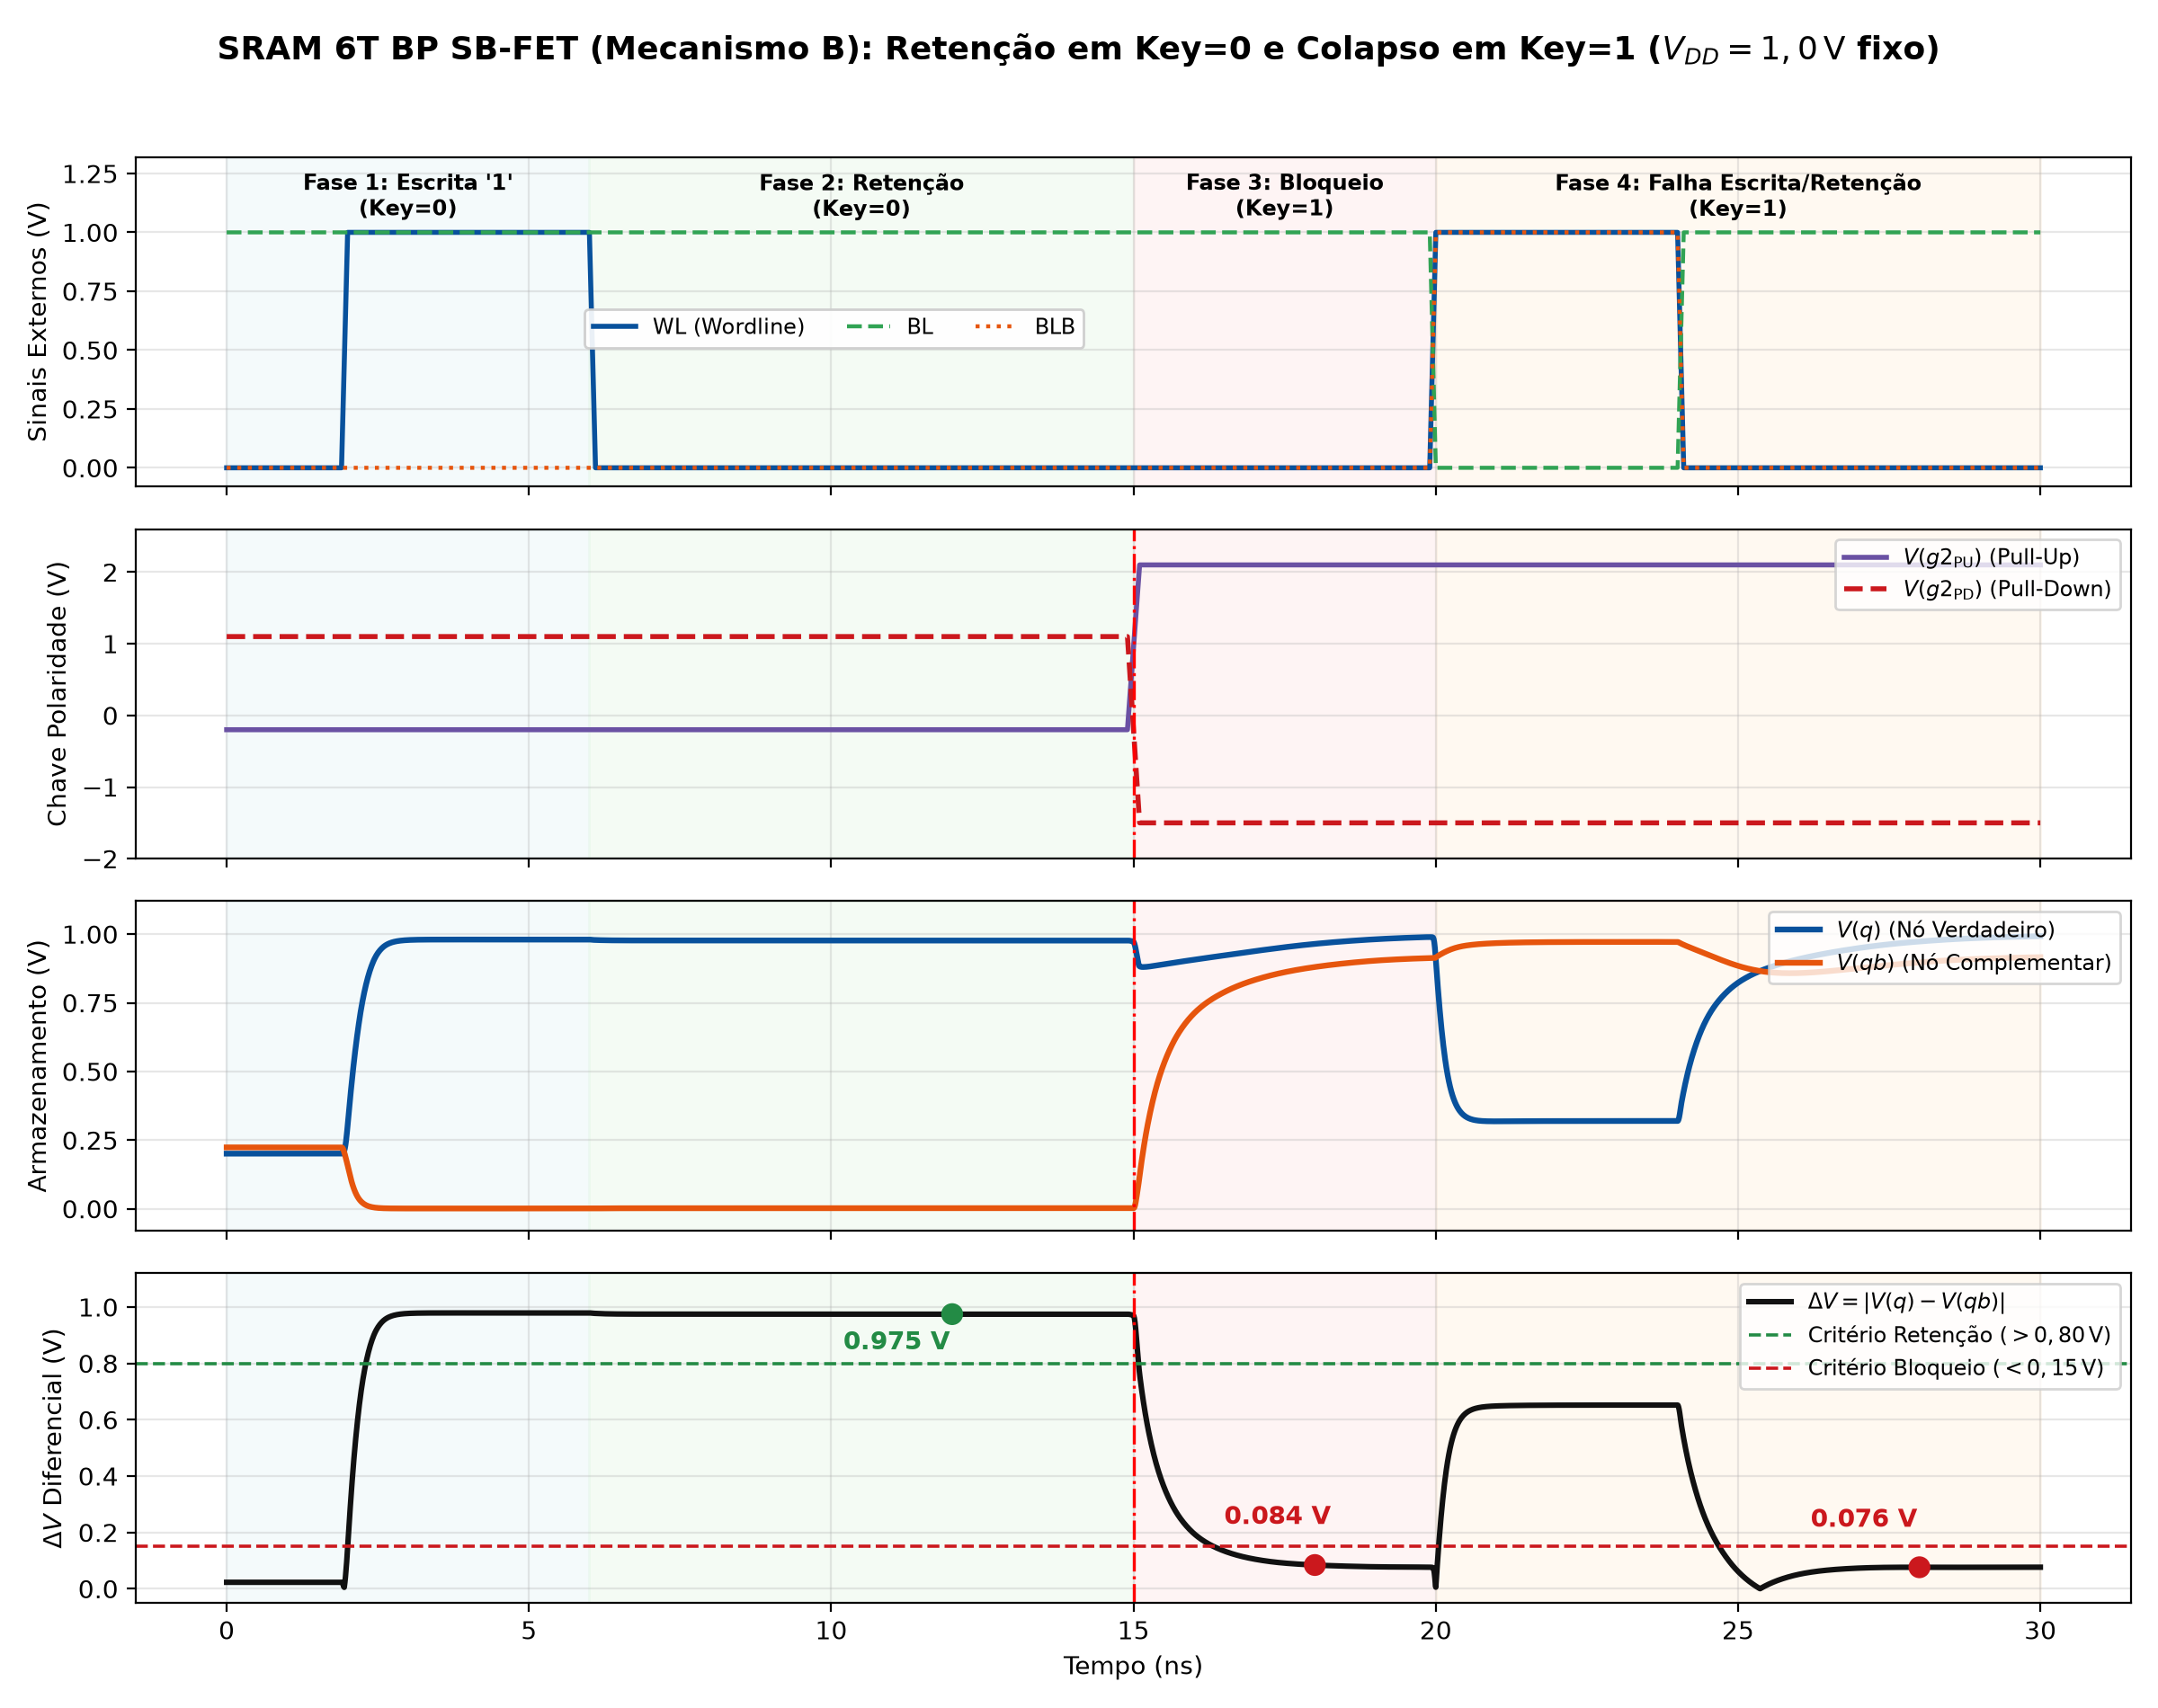
\includegraphics[width=0.92\textwidth]{m04_sram_transiente_30ns.png}
\caption{Simula\c{c}\~{a}o transiente de $30\ \text{ns}$ da SRAM 6T em quatro fases: escrita e reten\c{c}\~{a}o segura sob $\text{Key}=0$ ($0\text{--}15\ \text{ns}$) seguidas de auto-destrui\c{c}\~{a}o do bit e falha de reescrita sob $\text{Key}=1$ ($15\text{--}30\ \text{ns}$).}
\label{fig:m04_tran}
\end{figure}

\begin{figure}[htbp]
\centering
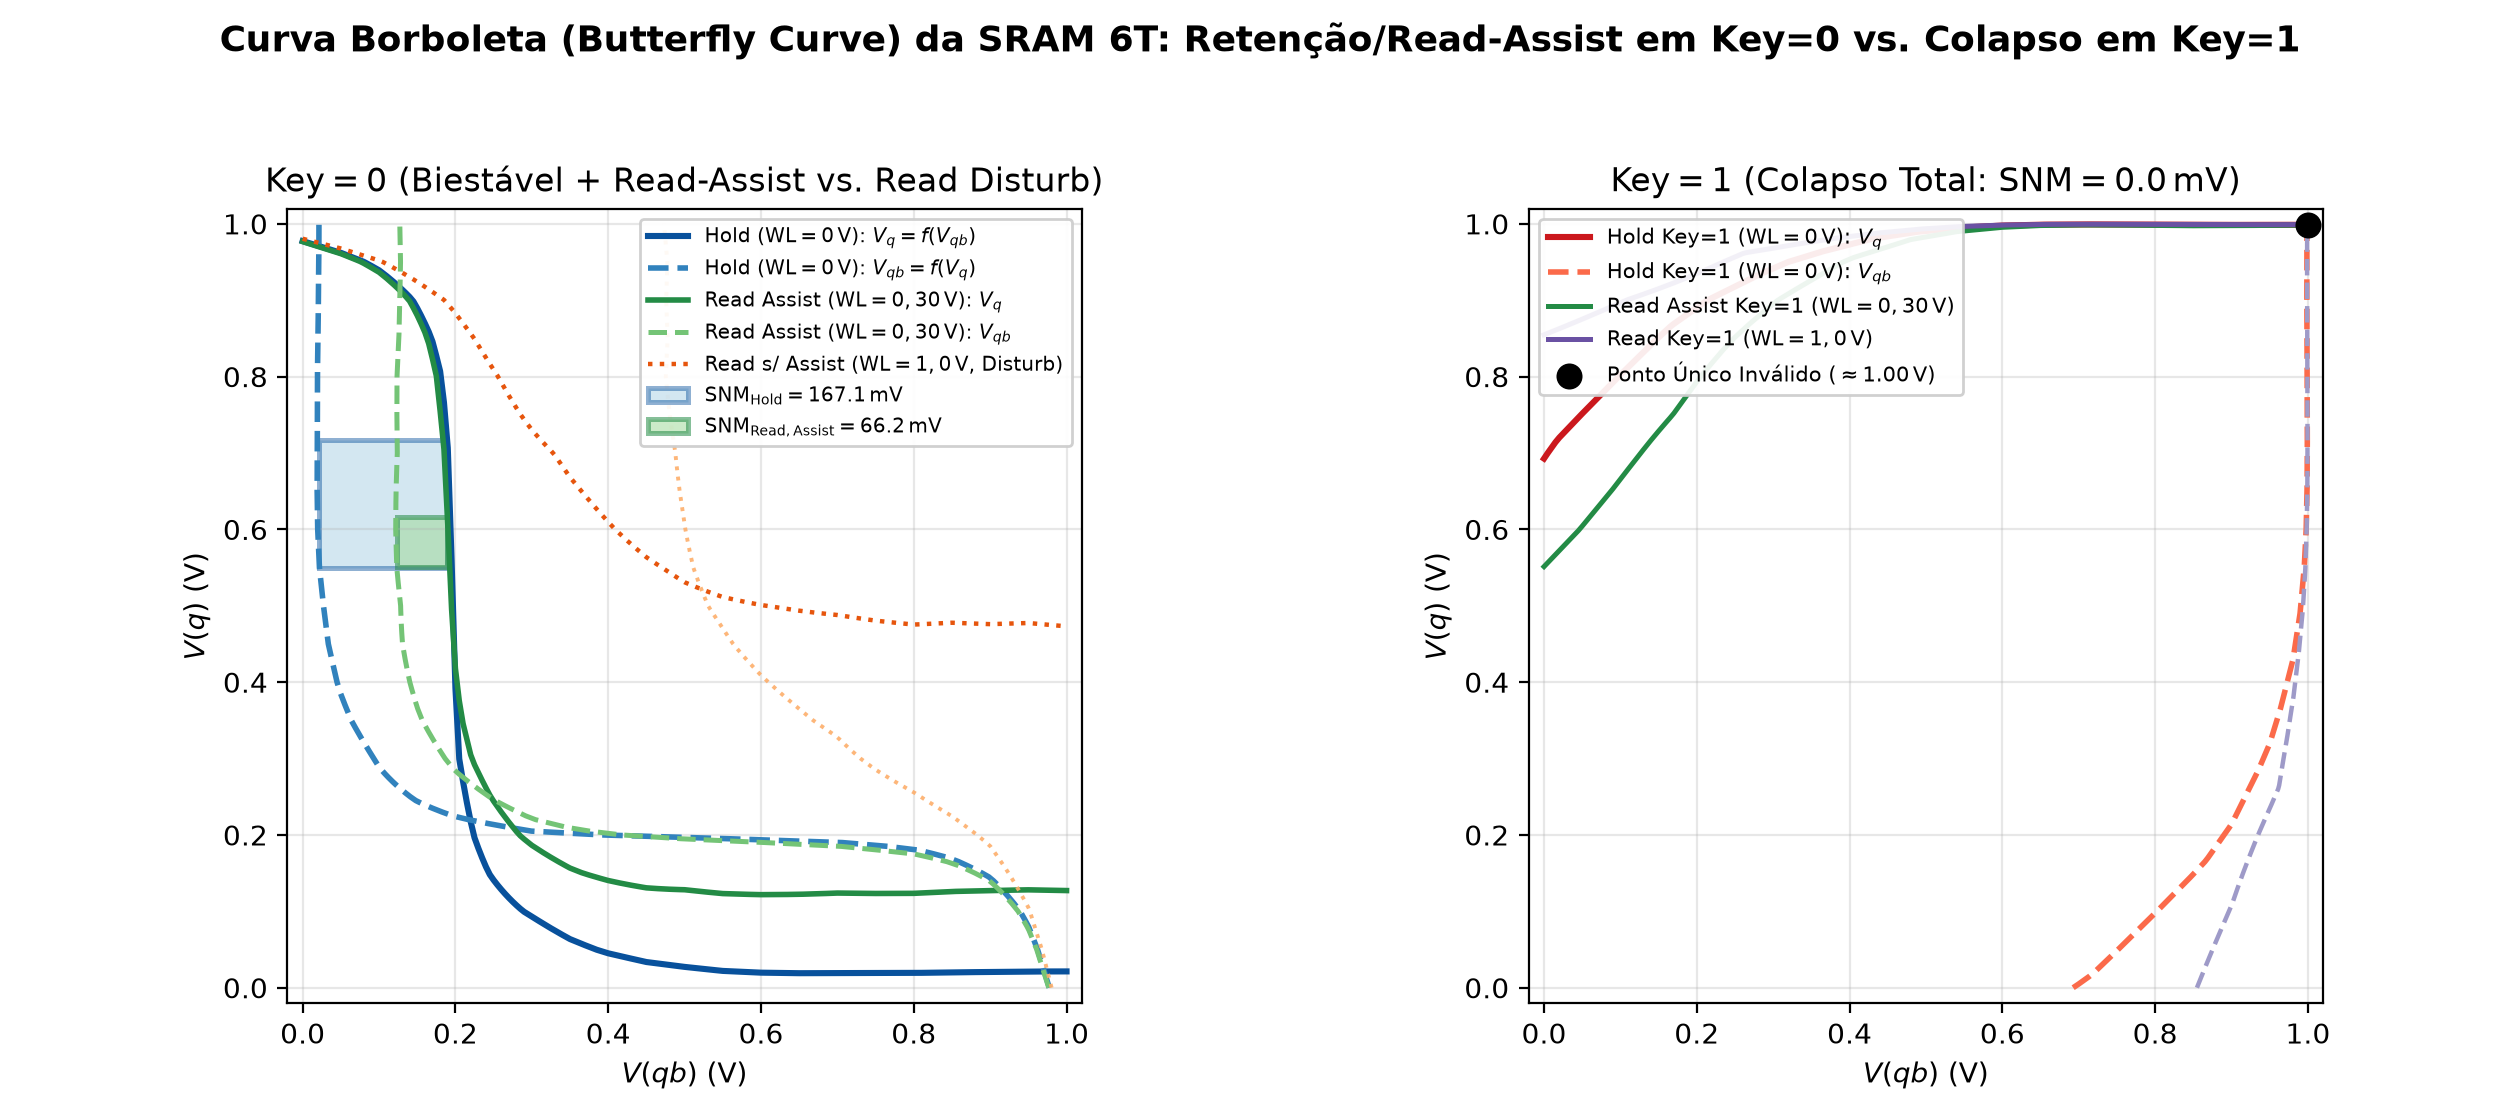
\includegraphics[width=0.92\textwidth]{m04_sram_curva_borboleta_snm.png}
\caption{Curvas borboleta e quadrados m\'{a}ximos inscritos de SNM da SRAM 6T para $\text{Key}=0$ (Hold, Read-Assist e Read sem assist\^{e}ncia com \textit{Read Disturb}) e $\text{Key}=1$ (colapso total para linha monost\'{a}vel).}
\label{fig:m04_snm}
\end{figure}

Dois achados f\'{i}sicos relevantes emergiram da an\'{a}lise das curvas borboleta (Figura~\ref{fig:m04_snm}). Primeiramente, verificou-se com o modelo 4D \texttt{v2} que a polariza\c{c}\~{a}o inicialmente proposta em $V_{g2,\mathrm{PU}} = -0{,}5\ \text{V}$ ($V_{g2,s} = -1{,}5\ \text{V}$) reduz a corrente \textit{p-FET} de $1{,}79$ para $0{,}37\ \mu\text{A}$ (em $V_{gp}=-1{,}0\ \text{V}$) por deslocamento de $V_{fb}$, rebaixando $\mathrm{SNM}_{\mathrm{Hold}}$ para $49{,}4\ \text{mV}$; o ajuste de sintonia para $V_{g2,\mathrm{PU}} = -0{,}2\ \text{V}$ ($V_{g2,s} = -1{,}2\ \text{V}$) restaurou integralmente a simetria sem alterar as larguras $W$, atingindo $\mathrm{SNM}_{\mathrm{Hold}} = 167{,}12\ \text{mV}$. Em segundo lugar, diagnosticou-se o fen\^{o}meno de \textit{Read Disturb} na leitura sem assist\^{e}ncia ($\mathrm{WL}=1{,}0\ \text{V}$, $\mathrm{SNM}=0{,}00\ \text{mV}$), o qual foi mitigado por \textit{Wordline Underdrive Read-Assist} em $\mathrm{WL}=0{,}30\ \text{V}$, recuperando $\mathrm{SNM}_{\mathrm{Read,Assist}} = 66{,}23\ \text{mV}$ enquanto todas as condi\c{c}\~{o}es sob $\text{Key}=1$ mantiveram $\mathrm{SNM}=0{,}00\ \text{mV}$.

\subsection{Somador Completo Polim\'{o}rfico Criptogr\'{a}fico (28 Transistores)}\label{sec:res_fa}

No Somador Completo polim\'{o}rfico de 28 transistores (M\'{o}dulo \texttt{05}), a chave autorizada $K_1 K_0 = 00$ produziu exatid\~{a}o de $100{,}00\%$ nos oito mintermos ($000 \to 111$, Figura~\ref{fig:m05_wave}), sustentando excurs\~{a}o superior a $94\%$ na sa\'{i}da \texttt{Sum} (dom\'{i}nio $1{,}5\ \text{V}$: \texttt{'0'} $\le 0{,}0012\ \text{V}$, \texttt{'1'} $\ge 1{,}4129\ \text{V}$) e superior a $92\%$ na sa\'{i}da \texttt{Cout} (dom\'{i}nio $0{,}8\ \text{V}$: \texttt{'0'} $\le 0{,}0124\ \text{V}$, \texttt{'1'} $\ge 0{,}7526\ \text{V}$) ap\'{o}s tr\^{e}s est\'{a}gios l\'{o}gicos cascateados.

\begin{table}[htbp]
\centering
\caption{Corrup\c{c}\~{a}o funcional e Dist\^{a}ncia de Hamming (HD) por chave criptogr\'{a}fica $(K_1, K_0)$ no Full Adder 28T.}
\label{tab:fa_hamming}
\resizebox{\textwidth}{!}{%
\begin{tabular}{c l c c c c c c}
\toprule
\textbf{Chave} $K_1K_0$ & \textbf{Configura\c{c}\~{a}o} (\texttt{XXOR1} + \texttt{Cout}) & \textbf{Erros} \texttt{Sum} & \textbf{HD} \texttt{Sum} & \textbf{Erros} \texttt{Cout} & \textbf{HD} \texttt{Cout} & \textbf{HD Total} (/16) & \textbf{Acur\'{a}cia} \\
\midrule
\texttt{00} (Correta) & \texttt{XOR} + \texttt{NAND}  & $0/8$ & $0{,}0\%$   & $0/8$ & $0{,}0\%$  & $0\ (0{,}00\%)$   & $100{,}00\%$ \\
\texttt{01} (Errada)  & \texttt{XNOR} + \texttt{NAND} & $8/8$ & $100{,}0\%$ & $3/8$ & $37{,}5\%$ & $11\ (68{,}75\%)$ & $31{,}25\%$  \\
\texttt{10} (Errada)  & \texttt{XOR} + \texttt{NOR}   & $0/8$ & $0{,}0\%$   & $3/8$ & $37{,}5\%$ & $3\ (18{,}75\%)$  & $81{,}25\%$  \\
\texttt{11} (Errada)  & \texttt{XNOR} + \texttt{NOR}  & $8/8$ & $100{,}0\%$ & $0/8$ & $0{,}0\%$  & $8\ (50{,}00\%)$  & $50{,}00\%$  \\
\bottomrule
\end{tabular}}
\end{table}

Conforme a Tabela~\ref{tab:fa_hamming} e a Figura~\ref{fig:m05_hd}, todas as chaves incorretas corrompem a opera\c{c}\~{a}o aritm\'{e}tica sem necessidade de transistores adicionais dedicados a bloqueio. Em $K_1K_0 = 01$, a invers\~{a}o do n\'{o} $P \to \overline{P}$ propaga-se tanto para \texttt{Sum} ($100{,}0\%$) quanto para \texttt{Cout} ($37{,}5\%$), resultando em $\mathrm{HD}_{\mathrm{Total}} = 68{,}75\%$. Em $K_1K_0 = 11$, manifesta-se uma propriedade alg\'{e}brica de dualidade de De Morgan: ao converter simultaneamente \texttt{XXOR1} em \texttt{XNOR} ($\overline{P}$) e \texttt{XG1}--\texttt{XG3} em \texttt{NOR}, obt\'{e}m-se $\overline{\overline{A+B} + \overline{\overline{P}+C_{\mathrm{in}}}} = (A+B)\cdot(\overline{P}+C_{\mathrm{in}}) = A\cdot B + C_{\mathrm{in}}\cdot(A\oplus B)$, restaurando integralmente \texttt{Cout} enquanto \texttt{Sum} permanece $100{,}0\%$ invertida ($\mathrm{HD}_{\mathrm{Total}} = 50{,}00\%$).

\begin{figure}[htbp]
\centering
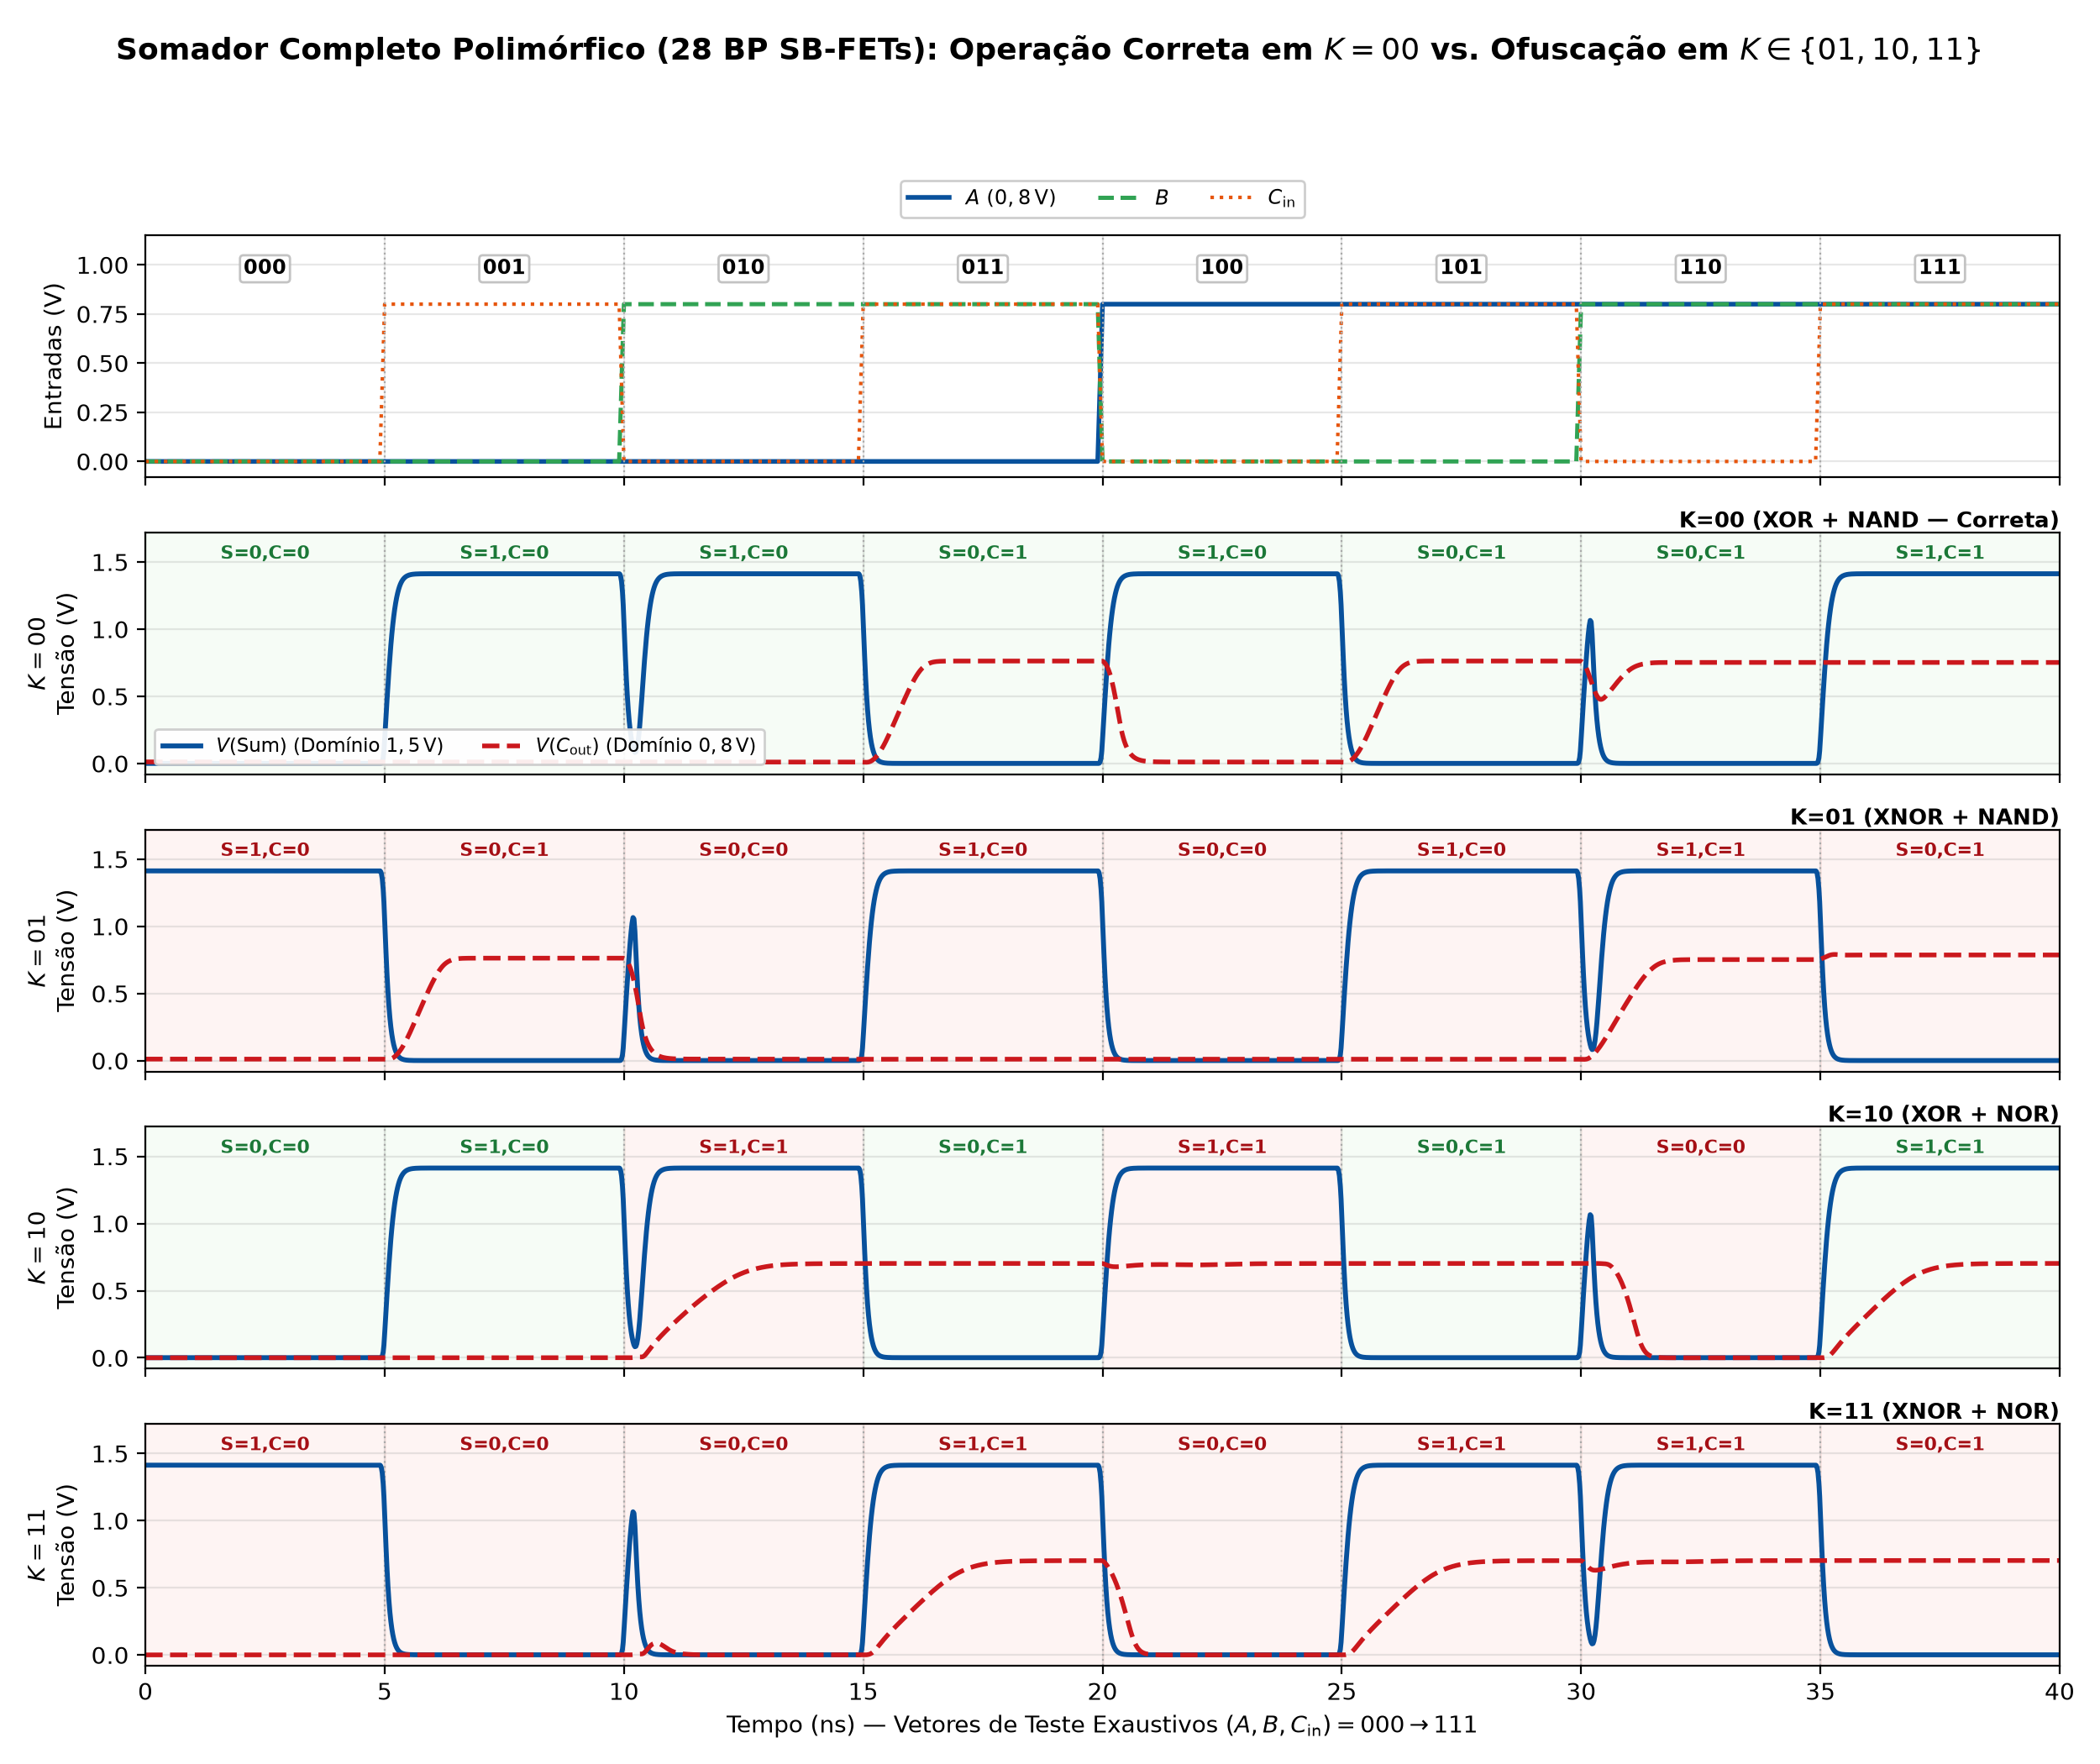
\includegraphics[width=0.92\textwidth]{m05_full_adder_waveforms.png}
\caption{Formas de onda transientes ($40\ \text{ns}$, mintermos \texttt{000} a \texttt{111}) do Somador Completo polim\'{o}rfico de 28 transistores nas quatro chaves $K_1K_0$.}
\label{fig:m05_wave}
\end{figure}

\begin{figure}[htbp]
\centering
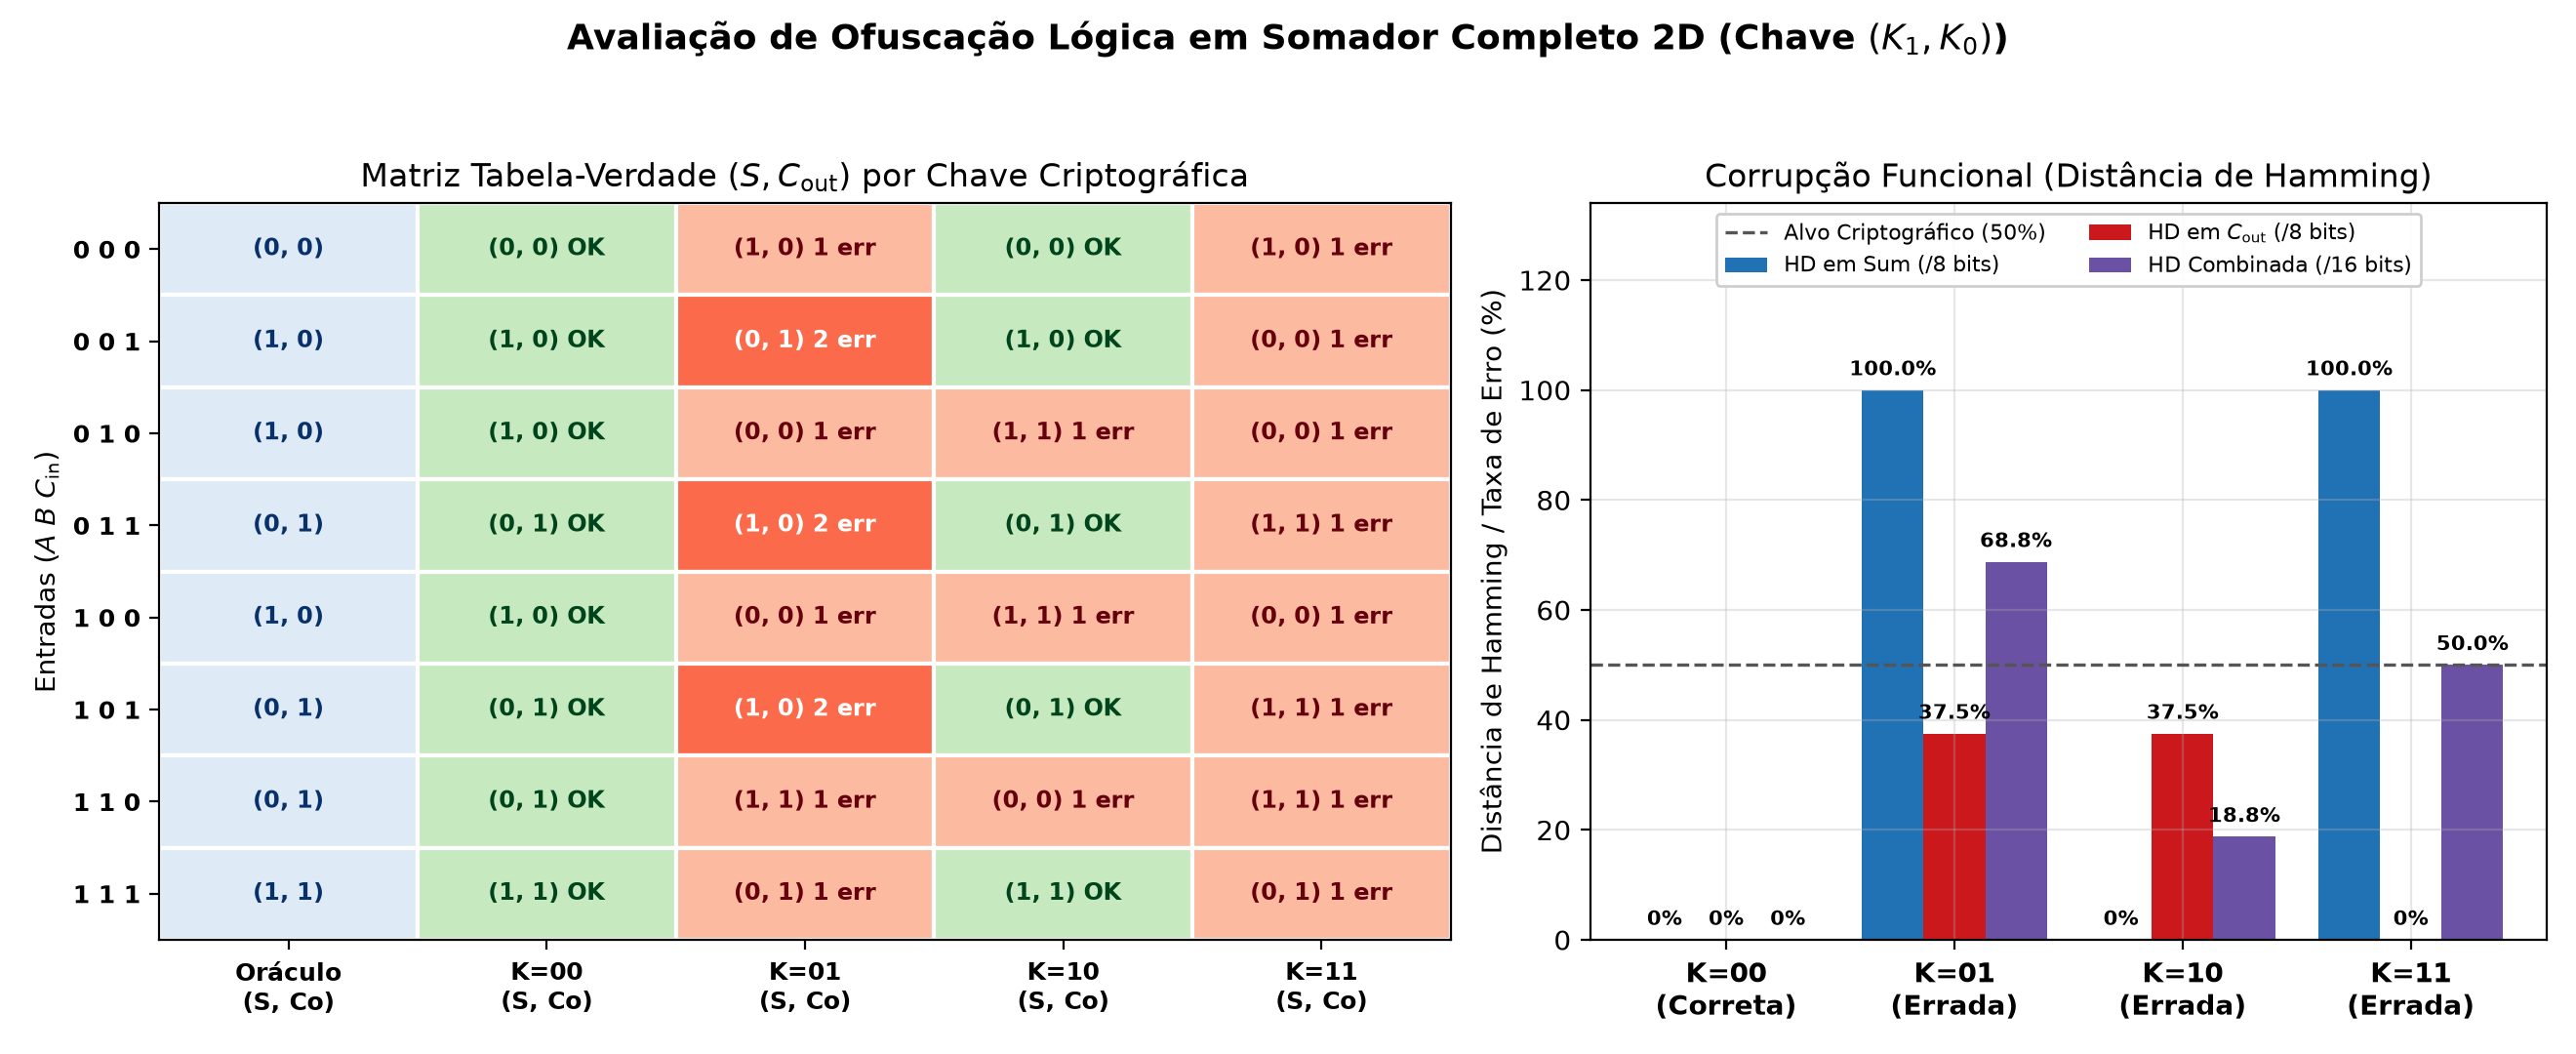
\includegraphics[width=0.92\textwidth]{m05_matriz_tabelas_verdade_hamming.png}
\caption{Matriz de tabelas-verdade e Dist\^{a}ncia de Hamming (HD) do Somador Completo polim\'{o}rfico para as chaves \texttt{00}, \texttt{01}, \texttt{10} e \texttt{11}.}
\label{fig:m05_hd}
\end{figure}

\subsection{Fronteira Operacional sob Tens\~{o}es N\~{a}o Padronizadas}\label{sec:res_fronteira}

A varredura dos 292 pontos dentro do dom\'{i}nio experimentalmente medido das tabelas LUT (M\'{o}dulo \texttt{06}) demonstrou que o deslocamento das tens\~{o}es de alimenta\c{c}\~{a}o, entrada e polaridade pode conduzir aos tr\^{e}s regimes previstos: manuten\c{c}\~{a}o da fun\c{c}\~{a}o nominal (\texttt{CORRETA}), transmuta\c{c}\~{a}o para outra fun\c{c}\~{a}o booleana digital (\texttt{OUTRA\_FUNCAO}) ou colapso em estados anal\'{o}gicos indefinidos (\texttt{INDEFINIDO\_ANALOGICO}), conforme sumarizado na Tabela~\ref{tab:fronteira_resumo}.

\begin{table}[htbp]
\centering
\caption{Distribui\c{c}\~{a}o dos 292 pontos simulados sob tens\~{o}es n\~{a}o padronizadas no dom\'{i}nio das LUTs.}
\label{tab:fronteira_resumo}
\resizebox{\textwidth}{!}{%
\begin{tabular}{l c c c c l}
\toprule
\textbf{Subexperimento} & \textbf{Pontos} & \texttt{CORRETA} & \texttt{OUTRA\_FUNCAO} & \texttt{INDEFINIDO} & \textbf{Fun\c{c}\~{o}es Equivalentes Observadas} \\
\midrule
\texttt{NAND}/\texttt{NOR} ($V_{DD}\times$ Pol.) & $70$  & $29$ & $35$ & $6$  & \texttt{NAND} ($13$), \texttt{NOR} ($17$), \texttt{CONST\_0} ($34$), \texttt{X} ($6$) \\
\texttt{NAND}/\texttt{NOR} ($V_{g2,n}\times V_{g2,p}$) & $72$  & $60$ & $0$  & $12$ & \texttt{NAND} ($27$), \texttt{NOR} ($33$), \texttt{X} ($12$) \\
\texttt{XOR}/\texttt{XNOR} ($V_{DD}\times V_{\mathrm{in}}$) & $100$ & $44$ & $46$ & $10$ & \texttt{XOR} ($22$), \texttt{XNOR} ($22$), \texttt{CONST\_0} ($38$), \texttt{CONST\_1} ($8$), \texttt{X} ($10$) \\
\texttt{XOR}/\texttt{XNOR} ($V_{g,\mathrm{top}}=0\ \text{V}$) & $50$  & $44$ & $6$  & $0$  & \texttt{XOR} ($22$), \texttt{XNOR} ($22$), \texttt{CONST\_1} ($6$) \\
\bottomrule
\end{tabular}}
\end{table}

Na fam\'{i}lia \texttt{NAND}/\texttt{NOR} (Figuras~\ref{fig:m06_nn_vdd} e \ref{fig:m06_nn_asym}), observou-se um evento cr\'{i}tico de \textbf{convers\~{a}o espont\^{a}nea \texttt{NAND} $\to$ \texttt{NOR} sem altera\c{c}\~{a}o da chave}: em $V_{DD} = 0{,}65\ \text{V}$ sob sub-polariza\c{c}\~{a}o moderada ($+0{,}4/-1{,}1\ \text{V}$), a porta configurada como \texttt{NAND} ($\text{Key}=0$) produziu o padr\~{a}o l\'{o}gico \texttt{[1000]} ($V_{00}=0{,}5412\ \text{V}$, $V_{01}=0{,}1073\ \text{V}$, $V_{10}=0{,}1410\ \text{V}$, $V_{11}=0{,}0206\ \text{V}$), id\^{e}ntico \`{a} tabela-verdade da sua fun\c{c}\~{a}o dual \texttt{NOR}. Fisicamente, nos vetores \texttt{01} e \texttt{10}, apenas um \textit{p-FET} enfraquecido tenta elevar a sa\'{i}da enquanto a rede s\'{e}rie \textit{n-FET} em $+0{,}4\ \text{V}$ sustenta fuga suficiente para descarregar o n\'{o}, vencendo o \textit{pull-up} somente quando os dois \textit{p-FETs} conduzem em paralelo (\texttt{00}). Para $V_{DD} \le 0{,}50\ \text{V}$, $34$ dos $70$ pontos degeneraram em \texttt{CONST\_0} (\texttt{0000}). Na grade de assimetria em $V_{DD}=0{,}80\ \text{V}$, $60$ de $72$ pontos operaram corretamente e $12$ entraram em regime anal\'{o}gico indefinido (\texttt{[1X10]}, \texttt{[10X0]}, \texttt{[111X]}, \texttt{[X000]}), com destaque para a faixa n\~{a}o monot\^{o}nica em $V(g2,s)_p = -1{,}50\ \text{V}$ na \texttt{NAND} (em raz\~{a}o do deslocamento $\Delta V_{fb} \approx -0{,}25\ \text{V}$, $V_{01}$ colapsou para $0{,}163\text{--}0{,}496\ \text{V}$ em quatro das seis colunas \textit{n-FET}), ao passo que $V(g2,s)_p \in \{-1{,}35;\ -1{,}20\}\ \text{V}$ obteve $100\%$ de acerto.

Na fam\'{i}lia \texttt{XOR}/\texttt{XNOR} (Figura~\ref{fig:m06_xor_mapa}), avaliaram-se $150$ pontos ($88$ corretos, $52$ classificados como \texttt{OUTRA\_\allowbreak FUNCAO} e $10$ em estado indefinido \texttt{INDEFINIDO\_\allowbreak ANALOGICO}), revelando travamentos sim\'{e}tricos opostos: para $V_{DD} \in [0{,}60;\ 0{,}80]\ \text{V}$, $38$ casos degeneraram para \texttt{CONST\_0} (\texttt{0000}) por \textit{overdrive} insuficiente do ramo \textit{p-FET}; inversamente, com $V_{DD}$ elevado ($1{,}20\text{--}1{,}50\ \text{V}$) e $V_{\mathrm{in}}$ baixo ($0{,}40\text{--}0{,}60\ \text{V}$), $14$ casos travaram em \texttt{CONST\_1} (\texttt{1111}, $V_{\mathrm{out}} \ge 1{,}4154\ \text{V}$ a $1{,}50\ \text{V}$) acompanhados de elevada corrente est\'{a}tica ($0{,}536\text{--}1{,}222\ \mu\text{A}$). Na fronteira intermedi\'{a}ria ($V_{DD} = 1{,}00\ \text{V}$), a polariza\c{c}\~{a}o nominal ($+0{,}8/-1{,}5\ \text{V}$) entrou em regime indefinido para $V_{\mathrm{in}} \ge 0{,}80\ \text{V}$, enquanto a sub-polariza\c{c}\~{a}o ($+0{,}2/-0{,}9\ \text{V}$) restaurou a opera\c{c}\~{a}o correta com margem normalizada entre $86{,}4\%$ e $88{,}4\%$.

\begin{figure}[htbp]
\centering
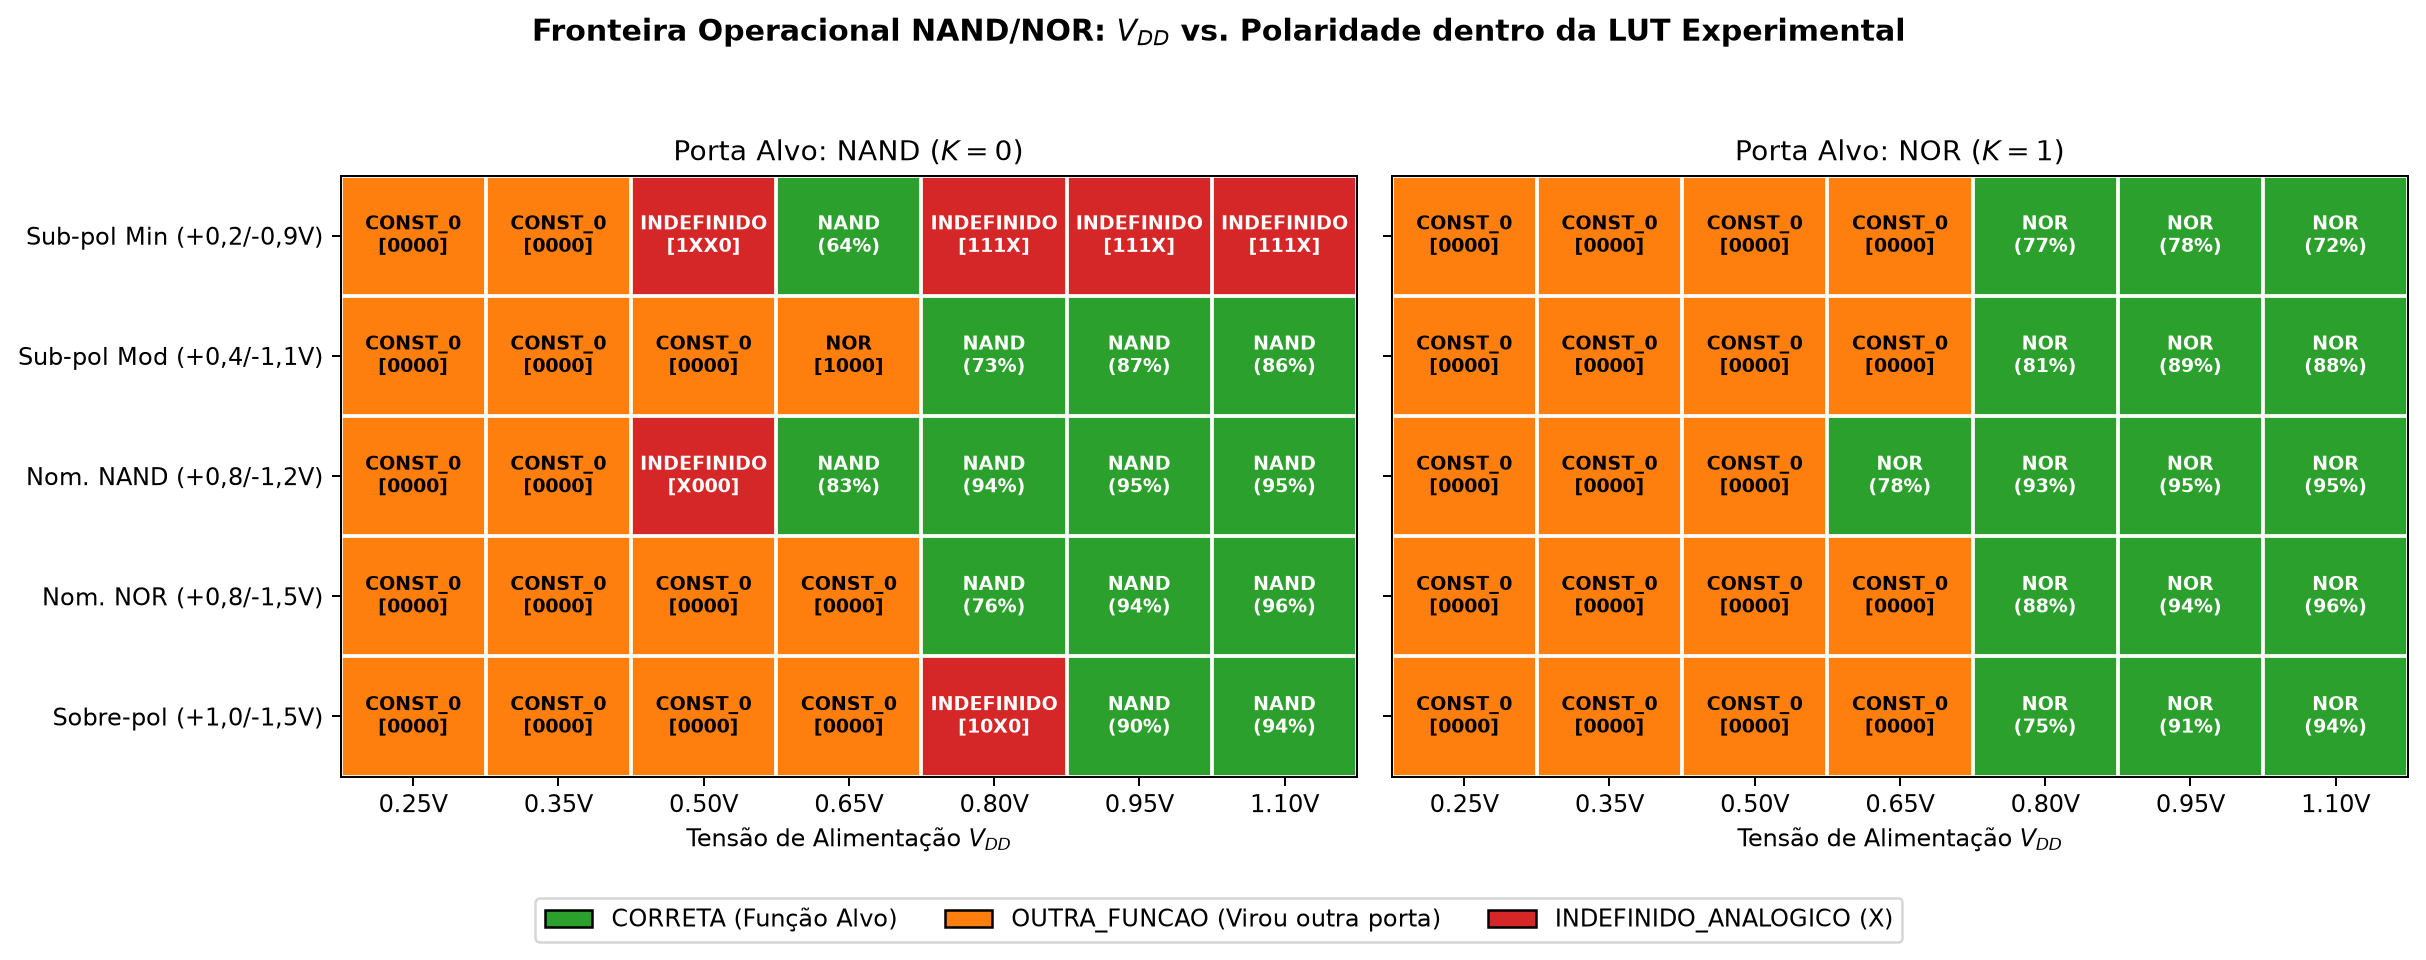
\includegraphics[width=0.92\textwidth]{m06_nand_nor_mapa_vdd_polaridade.png}
\caption{Mapa de fases operacionais ($V_{DD} \times$ polaridade) da porta \texttt{NAND}/\texttt{NOR}, destacando a convers\~{a}o espont\^{a}nea \texttt{NAND} $\to$ \texttt{NOR} em $V_{DD}=0{,}65\ \text{V}$ e o colapso \texttt{CONST\_0} em sub-tens\~{a}o.}
\label{fig:m06_nn_vdd}
\end{figure}

\begin{figure}[htbp]
\centering
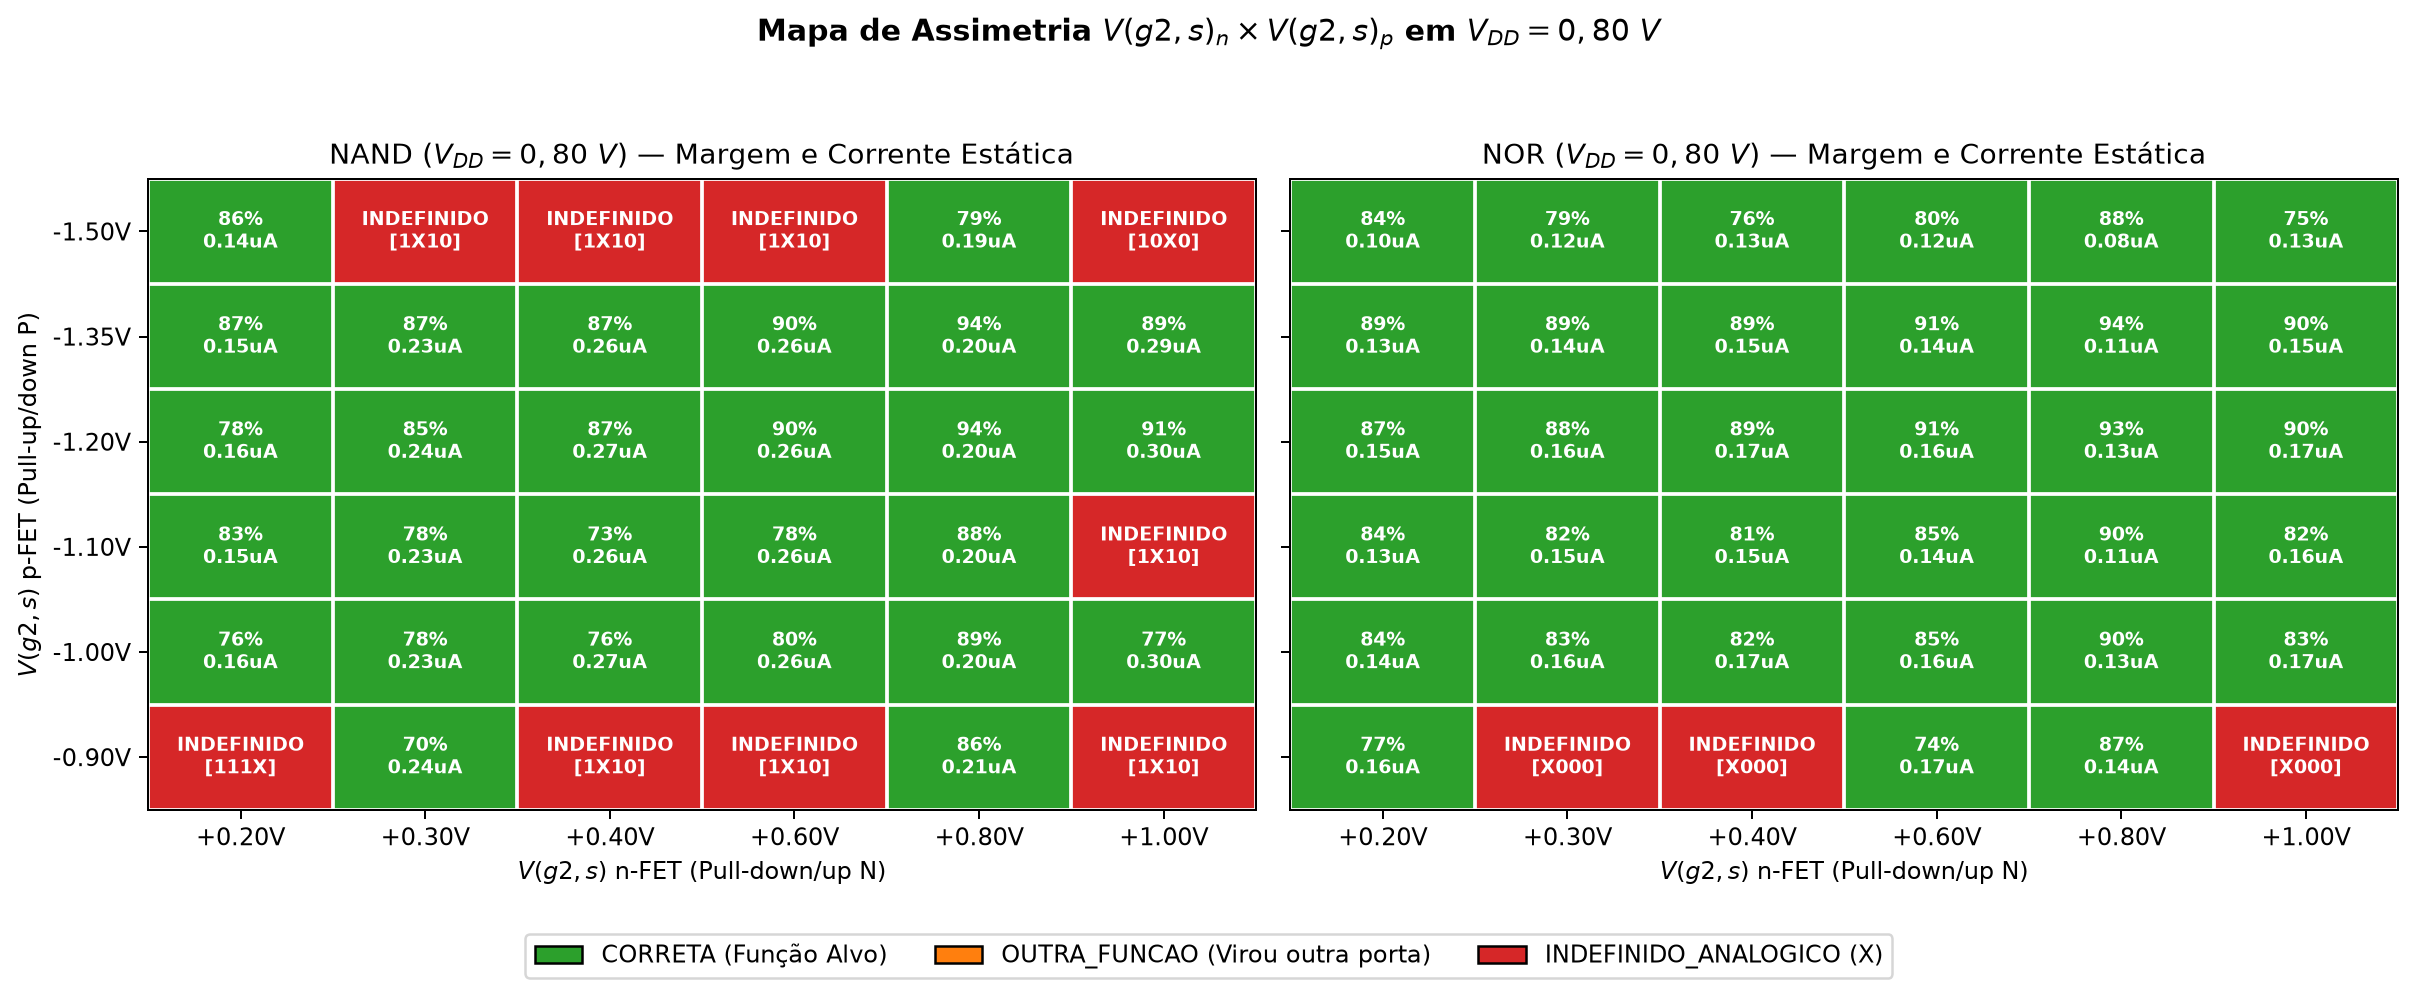
\includegraphics[width=0.92\textwidth]{m06_nand_nor_assimetria_vg2.png}
\caption{Mapa de assimetria $V(g2,s)_n \times V(g2,s)_p$ em $V_{DD}=0{,}80\ \text{V}$ para \texttt{NAND} e \texttt{NOR}, evidenciando a degrada\c{c}\~{a}o n\~{a}o monot\^{o}nica em $V(g2,s)_p = -1{,}50\ \text{V}$.}
\label{fig:m06_nn_asym}
\end{figure}

\begin{figure}[htbp]
\centering
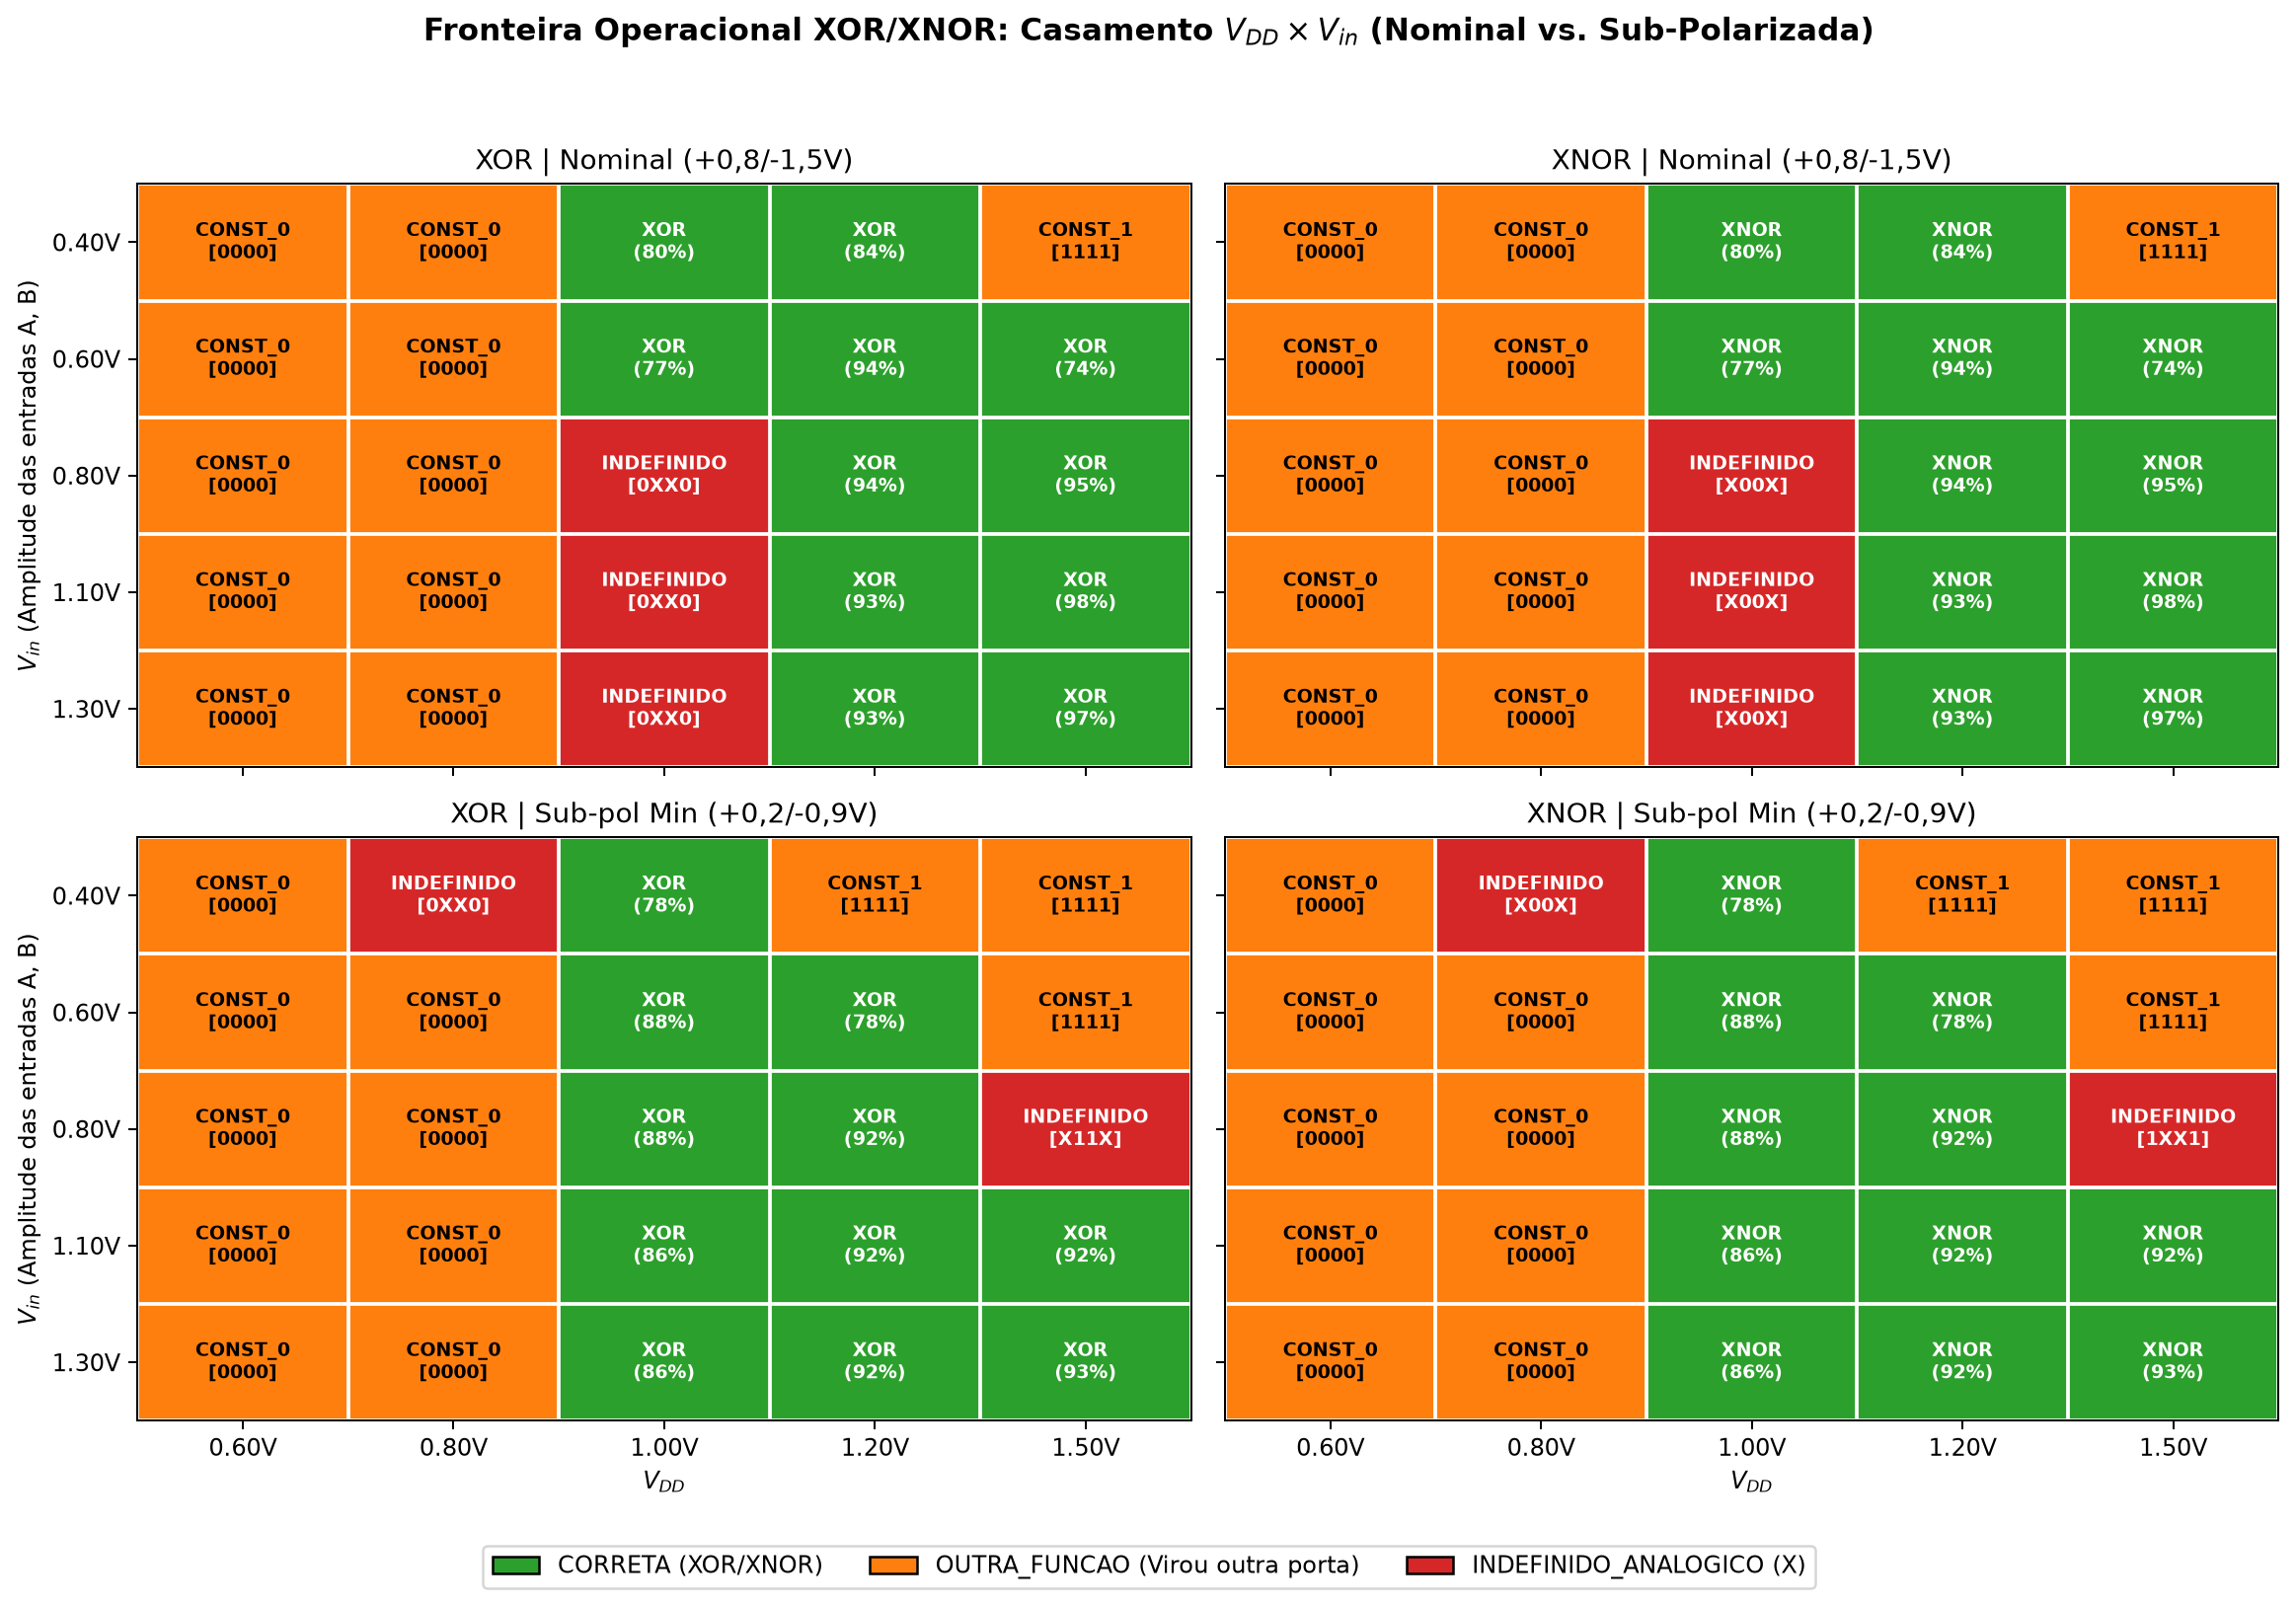
\includegraphics[width=0.92\textwidth]{m06_xor_xnor_mapa_vdd_vin.png}
\caption{Mapa operacional $V_{DD} \times V_{\mathrm{in}}$ da porta \texttt{XOR}/\texttt{XNOR} sob polaridade nominal, sub-polariza\c{c}\~{a}o e porta fixa, expondo as zonas \texttt{CONST\_0}, \texttt{CONST\_1} e indefinida.}
\label{fig:m06_xor_mapa}
\end{figure}

\subsection{Assimetria DPA em Sete Tuplas Polim\'{o}rficas e \textit{Benchmark} do Full Adder}\label{sec:res_tuplas}

No M\'{o}dulo \texttt{07}, todas as $72$ combina\c{c}\~{o}es de entrada e chave avaliadas sobre as sete tuplas atingiram $100{,}0\%$ de corretude l\'{o}gica ($V_{1,\min} \ge 0{,}6792\ \text{V}$ em $0{,}8\ \text{V}$ e $\ge 1{,}3767\ \text{V}$ em $1{,}5\ \text{V}$; $V_{0,\max} \le 0{,}0128\ \text{V}$). A Tabela~\ref{tab:tuplas_dpa} consolida integralmente as m\'{e}tricas de custo, seguran\c{c}a DPA, desempenho din\^{a}mico e robustez Monte Carlo.

\begin{table}[htbp]
\centering
\caption{M\'{e}tricas consolidadas de custo, assimetria DPA, desempenho e robustez Monte Carlo nas sete tuplas polim\'{o}rficas ($C_{\mathrm{load}} = 0{,}3\ \text{fF}$).}
\label{tab:tuplas_dpa}
\resizebox{\textwidth}{!}{%
\begin{tabular}{l c c c c c c c c c c c c}
\toprule
\textbf{Tupla} & \textbf{N\'{u}c./Tot.} & $\sum W$ ($\mu\text{m}$) & $V_{DD}$ (V) & $I_{\mathrm{pico}}$ M0/M1 ($\mu\text{A}$) & \textbf{DPA Pico} & \textbf{DPA M\'{e}d.} & $t_p$ (ps) & $P_{\mathrm{m\acute{e}d}}$ (nW) & $E_{\mathrm{sw}}$ (fJ) & \textbf{PDP} (aJ) & \textbf{MC} ($N=250$) \\
\midrule
\texttt{(NAND, NOR)}   & 4T / 4T   & $6{,}0$  & $0{,}8$ & $0{,}5643$ / $0{,}2138$ & $163{,}91\%$ & $44{,}62\%$ & $554{,}28$ & $40{,}17$  & $0{,}5022$ & $22{,}27$ & $100{,}00\%$ \\
\texttt{(XOR, XNOR)}   & 4T / 8T   & $4{,}0$  & $1{,}5$ & $1{,}6914$ / $1{,}6914$ & $0{,}00\%$   & $30{,}57\%$ & $151{,}84$ & $102{,}47$ & $1{,}2808$ & $15{,}56$ & $100{,}00\%$ \\
\texttt{(AND, OR)}     & 6T / 6T   & $9{,}0$  & $0{,}8$ & $1{,}7345$ / $1{,}8394$ & $6{,}05\%$   & $30{,}87\%$ & $454{,}27$ & $48{,}04$  & $0{,}6005$ & $21{,}82$ & $100{,}00\%$ \\
\texttt{(NAND, XNOR)}  & 6T / 10T  & $8{,}0$  & $1{,}5$ & $1{,}7050$ / $1{,}3387$ & $27{,}36\%$  & $73{,}87\%$ & $163{,}46$ & $94{,}14$  & $1{,}1768$ & $15{,}39$ & $100{,}00\%$ \\
\texttt{(NOR, XOR)}    & 6T / 10T  & $8{,}0$  & $1{,}5$ & $1{,}7129$ / $1{,}6932$ & $1{,}16\%$   & $29{,}60\%$ & $144{,}87$ & $121{,}49$ & $1{,}5186$ & $17{,}60$ & $100{,}00\%$ \\
\texttt{(AOI21, OAI21)}& 6T / 6T   & $12{,}0$ & $0{,}8$ & $0{,}6810$ / $0{,}4299$ & $58{,}44\%$  & $19{,}22\%$ & $555{,}72$ & $59{,}97$  & $0{,}4498$ & $33{,}33$ & $99{,}55\%$  \\
\texttt{(MAJ3, XOR3)}  & 10T / 18T & $18{,}0$ & $1{,}5$ & $1{,}4360$ / $1{,}4355$ & $0{,}04\%$   & $47{,}08\%$ & $180{,}71$ & $212{,}44$ & $1{,}9119$ & $38{,}39$ & $100{,}00\%$ \\
\bottomrule
\end{tabular}}
\end{table}

Sob o testbench padronizado no \texttt{ngspice-47}, as assinaturas de corrente (Figura~\ref{fig:m07_assinaturas}) e a fronteira de Pareto (Figura~\ref{fig:m07_pareto}) revelam compromissos claros de projeto:
\begin{itemize}
    \item \texttt{(NAND, NOR)} apresenta o menor custo f\'{i}sico ($4\text{T}$, $40{,}17\ \text{nW}$), por\'{e}m sofre elevada exposi\c{c}\~{a}o de pico DPA ($163{,}91\%$) e atraso elevado ($554{,}28\ \text{ps}$) devido \`{a} assimetria entre redes paralela ($W=1{,}0$) e s\'{e}rie ($W=2{,}0$).
    \item \texttt{(XOR, XNOR)} elimina integralmente a assimetria de pico ($0{,}00\%$, $1{,}6914\ \mu\text{A}$ em ambos os modos) mantendo $\mathrm{PDP} = 15{,}56\ \text{aJ}$.
    \item Em \texttt{(AND, OR)}, a adi\c{c}\~{a}o do inversor \texttt{BP\_INV08} ($+2\text{T}$) desacopla a carga da rede polim\'{o}rfica e reduz a assimetria global de pico na alimenta\c{c}\~{a}o para $6{,}05\%$, embora a assimetria espec\'{i}fica das transi\c{c}\~{o}es $1 \to 0$ permane\c{c}a alta ($116{,}90\%$).
    \item Entre as c\'{e}lulas mistas, \texttt{(NOR, XOR)} destaca-se como excelente compromisso para \textit{logic locking} heterog\^{e}neo ($1{,}16\%$ de assimetria de pico e menor atraso m\'{e}dio da su\'{i}te: $144{,}87\ \text{ps}$), enquanto \texttt{(NAND, XNOR)} exibe alta assimetria m\'{e}dia ($73{,}87\%$) pelo desbalanceamento de ocorr\^{e}ncia de \texttt{'1'} na tabela da \texttt{NAND} ($75\%$) frente \`{a} \texttt{XNOR} ($50\%$).
    \item Nas portas de tr\^{e}s entradas, \texttt{(AOI21, OAI21)} alcan\c{c}a a menor assimetria m\'{e}dia ($19{,}22\%$) e menor energia de chaveamento ($0{,}4498\ \text{fJ}$) em $6\text{T}$, com pequena redu\c{c}\~{a}o de taxa de acerto Monte Carlo ($99{,}55\%$, Figura~\ref{fig:m07_mc}) por empilhamento em \texttt{OAI21}; j\'{a} \texttt{(MAJ3, XOR3)} estende o equil\'{i}brio quad-sim\'{e}trico a tr\^{e}s entradas com $0{,}04\%$ de DPA de pico e $100{,}0\%$ de acerto estat\'{i}stico.
\end{itemize}

\begin{figure}[htbp]
\centering
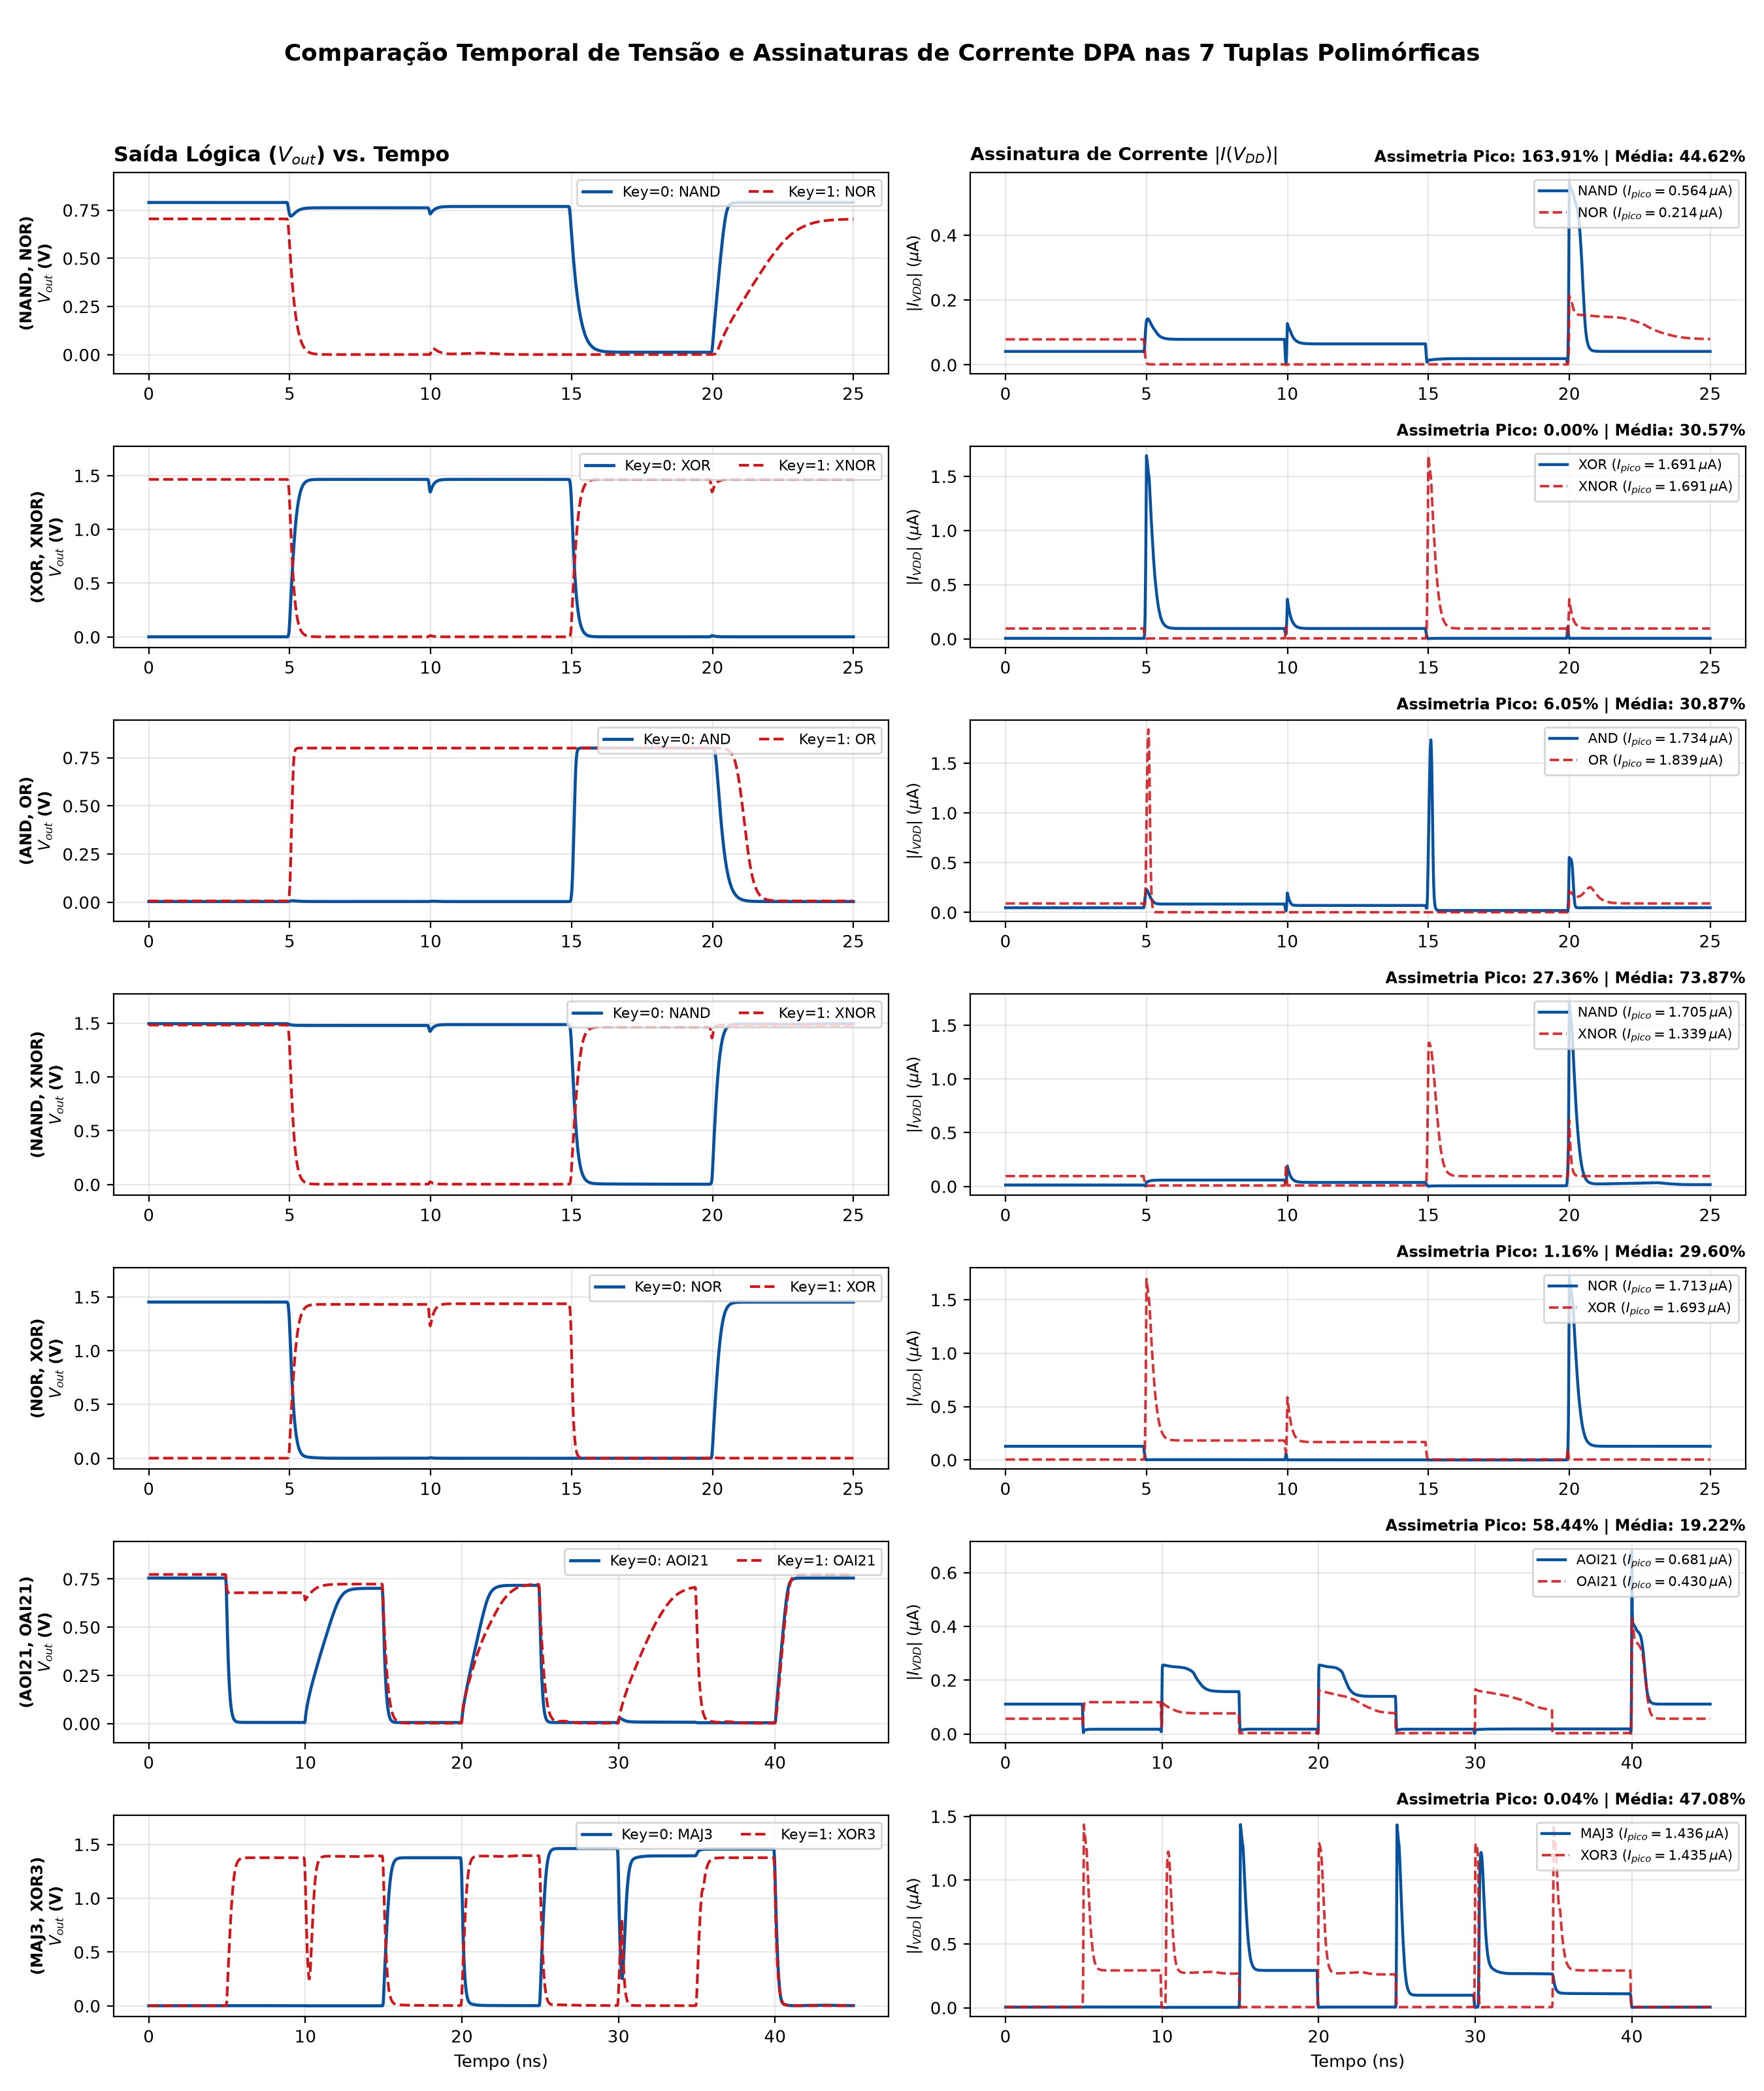
\includegraphics[width=0.90\textwidth,height=0.76\textheight,keepaspectratio]{m07_assinaturas_corrente_tuplas.png}
\caption{Assinaturas temporais de corrente $|I(V_{DD})|$ comparando $\text{Key}=0$ e $\text{Key}=1$ nas sete tuplas polim\'{o}rficas sob carga padronizada ($C_{\mathrm{load}} = 0{,}3\ \text{fF}$).}
\label{fig:m07_assinaturas}
\end{figure}

\begin{figure}[htbp]
\centering
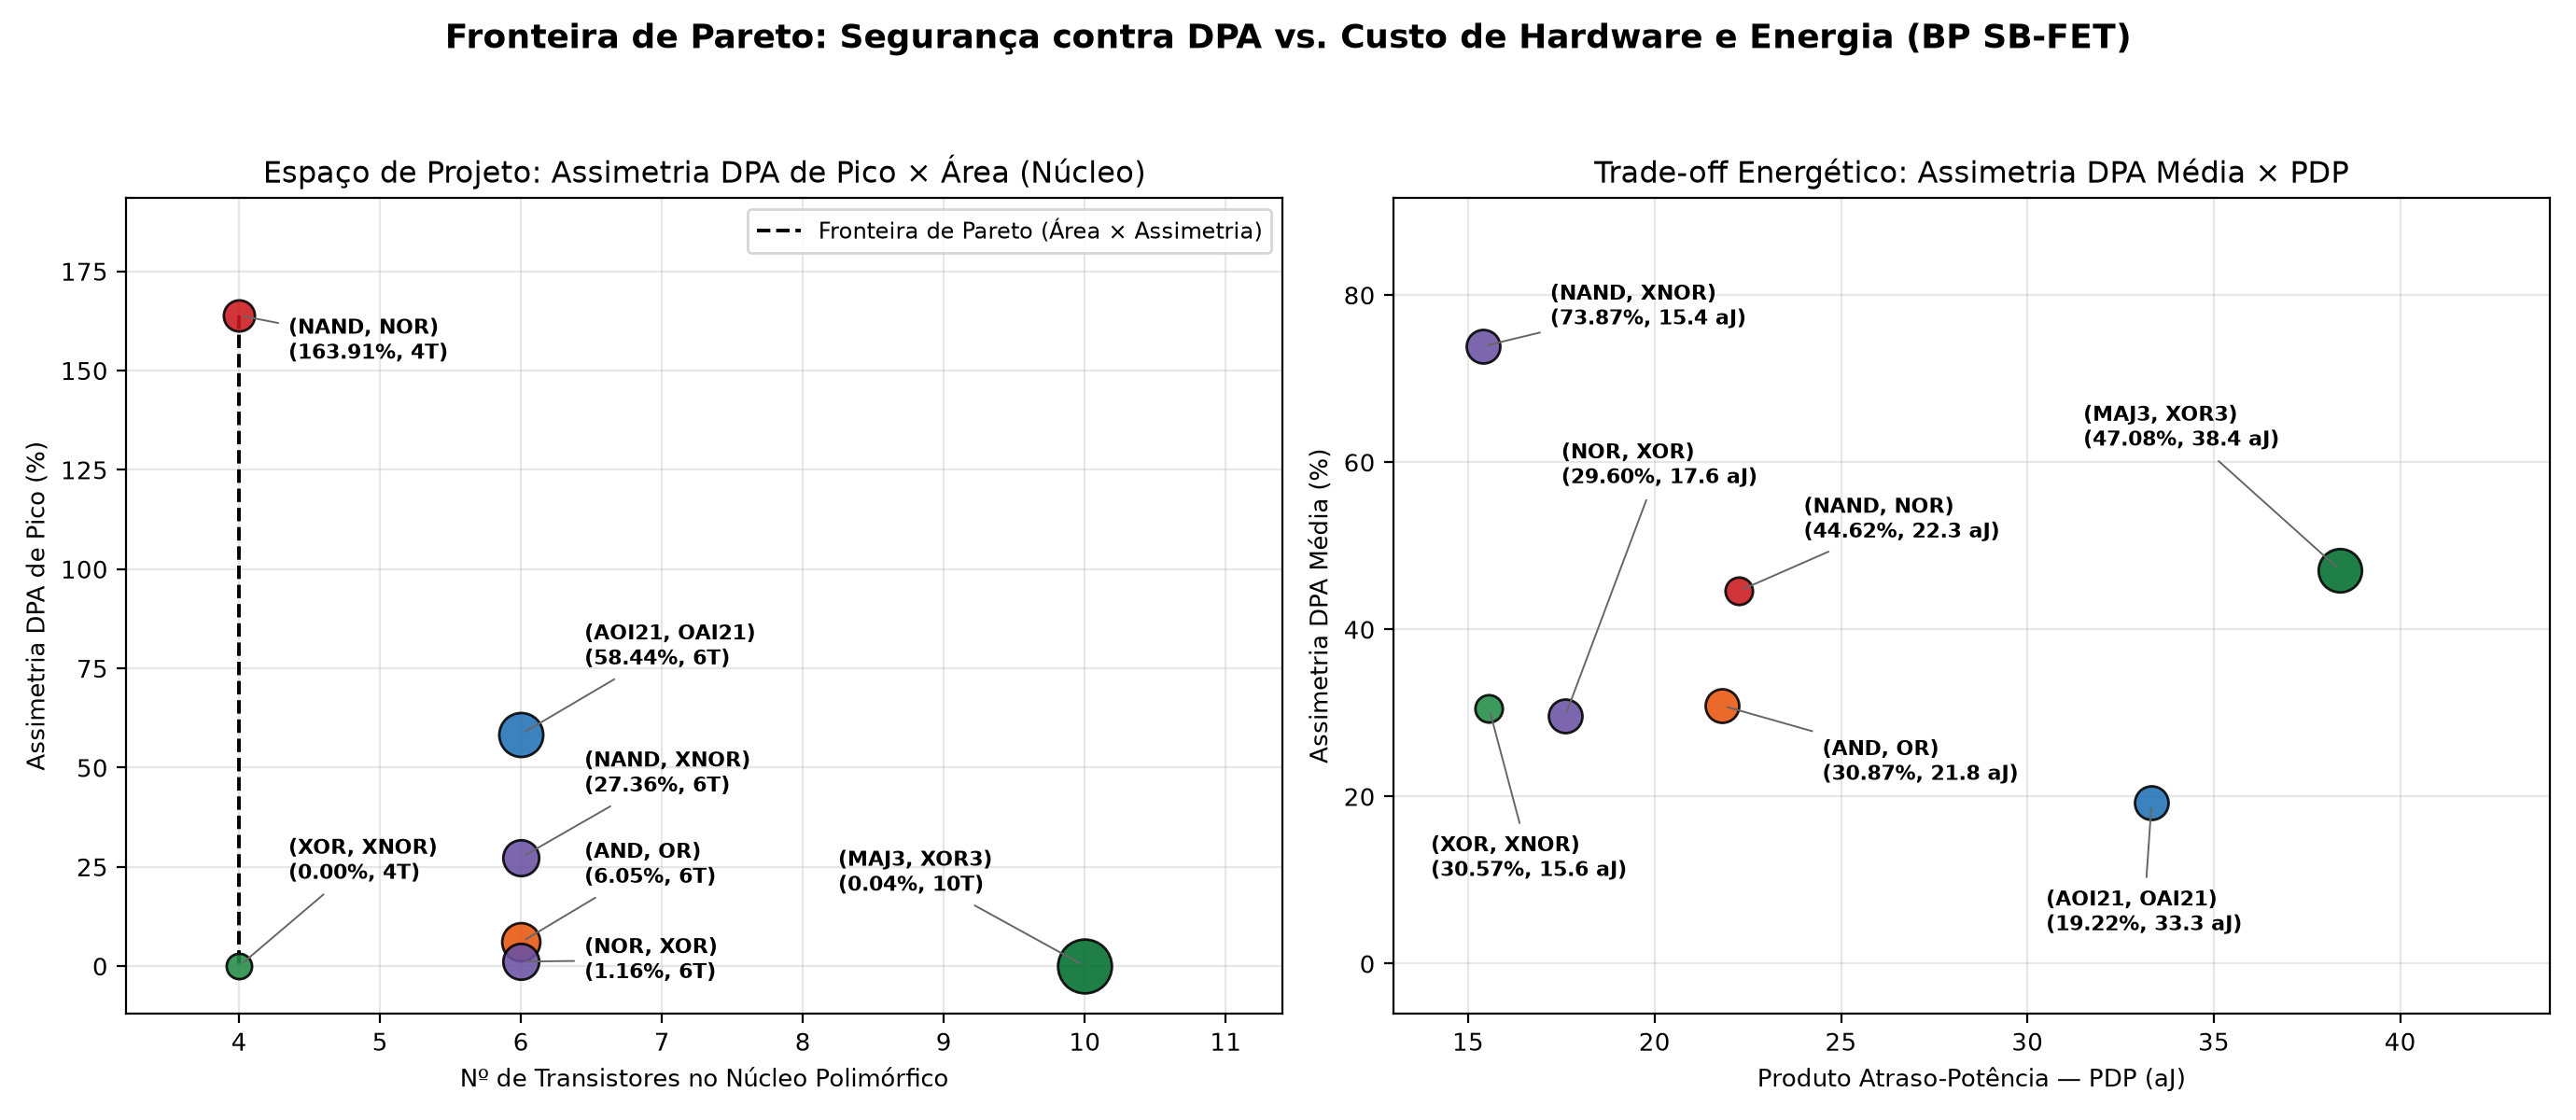
\includegraphics[width=0.92\textwidth]{m07_pareto_assimetria_vs_custo.png}
\caption{Fronteira de Pareto relacionando assimetria DPA de pico, n\'{u}mero de transistores e produto pot\^{e}ncia-atraso ($\mathrm{PDP}$) nas sete tuplas avaliadas.}
\label{fig:m07_pareto}
\end{figure}

\begin{figure}[htbp]
\centering
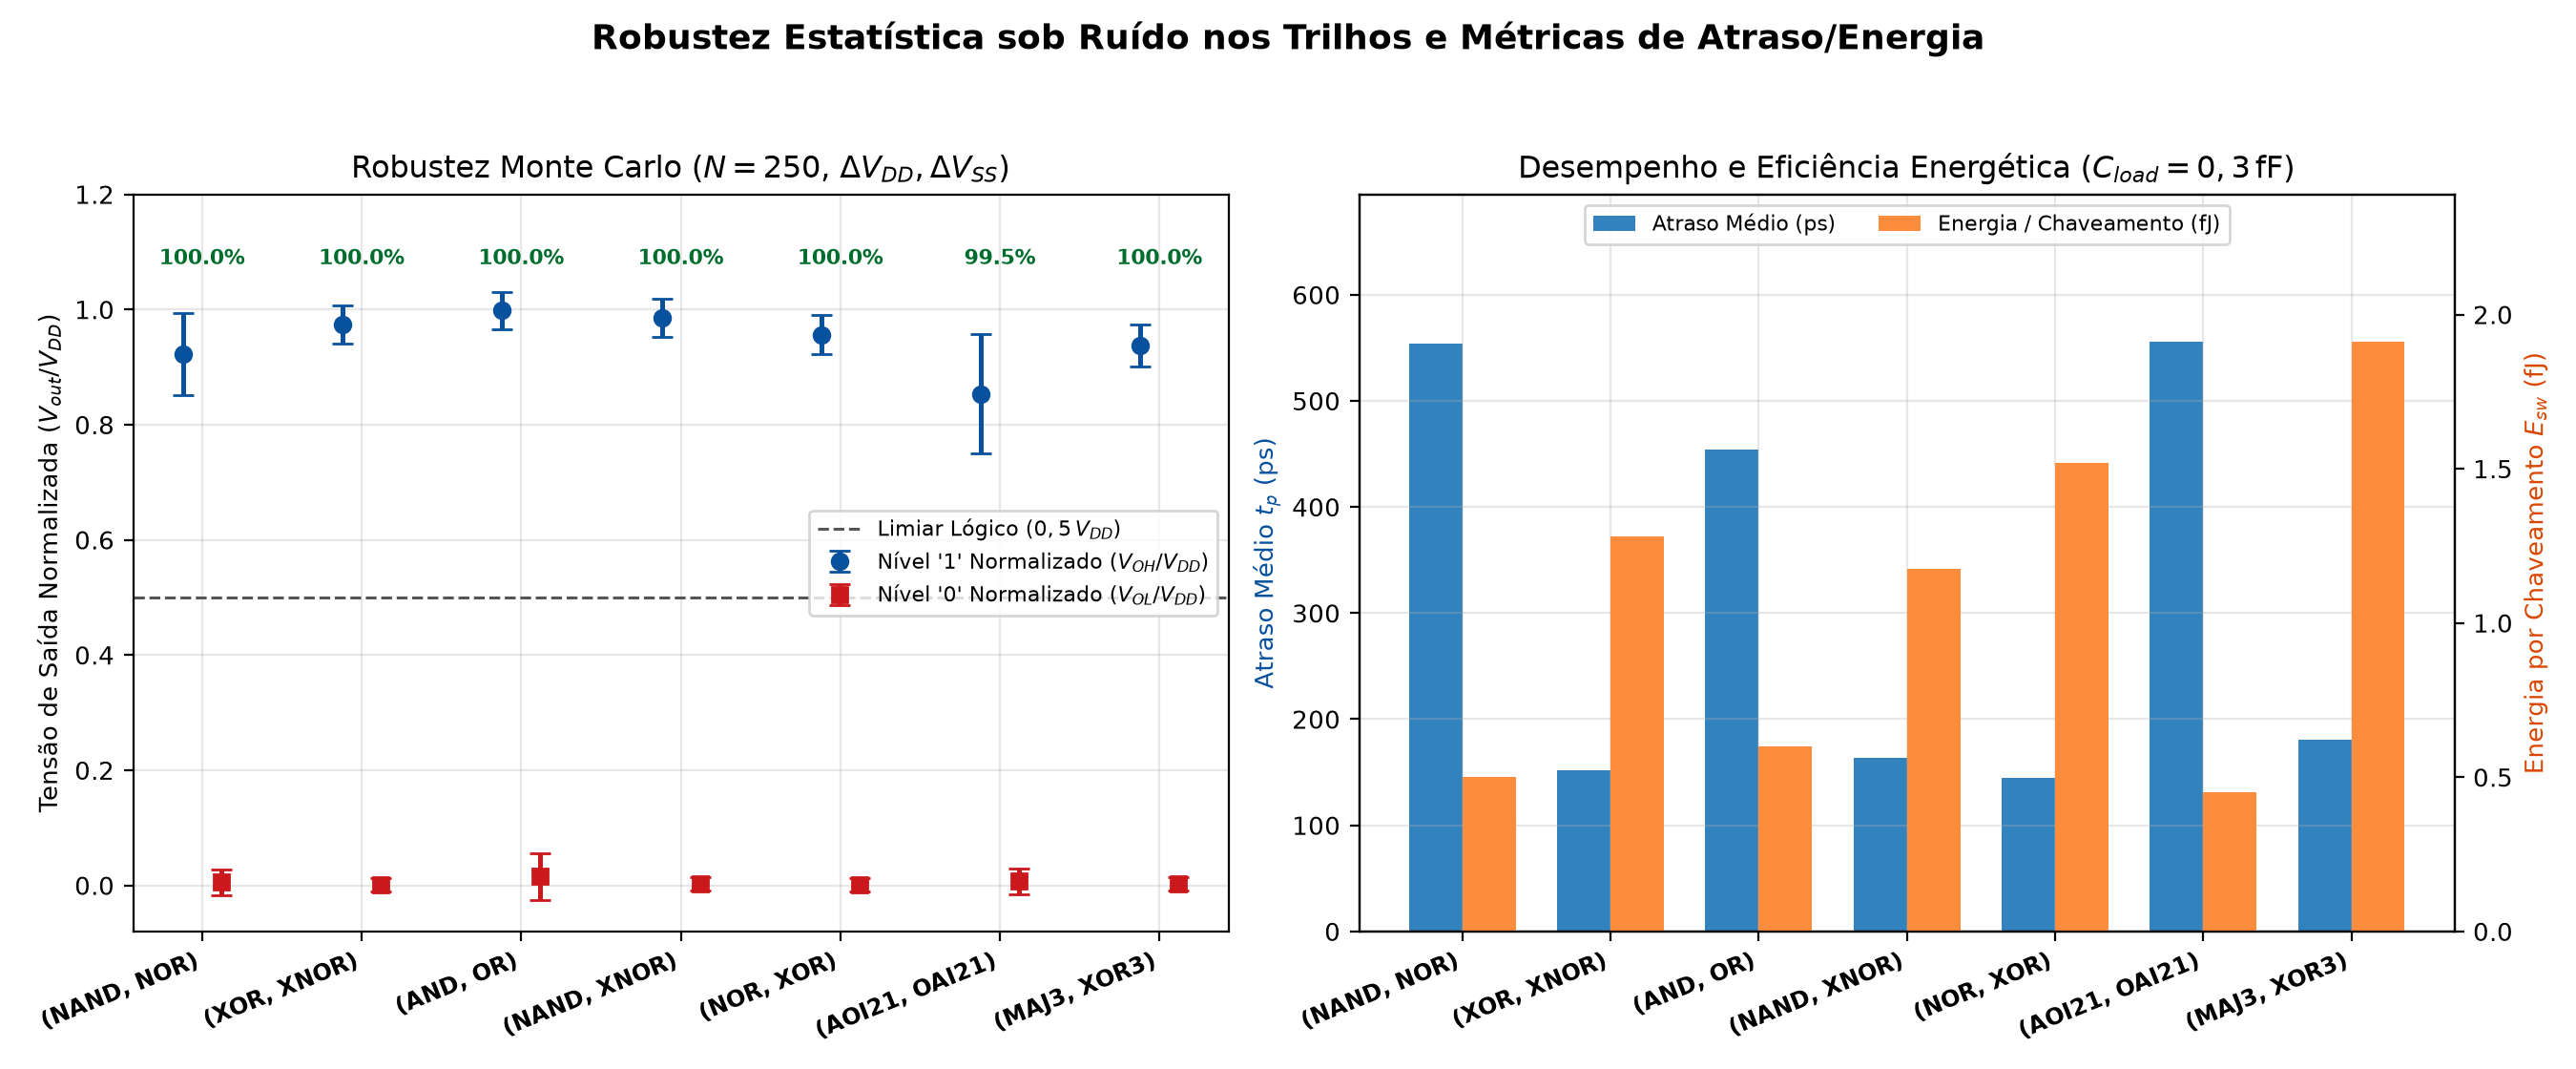
\includegraphics[width=0.92\textwidth]{m07_robustez_montecarlo_tuplas.png}
\caption{Taxa de acerto em Monte Carlo ($N=250$) sobre grade real de ru\'{i}do nos trilhos e distribui\c{c}\~{a}o de atraso e energia entre as sete tuplas.}
\label{fig:m07_mc}
\end{figure}

No \textit{benchmark} de sistema com tr\^{e}s arquiteturas de Somador Completo 1-bit (Tabela~\ref{tab:fa_perfis} e Figura~\ref{fig:m07_fa}), todos os perfis obtiveram $100{,}0\%$ de corretude funcional em $K=00$. O \textbf{Perfil 2} (baseado em tr\^{e}s portas \texttt{NAND}/\texttt{NOR} no \textit{carry}) eleva a contagem para 28T, multiplica o atraso cr\'{i}tico em $3{,}58\times$ frente ao Baseline ($177{,}72 \to 636{,}68\ \text{ps}$), aumenta o PDP cr\'{i}tico em $3{,}54\times$ ($131{,}86 \to 466{,}44\ \text{aJ}$) e exp\~{o}e uma assinatura DPA de $113{,}83\%$ no caminho de \textit{carry}. Em contrapartida, o \textbf{Perfil 3} substitui a \'{a}rvore \texttt{NAND}/\texttt{NOR} por uma \'{u}nica c\'{e}lula \texttt{(MAJ3, XOR3)} de 10T, reduzindo a contagem de n\'{u}cleo para 26T, elevando a Dist\^{a}ncia de Hamming em chave errada ($K=11$) de $68{,}75\%$ para $87{,}50\%$ e derrubando a assimetria DPA de pico no est\'{a}gio polim\'{o}rfico de $113{,}83\%$ para apenas \textbf{$0{,}04\%$}. Com atraso cr\'{i}tico de $196{,}98\ \text{ps}$ ($+10{,}8\%$ sobre o Baseline) e PDP de $155{,}19\ \text{aJ}$ ($+17{,}7\%$ sobre o Baseline e \textbf{$3{,}01\times$ inferior ao Perfil 2}), o Perfil 3 demonstra superioridade simult\^{a}nea em seguran\c{c}a, \'{a}rea e efici\^{e}ncia energ\'{e}tica.

\begin{table}[htbp]
\centering
\caption{\textit{Benchmark} arquitetural do Somador Completo 1-bit em tr\^{e}s perfis no \texttt{ngspice-47} ($C_{\mathrm{load}} = 0{,}3\ \text{fF}$).}
\label{tab:fa_perfis}
\resizebox{\textwidth}{!}{%
\begin{tabular}{l c c c c c c c c c}
\toprule
\textbf{Perfil Arquitetural} & \textbf{N\'{u}cleo} & $\sum W$ & \textbf{Corret.\ K00} & \textbf{HD (K11)} & $t_{\mathrm{cr\acute{i}t}}$ (ps) & $P_{\mathrm{m\acute{e}d}}$ (nW) & \textbf{PDP} (aJ) & \textbf{DPA Pico Carry} & \textbf{DPA M\'{e}d.\ Carry} \\
\midrule
1. Baseline (Comum, sem \textit{lock}) & 20T & $24{,}0$ & $100{,}0\%$ & $0{,}0\%$   & $177{,}72$ & $741{,}97$ & $131{,}86$ & N/A & N/A \\
2. Custo/Desempenho (\texttt{NAND}/\texttt{NOR}) & 28T & $38{,}0$ & $100{,}0\%$ & $68{,}75\%$ & $636{,}68$ & $732{,}60$ & $466{,}44$ & $113{,}83\%$ & $62{,}44\%$ \\
3. Baixa Assimetria (\texttt{MAJ3}/\texttt{XOR3}) & 26T & $38{,}0$ & $100{,}0\%$ & $87{,}50\%$ & $196{,}98$ & $787{,}87$ & $155{,}19$ & $0{,}04\%$   & $47{,}47\%$ \\
\bottomrule
\end{tabular}}
\end{table}

\begin{figure}[htbp]
\centering
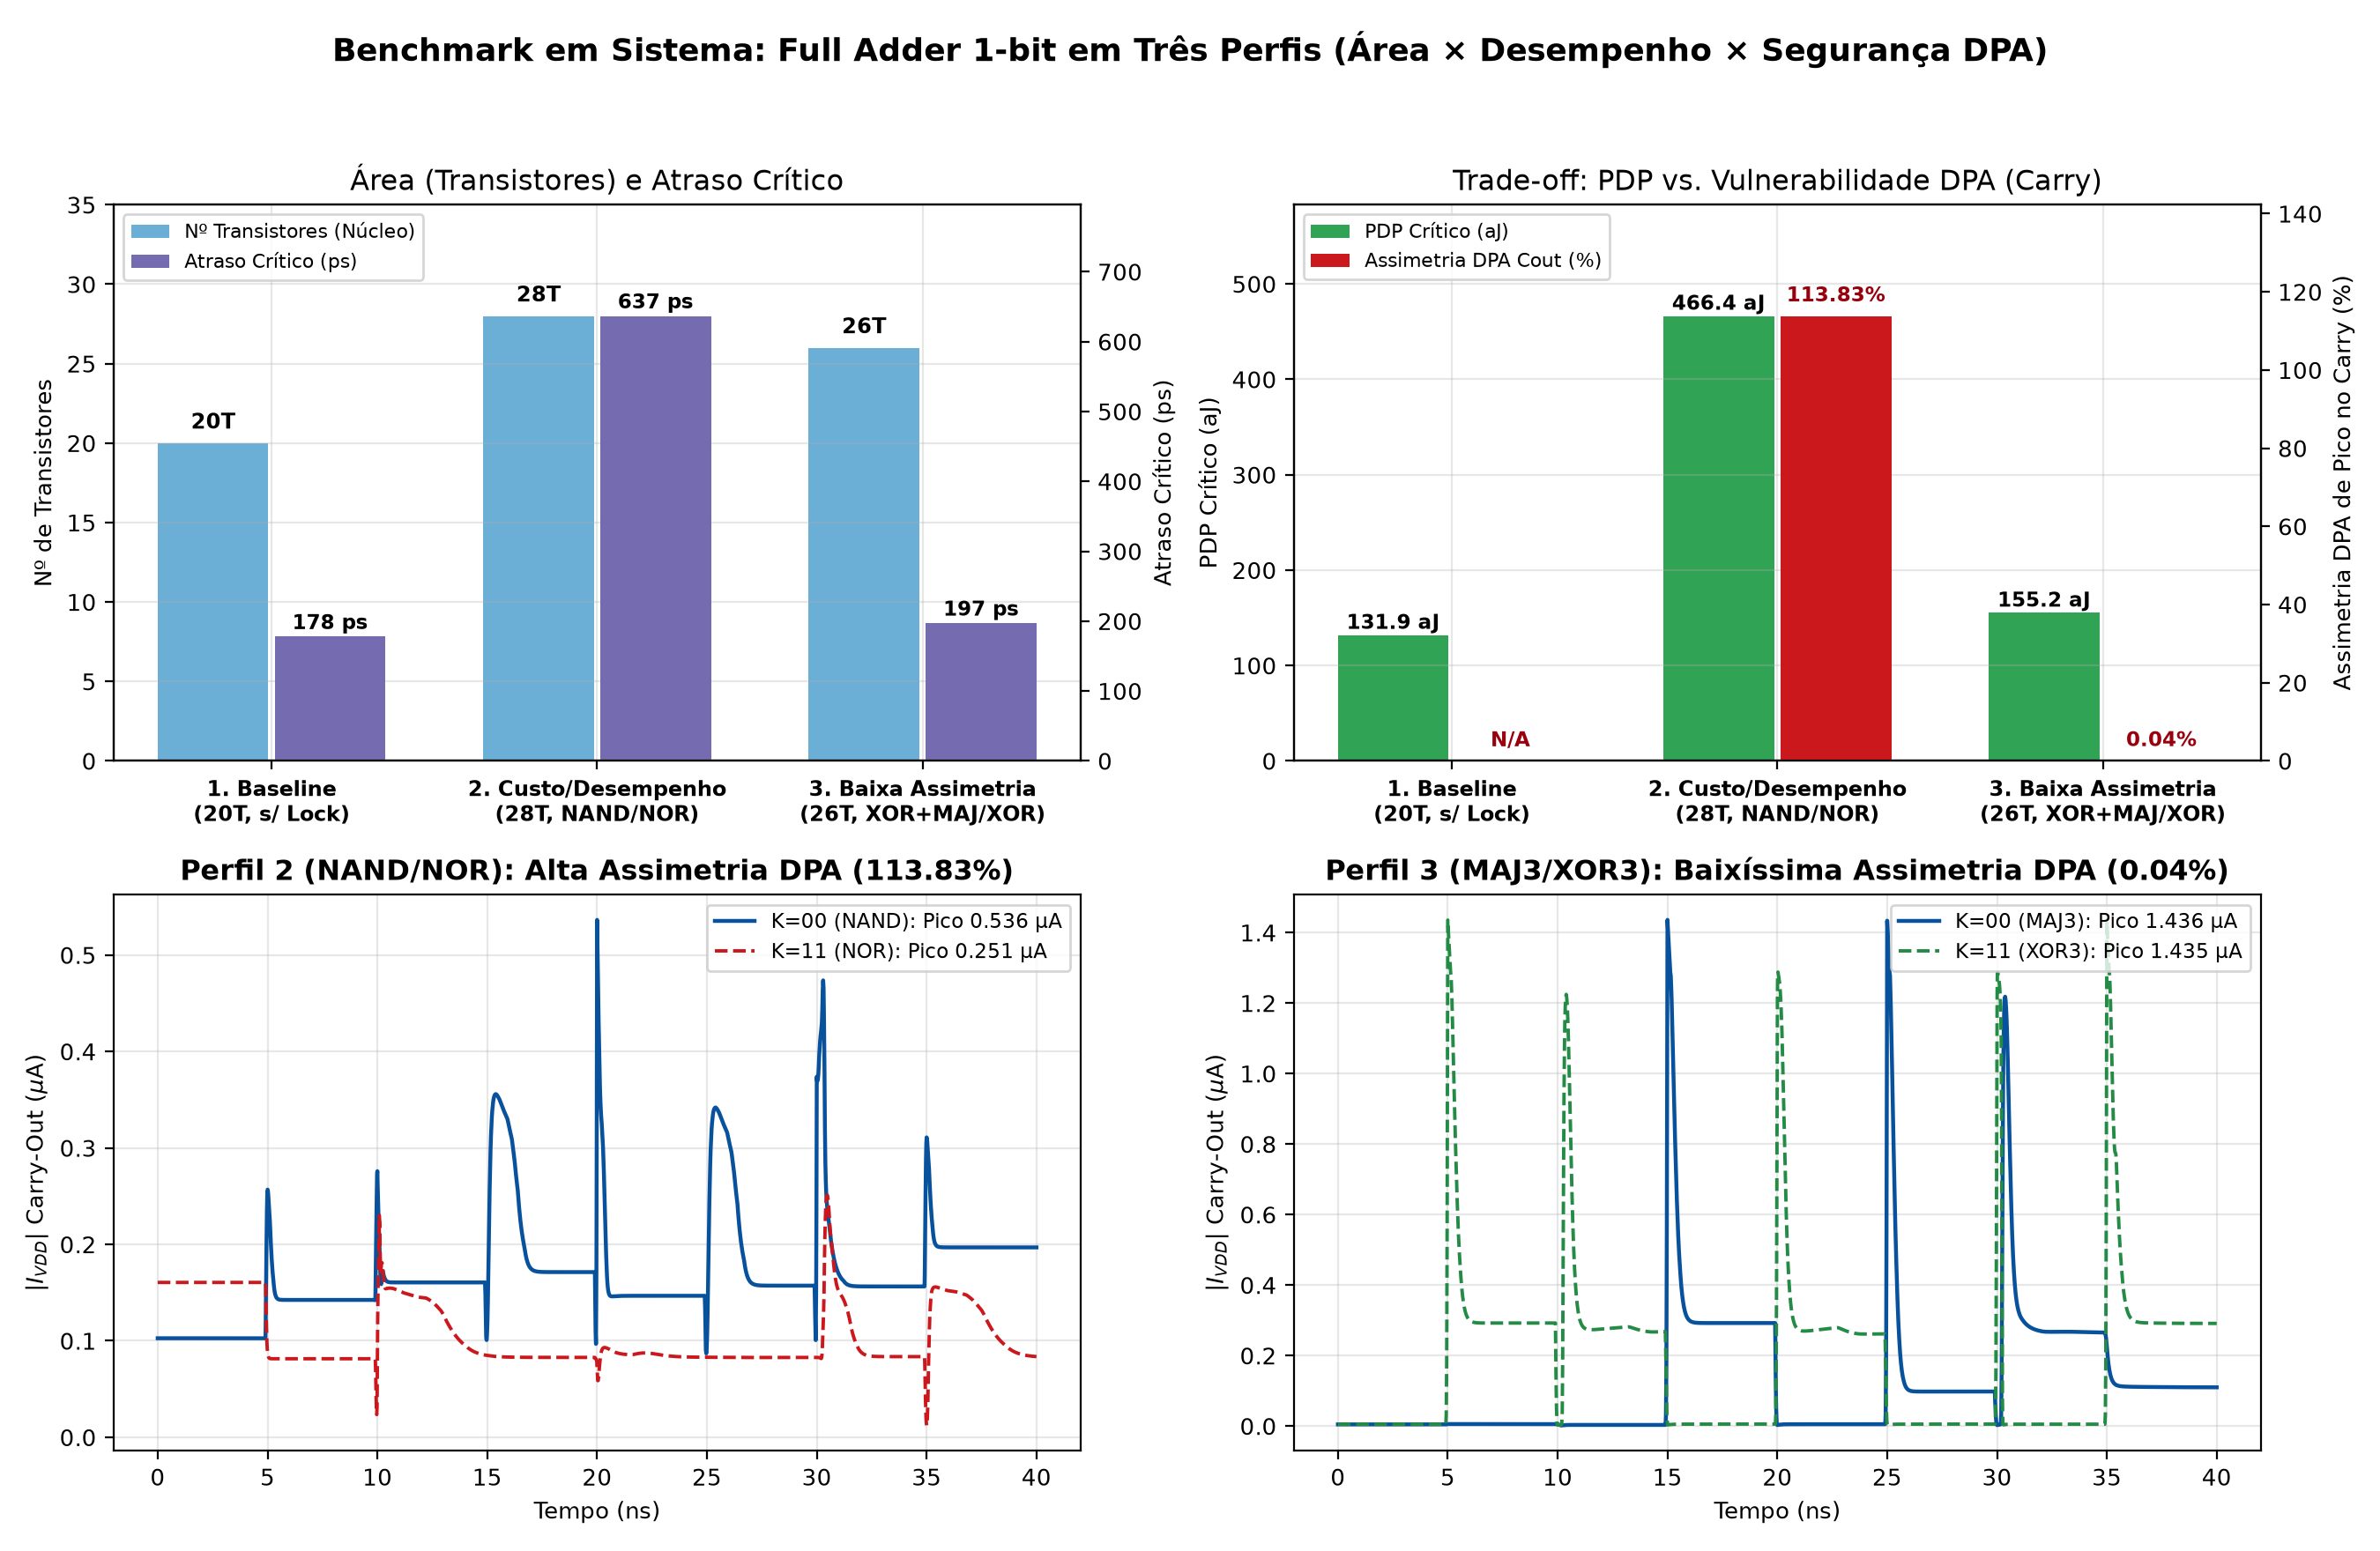
\includegraphics[width=0.92\textwidth]{m07_benchmark_full_adder_perfis.png}
\caption{Comparativo do Somador Completo 1-bit nos tr\^{e}s perfis arquiteturais quanto a contagem de transistores, atraso cr\'{i}tico, PDP, ofusca\c{c}\~{a}o (HD) e assimetria DPA no \textit{carry}.}
\label{fig:m07_fa}
\end{figure}

\subsection{Valida\c{c}\~{a}o Ponta a Ponta do Simulador Visual Interativo (\textit{BP-FET Studio})}\label{sec:res_web}

A su\'{i}te automatizada \texttt{simulador\_web/test\_simulator.py} validou integralmente a compila\c{c}\~{a}o de grafos, a simula\c{c}\~{a}o em lote no \texttt{ngspice-47} e o servidor REST da plataforma \textit{BP-FET Studio}:
\begin{enumerate}
    \item \textbf{Sete tuplas polim\'{o}rficas e inversor \texttt{INV} em alto n\'{i}vel:} todas as combina\c{c}\~{o}es de tabela-verdade e o mapeamento interno de transistores do modo \textit{Raio-X} passaram com $100\%$ de exatid\~{a}o, reproduzindo os valores de assimetria DPA de pico do M\'{o}dulo \texttt{07} (\texttt{NAND\_NOR}: $163{,}91\%$; \texttt{XOR\_XNOR}: $0{,}00\%$; \texttt{AND\_OR}: $6{,}05\%$; \texttt{NAND\_XNOR}: $27{,}36\%$; \texttt{NOR\_XOR}: $1{,}16\%$; \texttt{AOI21\_OAI21}: $58{,}44\%$; \texttt{MAJ3\_XOR3}: $0{,}04\%$; \texttt{INV}: $0{,}00\%$) em tempos de execu\c{c}\~{a}o entre $234\ \text{ms}$ (\texttt{INV}) e $7{,}04\ \text{s}$ (\texttt{MAJ3\_XOR3}).
    \item \textbf{Oito templates do cat\'{a}logo:} todos os modelos em alto e baixo n\'{i}vel foram simulados com sucesso ($0{,}65\ \text{s}$ a $14{,}31\ \text{s}$), verificando tanto os Somadores Completos dos Perfis 2 e 3 em $K=0$, quanto a invers\~{a}o f\'{i}sica de polaridade (\textit{p-FET} $\leftrightarrow$ \textit{n-FET}) na c\'{e}lula \texttt{NAND}/\texttt{NOR} 4T e a reten\c{c}\~{a}o ($\Delta V > 0{,}7\ \text{V}$ em $12\ \text{ns}$, \texttt{XPU1} como \textit{p-FET}) seguida de colapso ($\Delta V < 0{,}25\ \text{V}$ em $28\ \text{ns}$, \texttt{XPU1} como \textit{n-FET}) na SRAM 6T.
    \item \textbf{Cascata mista multidom\'{i}nio e API HTTP:} um circuito arbitr\'{a}rio encadeando $0{,}8\ \text{V} \to 1{,}5\ \text{V} \to 0{,}8\ \text{V}$ (\texttt{NAND\_\allowbreak NOR} $\to$ \texttt{XOR\_\allowbreak XNOR} $\to$ \texttt{AND\_\allowbreak OR}) com condicionamento autom\'{a}tico de n\'{i}vel foi compilado e validado em $5{,}87\ \text{s}$ ($100\%$ exato em $\text{Key}=0$ e $\text{Key}=1$), e todas as rotas HTTP/JSON (\texttt{/}, \texttt{/api/\allowbreak tuples}, \texttt{/api/\allowbreak templates}, \texttt{/api/\allowbreak simulate}) responderam com c\'{o}digo $200$.
\end{enumerate}

\section{Conclus\~{a}o}\label{sec:conclusao}

Este trabalho estabeleceu e validou um ecossistema computacional completo e de c\'{o}digo aberto em \texttt{ngspice-47} e Python para modelagem, caracteriza\c{c}\~{a}o f\'{i}sica, an\'{a}lise de seguran\c{c}a de hardware e prototipagem visual de circuitos digitais baseados em transistores bidimensionais BP SB-FET. A tradu\c{c}\~{a}o da superf\'{i}cie experimental 4D com refer\^{e}ncia bilateral de fonte e curvas de satura\c{c}\~{a}o espec\'{i}ficas por porta (\texttt{bp\_ari\_ngspice.lib} \texttt{v2}) eliminou a depend\^{e}ncia propriet\'{a}ria do Synopsys HSPICE/Verilog-A com erro m\'{e}dio inferior a $0{,}0621\%$ frente \`{a}s tabelas originais, alcan\c{c}ou $R^2 \ge 0{,}99977$ nos regimes \texttt{N\_transfer}, \texttt{P\_transfer} e \texttt{P\_output} e reduziu em $196\times$ o RMSE de sa\'{i}da \textit{p-FET} ao incorporar o regime real medido em $V_{g2} = -1{,}5\ \text{V}$.

Em n\'{i}vel de circuito e seguran\c{c}a, os experimentos demonstraram que a compensa\c{c}\~{a}o eletrost\'{a}tica de $V_{fb}$ preserva ganho diferencial superior \`{a} unidade ($|A_v| = 2{,}71$) e excurs\~{a}o de $89{,}75\%$ no inversor complementar at\'{e} $V_{DD} = 0{,}2\ \text{V}$. As primitivas polim\'{o}rficas \texttt{NAND}/\texttt{NOR} e \texttt{XOR}/\texttt{XNOR} alcan\c{c}aram $100\%$ de acur\'{a}cia em comuta\c{c}\~{a}o din\^{a}mica com $0\%$ de sobrecarga de transistores, mantendo $100{,}0\%$ de corretude l\'{o}gica em $250$ amostras Monte Carlo de flutua\c{c}\~{a}o de trilhos. Na c\'{e}lula SRAM 6T, comprovou-se a viabilidade do Mecanismo B sob alimenta\c{c}\~{a}o fixa: a sintonia de $V_{g2,\mathrm{PU}} = -0{,}2\ \text{V}$ garantiu $\Delta V_{\mathrm{Key0}} = 0{,}9747\ \text{V}$ e $\mathrm{SNM}_{\mathrm{Hold}} = 167{,}12\ \text{mV}$ na chave autorizada, enquanto $\text{Key}=1$ colapsou a reten\c{c}\~{a}o para $\mathrm{SNM} = 0{,}00\ \text{mV}$ ($\Delta V_{\mathrm{Key1}} = 0{,}0762\ \text{V}$), com mitiga\c{c}\~{a}o de \textit{Read Disturb} via \textit{Wordline Underdrive Read-Assist} ($\mathrm{SNM}_{\mathrm{Read,Assist}} = 66{,}23\ \text{mV}$ em $\mathrm{WL}=0{,}30\ \text{V}$).

A investiga\c{c}\~{a}o das fronteiras operacionais fora do ponto nominal confirmou a ocorr\^{e}ncia de tr\^{e}s fen\^{o}menos cr\'{i}ticos dentro do dom\'{i}nio experimental das LUTs: al\'{e}m de faixas robustas de opera\c{c}\~{a}o correta e travamentos degenerados (\texttt{CONST\_0} em sub-tens\~{a}o e \texttt{CONST\_1} por \textit{overdrive} assim\'{e}trico em \texttt{XOR}/\texttt{XNOR}), demonstrou-se uma convers\~{a}o espont\^{a}nea \texttt{NAND} $\to$ \texttt{NOR} sem troca de chave em $V_{DD}=0{,}65\ \text{V}$ ($+0{,}4/-1{,}1\ \text{V}$), delimitando fronteiras de seguran\c{c}a contra ataques por indu\c{c}\~{a}o de falhas em alimenta\c{c}\~{a}o. Na fronteira de Pareto DPA entre sete tuplas polim\'{o}rficas, \texttt{(XOR, XNOR)} ($0{,}00\%$), \texttt{(MAJ3, XOR3)} ($0{,}04\%$) e \texttt{(NOR, XOR)} ($1{,}16\%$) destacaram-se frente \`{a} exposi\c{c}\~{a}o de pico de \texttt{(NAND, NOR)} ($163{,}91\%$). No n\'{i}vel sist\^{e}mico do Somador Completo 1-bit, a substitui\c{c}\~{a}o da \'{a}rvore \texttt{NAND}/\texttt{NOR} pela c\'{e}lula sim\'{e}trica \texttt{(MAJ3, XOR3)} reduziu a assimetria DPA de pico no est\'{a}gio de \textit{carry} de $113{,}83\%$ para $0{,}04\%$, economizou 2 transistores, elevou a corrup\c{c}\~{a}o em chave errada para $87{,}50\%$ e reduziu o PDP cr\'{i}tico em $3{,}01\times$, resultado tamb\'{e}m disponibilizado interativamente no \textit{BP-FET Studio}.

Como limita\c{c}\~{o}es metodol\'{o}gicas herdadas das tabelas experimentais de origem, destaca-se que o modelo \texttt{bp\_ari\_ngspice.lib} preserva a formula\c{c}\~{a}o quase-est\'{a}tica de \texttt{bp\_ari.va}, desprovida de capacit\^{a}ncias parasitas intr\'{i}nsecas ($C_{gs}, C_{gd}, C_{g2s}$), depend\^{e}ncia t\'{e}rmica e variabilidade estat\'{i}stica de fabrica\c{c}\~{a}o ($\sigma_{V_{fb}}, \sigma_W$); consequentemente, atrasos, energias de chaveamento e valores absolutos de PDP dependem diretamente das capacit\^{a}ncias de carga adicionadas nos bancos de teste ($0{,}05\text{--}1{,}0\ \text{fF}$), e a regi\~{a}o $V(g2,s) \in (-0{,}90;\ +0{,}20)\ \text{V}$ permaneceu fora do escopo por aus\^{e}ncia de medi\c{c}\~{o}es experimentais. Como trabalhos futuros, prop\~{o}e-se a incorpora\c{c}\~{a}o de redes capacitivas parasitas e par\^{a}metros estat\'{i}sticos de processo no subcircuito \texttt{ARI}, a expans\~{a}o da SRAM 6T para matrizes $2 \times 2$ e $4 \times 4$ com an\'{a}lise de \textit{Write Margin} e caminhos parasitas (\textit{sneak paths}), e o escalonamento do somador polim\'{o}rfico de baixa assimetria DPA para blocos aritm\'{e}ticos multi-bit e m\'{o}dulos criptogr\'{a}ficos avaliados contra ataques alg\'{e}bricos (SAT) e de correla\c{c}\~{a}o de pot\^{e}ncia (CPA).


\bibliographystyle{ieeetr}
\bibliography{referencias}

\end{document}
